\section{Ускорение расчета плотности атмосферы}
\label{sec:Chapter2} \index{Chapter2}

В настоящей работе исследуется ускорение расчета плотности атмосферы c
использованием интерполяционных подходов.

Существует несколько хорошо известных алгоритмов многомерной интерполяции. Полилинейная и
поликубическая интерполяция, а также интерполяция до ближайшего, характеризуются низкой
вычислительной сложностью, но малой точностью. 
Компромиссом является интерполяция на узлах Чебышева--Лиссажу \cite{dencker2017}, обеспечивающая
быструю многомерную интерполяцию с сохранением высокой точности. 
Именно этот алгоритм был выбран для интерполяции модели атмосферы.

\subsection{Обзор алгоритма интерполяции}
Первый этап создания интерполянта на узлах Чебышева--Лиссажу заключается в построении 
прямоугольной сетки в $\mathbb{R}^d$. В частном случае это сетка в
околоземном пространстве в координатах $(r, \phi, \lambda, t)$.

Затем для ячейки сетки вычисляется набор точек, являющихся обобщением
узлов Чебышева--Гаусса--Лобатто на $d$--мерное пространство:

\begin{equation*}
    \begin{cases*}
        \mathbf{z_{\mathbf{i}}^{\mathbf{(\mathbf{n})}}} = (z_{i_1}^{n_1}, \dots, z_{i_d}^{n_d}), \\
        z_i^{n} = \cos (i \pi / n).
    \end{cases*}
\end{equation*}

Наборы $\mathbf{i} \in \mathbb{N}^d$ состоят либо лишь из четных, либо только из нечетных чисел, при этом каждое
число не превышает соответствующее число из $\mathbf{n} \in \mathbb{N}^d$, 
состоящего из взаимно простых чисел и определяющего конфигурацию интерполянта.

Эти узлы лежат в точках самопересечения кривых Лиссажу:

\begin{equation*}
    \mathbf{l} = \left(\cos \left( \frac{\pi * p[\mathbf{n}]}{n_1} \right), 
                \dots,\cos \left( \frac{\pi * p[\mathbf{n}]}{n_d} \right) \right),
\end{equation*}
где $p[\mathbf{n}] = \prod_{j=1}^{d} n_j$.

Визуализация узлов и кривых Лиссажу для трехмерного пространства представлена на рис. \ref{fig:chebLis}.

\begin{figure}[h!]
    \centering
    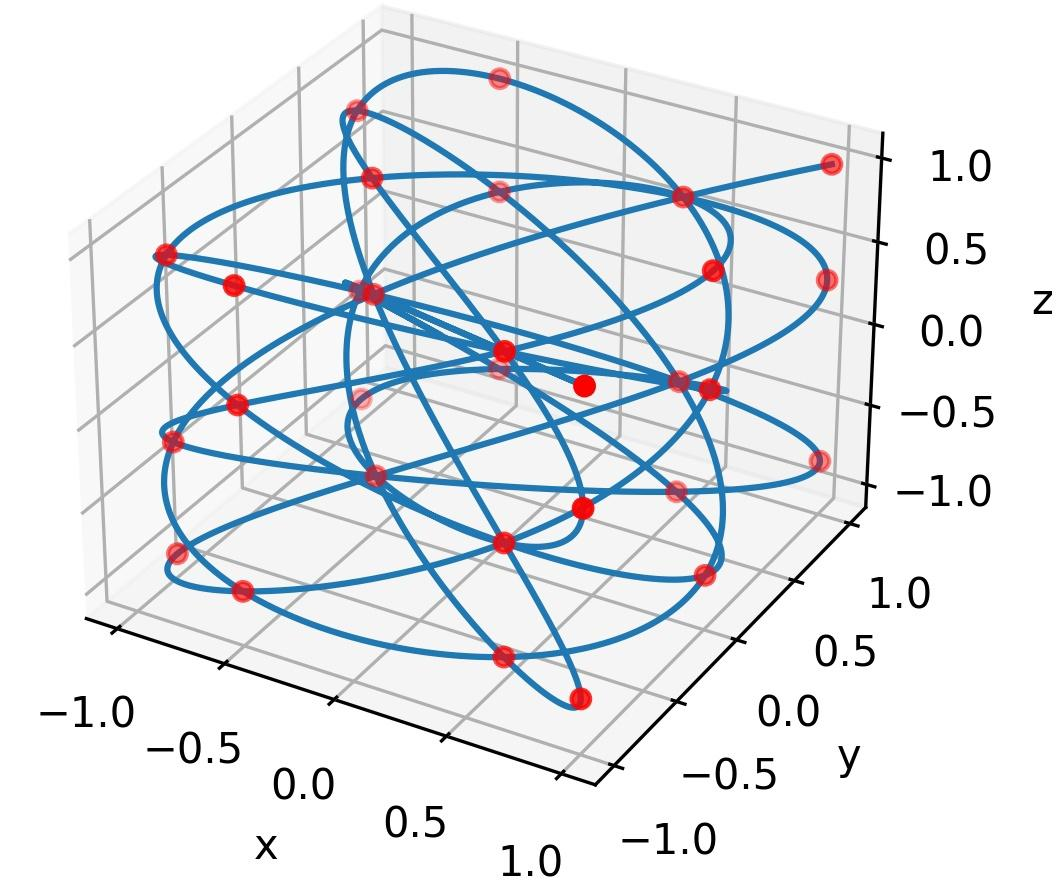
\includegraphics[width=0.5\linewidth]{../images/solution/chebLis.png}
    \captionof{figure}{Узлы Чебышева--Лиссажу в единичном кубе}
    \label{fig:chebLis}
\end{figure}

Теперь необходимо найти d-мерный полином, удовлетворяющий условию интерполяции.

Полиномы Чебышева имеют следующий вид:
\begin{equation*}
    T_{\gamma} (x) = \cos (\gamma \arccos (x)).
\end{equation*}

В узлах Чебышева--Лиссажу:
\begin{equation*}
    T_{\gamma} (z^n_i) = \cos \left(\gamma \arccos \left(\cos \left(\frac{i \pi}{n}\right) \right)\right)
     = \cos(\gamma \frac{i \pi}{n}) \equiv \chi_{\gamma}^n (i).
\end{equation*}

Определим d-мерные полиномы Чебышева как:
\begin{equation*}
    T_{\mathbf{\gamma}} = T_{\gamma_1} \cdot \dots \cdot T_{\gamma_d},
\end{equation*}
где $\mathbf{\gamma} \in \mathbb{N}^d_0$.
Они составляют ортогональный базис в d-мерном пространстве полиномов. Аналогично,
\begin{equation*}
    \chi_{\mathbf{\gamma}}^{\mathbf{n}} (\mathbf{i}) = \prod_{j=1}^{d} \cos(\gamma_j \frac{i_j \pi}{n_j}).
\end{equation*}
В свою очередь $\chi_{\mathbf{\gamma}}^{\mathbf{n}} (\mathbf{i})$ составляют базис в пространстве
функций $L^2$.

Этот факт дает возможность разложить, функцию $h$, заданную на узлах, по данному базису, чтобы
получить коэффициенты интерполяции:
\begin{equation*}
    \begin{cases*}
        h \approx \sum_{\mathbf{\gamma}} c_{\mathbf{\gamma}} (h) \chi_{\mathbf{\gamma}}^{\mathbf{n}}, \\
        c_{\mathbf{\gamma}} (h) = \frac{1}{|| \chi_{\mathbf{\gamma}}^{\mathbf{n}} ||^2}
        \left(h, \chi_{\mathbf{\gamma}}^{\mathbf{n}}\right).
    \end{cases*}
\end{equation*}

Вид базисных функций позволяет последовательно
применить дискретное косинус преобразование к каждой размерности для эффективного подсчета
коэффициентов. 

В результате функция может быть аппроксимирована линейной комбинацией произведений
многочленов Чебышева:
\begin{equation*}
    h \approx \sum_{\mathbf{\gamma}} c_{\gamma} T_\gamma.
\end{equation*}

В частном случае интерполяции 4-мерной функции плотности атмосферы
результат представим в виде:
\begin{equation*}
    \ln(\rho) \approx \sum_{i,j,k,l}^{n_1, n_2, n_3, n_4} 
    c_{i,j,k,l} T_i(r) T_j(\phi) T_k (\lambda) T_l (t),
\end{equation*}
где $T_\alpha$ -- полином Чебышева степени $\alpha$.

Интерполяция логарифма объяснятся тем фактом, что зависимость убывания
атмосферной плотности с высотой примерно экспоненциальная.

Точность интерполяции определяется количеством ячеек, на которое было разбито пространство,
и максимальной степенью полиномов по размерности для каждой ячейки. При построении
интерполянта расчет ячеек независим, что дает возможность вычислять коэффициенты в ячейках
параллельно на нескольких потоках.

Скорость интерполяции зависит от конфигурации интерполянта. Чем больше степени полиномов в
каждой ячейке, тем сильнее увеличивается время подсчета.

\subsection{Тестирование интерполяции}

Проведено тестирование точности различных конфигураций интерполянтов для модели NRLMSISE-00.
Диапазон интерполяции по расстоянию был выбран от 350 до 800 километров, интервал по времени
составил одни сутки. В ходе тестов была использована космическая погода за 11 января 2014 года.
Этот год соответствует высокой солнечной активности, что позволяет протестировать качество
интерполяции в сложных условиях.

Сетка для проверки работы алгоритма состояла из более 1 миллиона точек, равномерно
распределенных по области интерполяции. Для каждого интерполянта измерялась максимальная
ошибка на тестовой сетке, размер и величина ускорения по сравнению с прямым расчетом плотности.

Полный перебор по возможным конфигурациям и количеству ячеек интерполянтов сложен
из-за большого количества вариантов, времени, затрачиваемого на построение каждого интерполянта, и
занимаемой памяти. Поэтому поиск подходящих параметров проводился поэтапно.

Учитывая близкую к линейной зависимость логарифма плотности от высоты, для этой координаты
была выбрана наименьшая степень полинома -- 2. В рассмотрении остались наборы 
(2, 3, 5, 7), (2, 3, 7, 5), (2, 5, 3, 7), (2, 5, 7, 3), (2, 7, 3, 5),
(2, 7, 5, 3). Интерполянты для полиномов более
высоких порядков не строились из-за снижения производительности таких конфигураций и
существенного повышения затрат памяти для хранения коэффициентов.

Для каждого набора было зафиксировано количество ячеек по высоте -- 65. Количество ячеек
по широте, долготе и времени варьировалось от 5 до 50. Эмпирически определялось
количество ячеек для достижения точности при заданном разбиении по высоте. Далее
для интерполянта с максимальным числом ячеек по широте, долготе и времени варьировалось
количество ячеек по высоте и определялась точность, достижимая с такими параметрами.

На рис. \ref{fig:atmo:2357} -- \ref{fig:atmo:2753} представлены зависимости относительной ошибки от количества ячеек по
конкретной координате интерполянта. Для времени фиксировалось
максимальное количество ячеек по остальным координатам. Для долготы и широты
фиксировалось наиболее плотное разбиение по широте и долготе соответственно, а диапазон
соответствует вариации количества ячеек по времени.

\begin{figure}[h!]
    \centering
    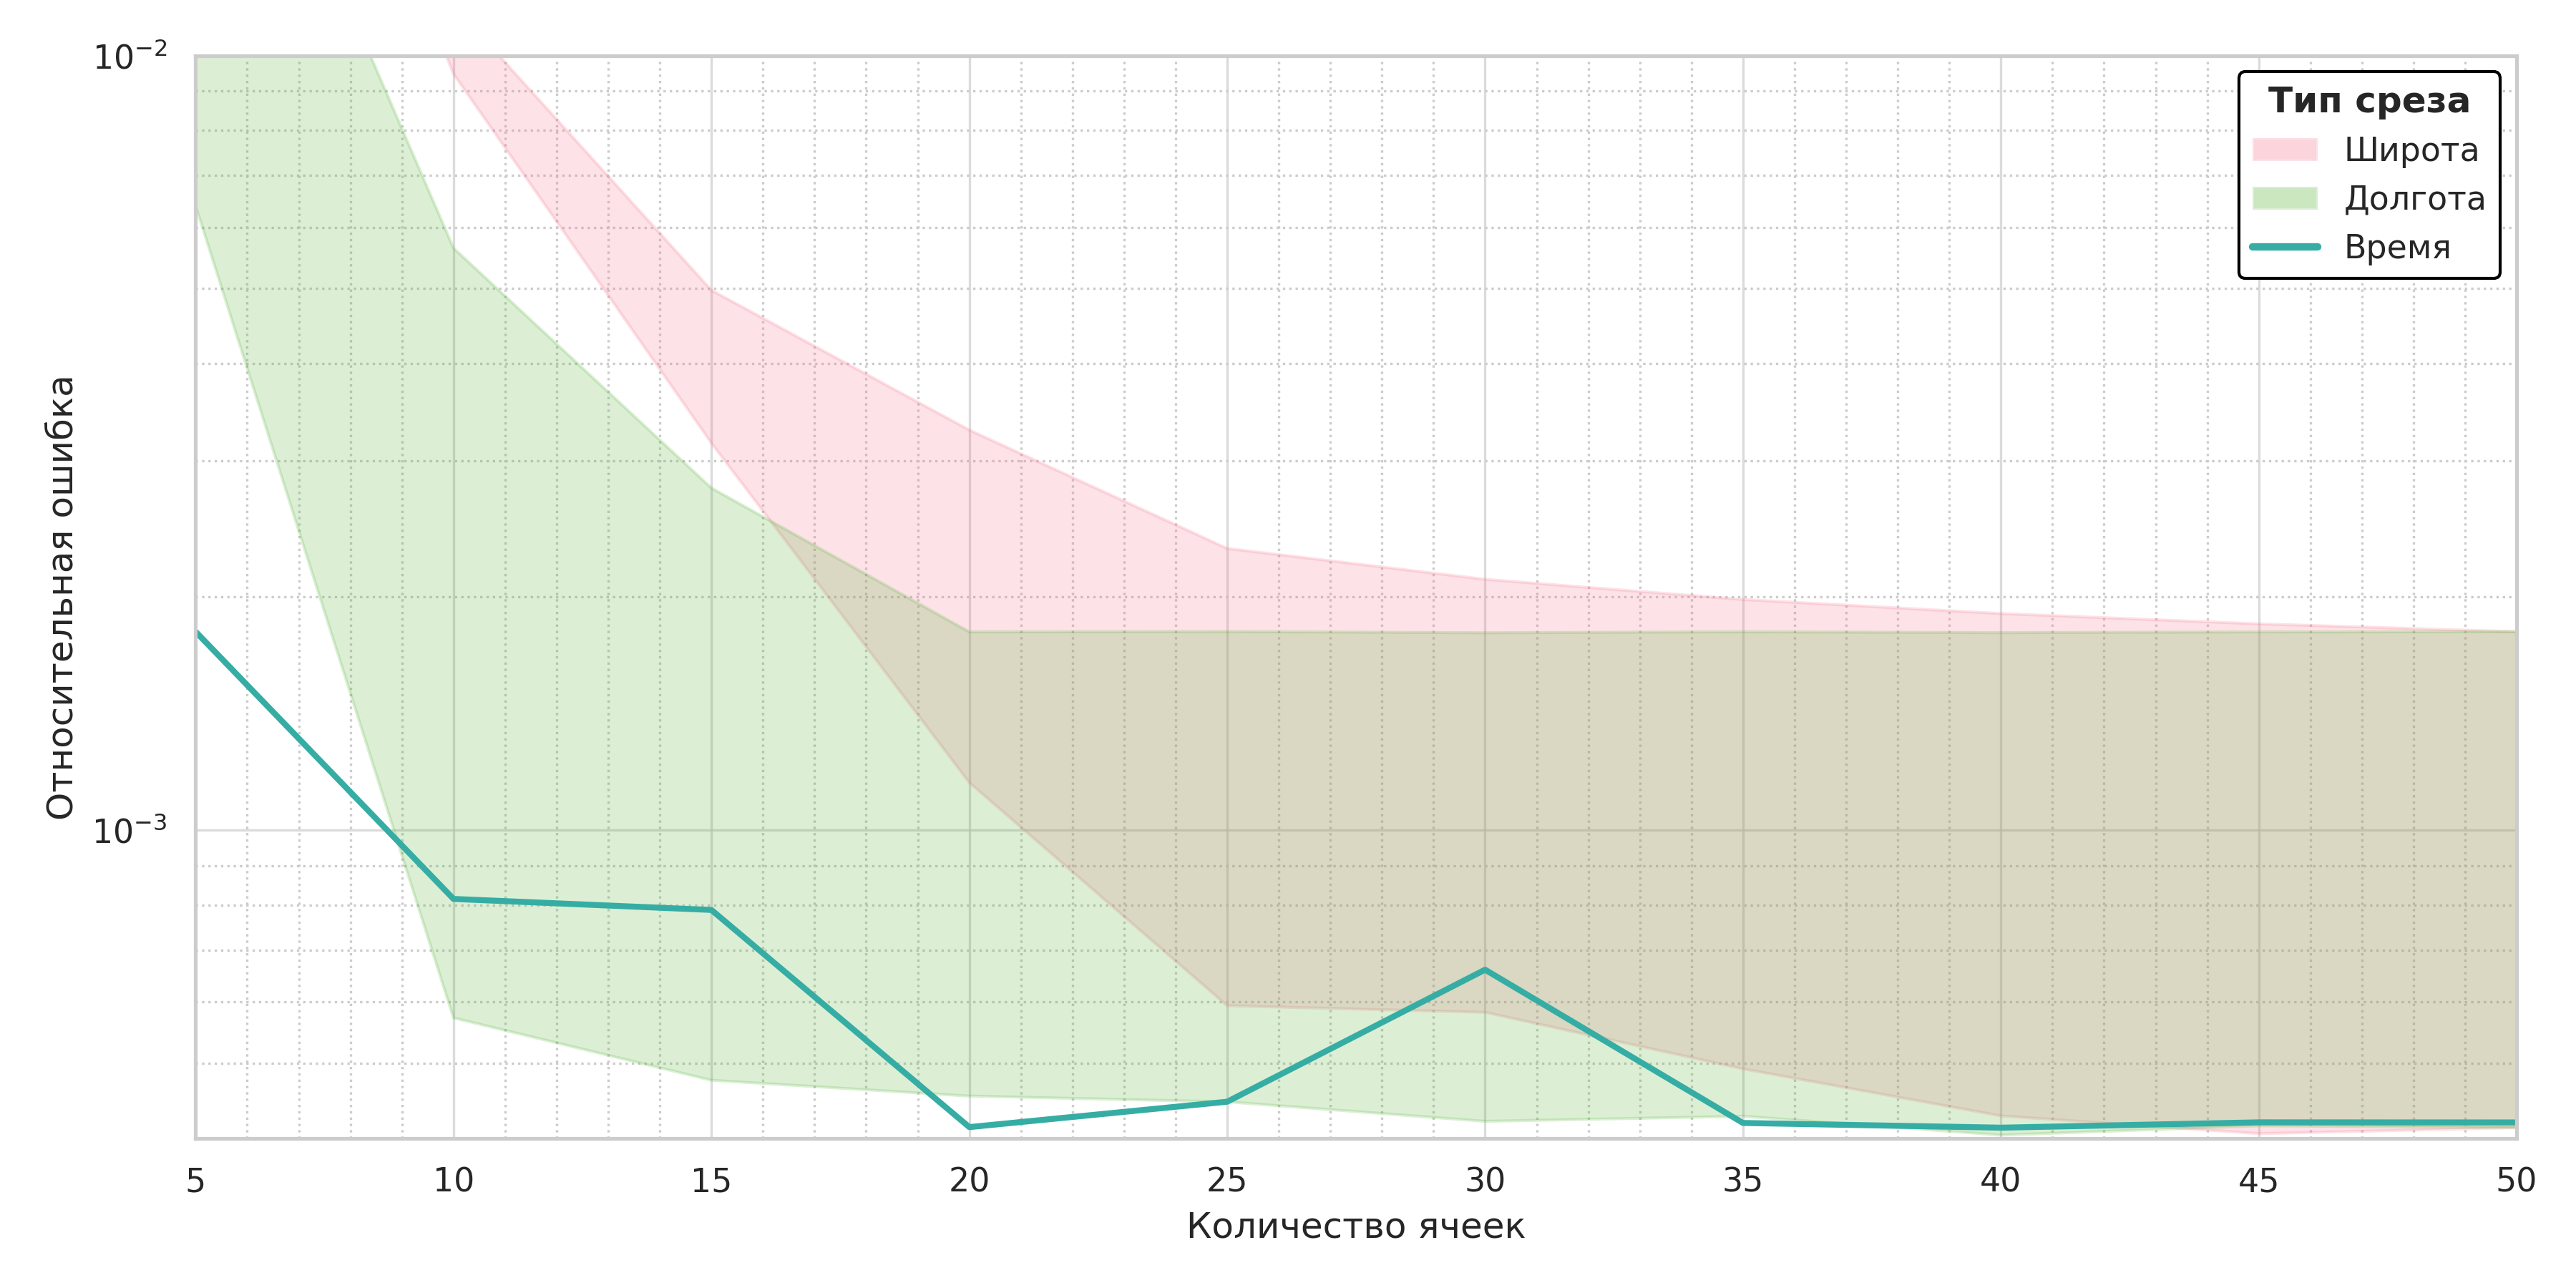
\includegraphics[width=\linewidth]{../images/solution/atmo/2357.png}
    \captionof{figure}{Зависимость ошибки от количества ячеек интерполянта для конфигурации (2, 3, 5, 7)}
    \label{fig:atmo:2357}
 \end{figure}

 \begin{figure}[h!]
    \centering
    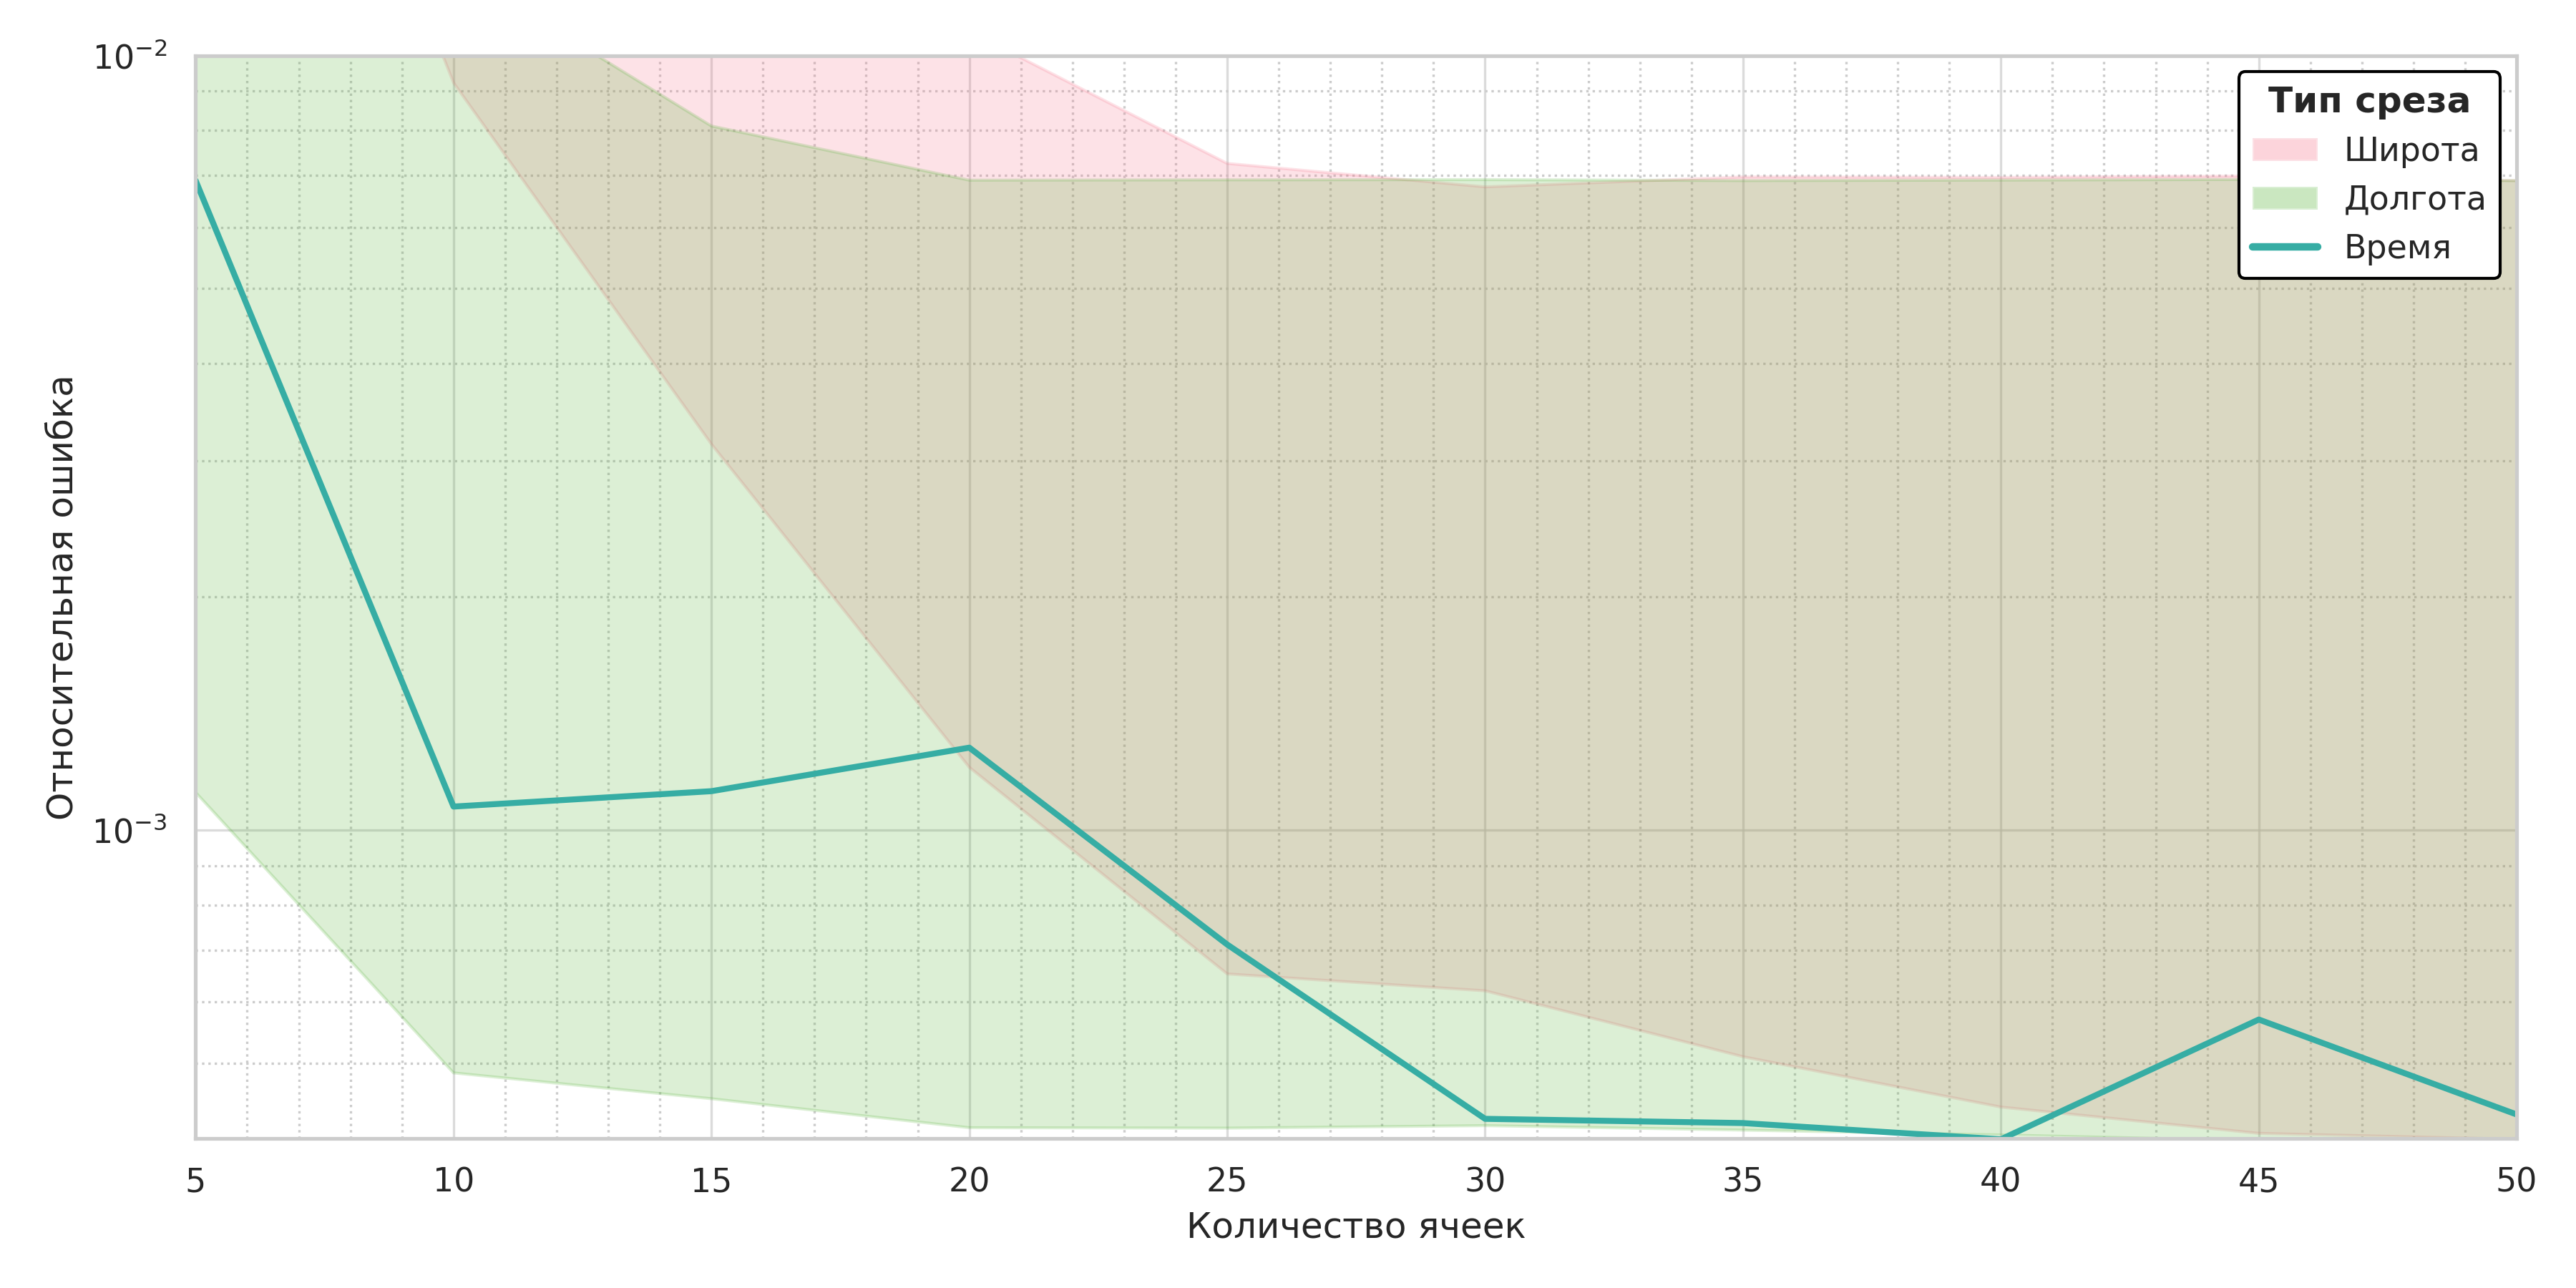
\includegraphics[width=\linewidth]{../images/solution/atmo/2375.png}
    \captionof{figure}{Зависимость ошибки от количества ячеек интерполянта для конфигурации (2, 3, 7, 5)}
    \label{fig:atmo:2375}
 \end{figure}

 \begin{figure}[h!]
    \centering
    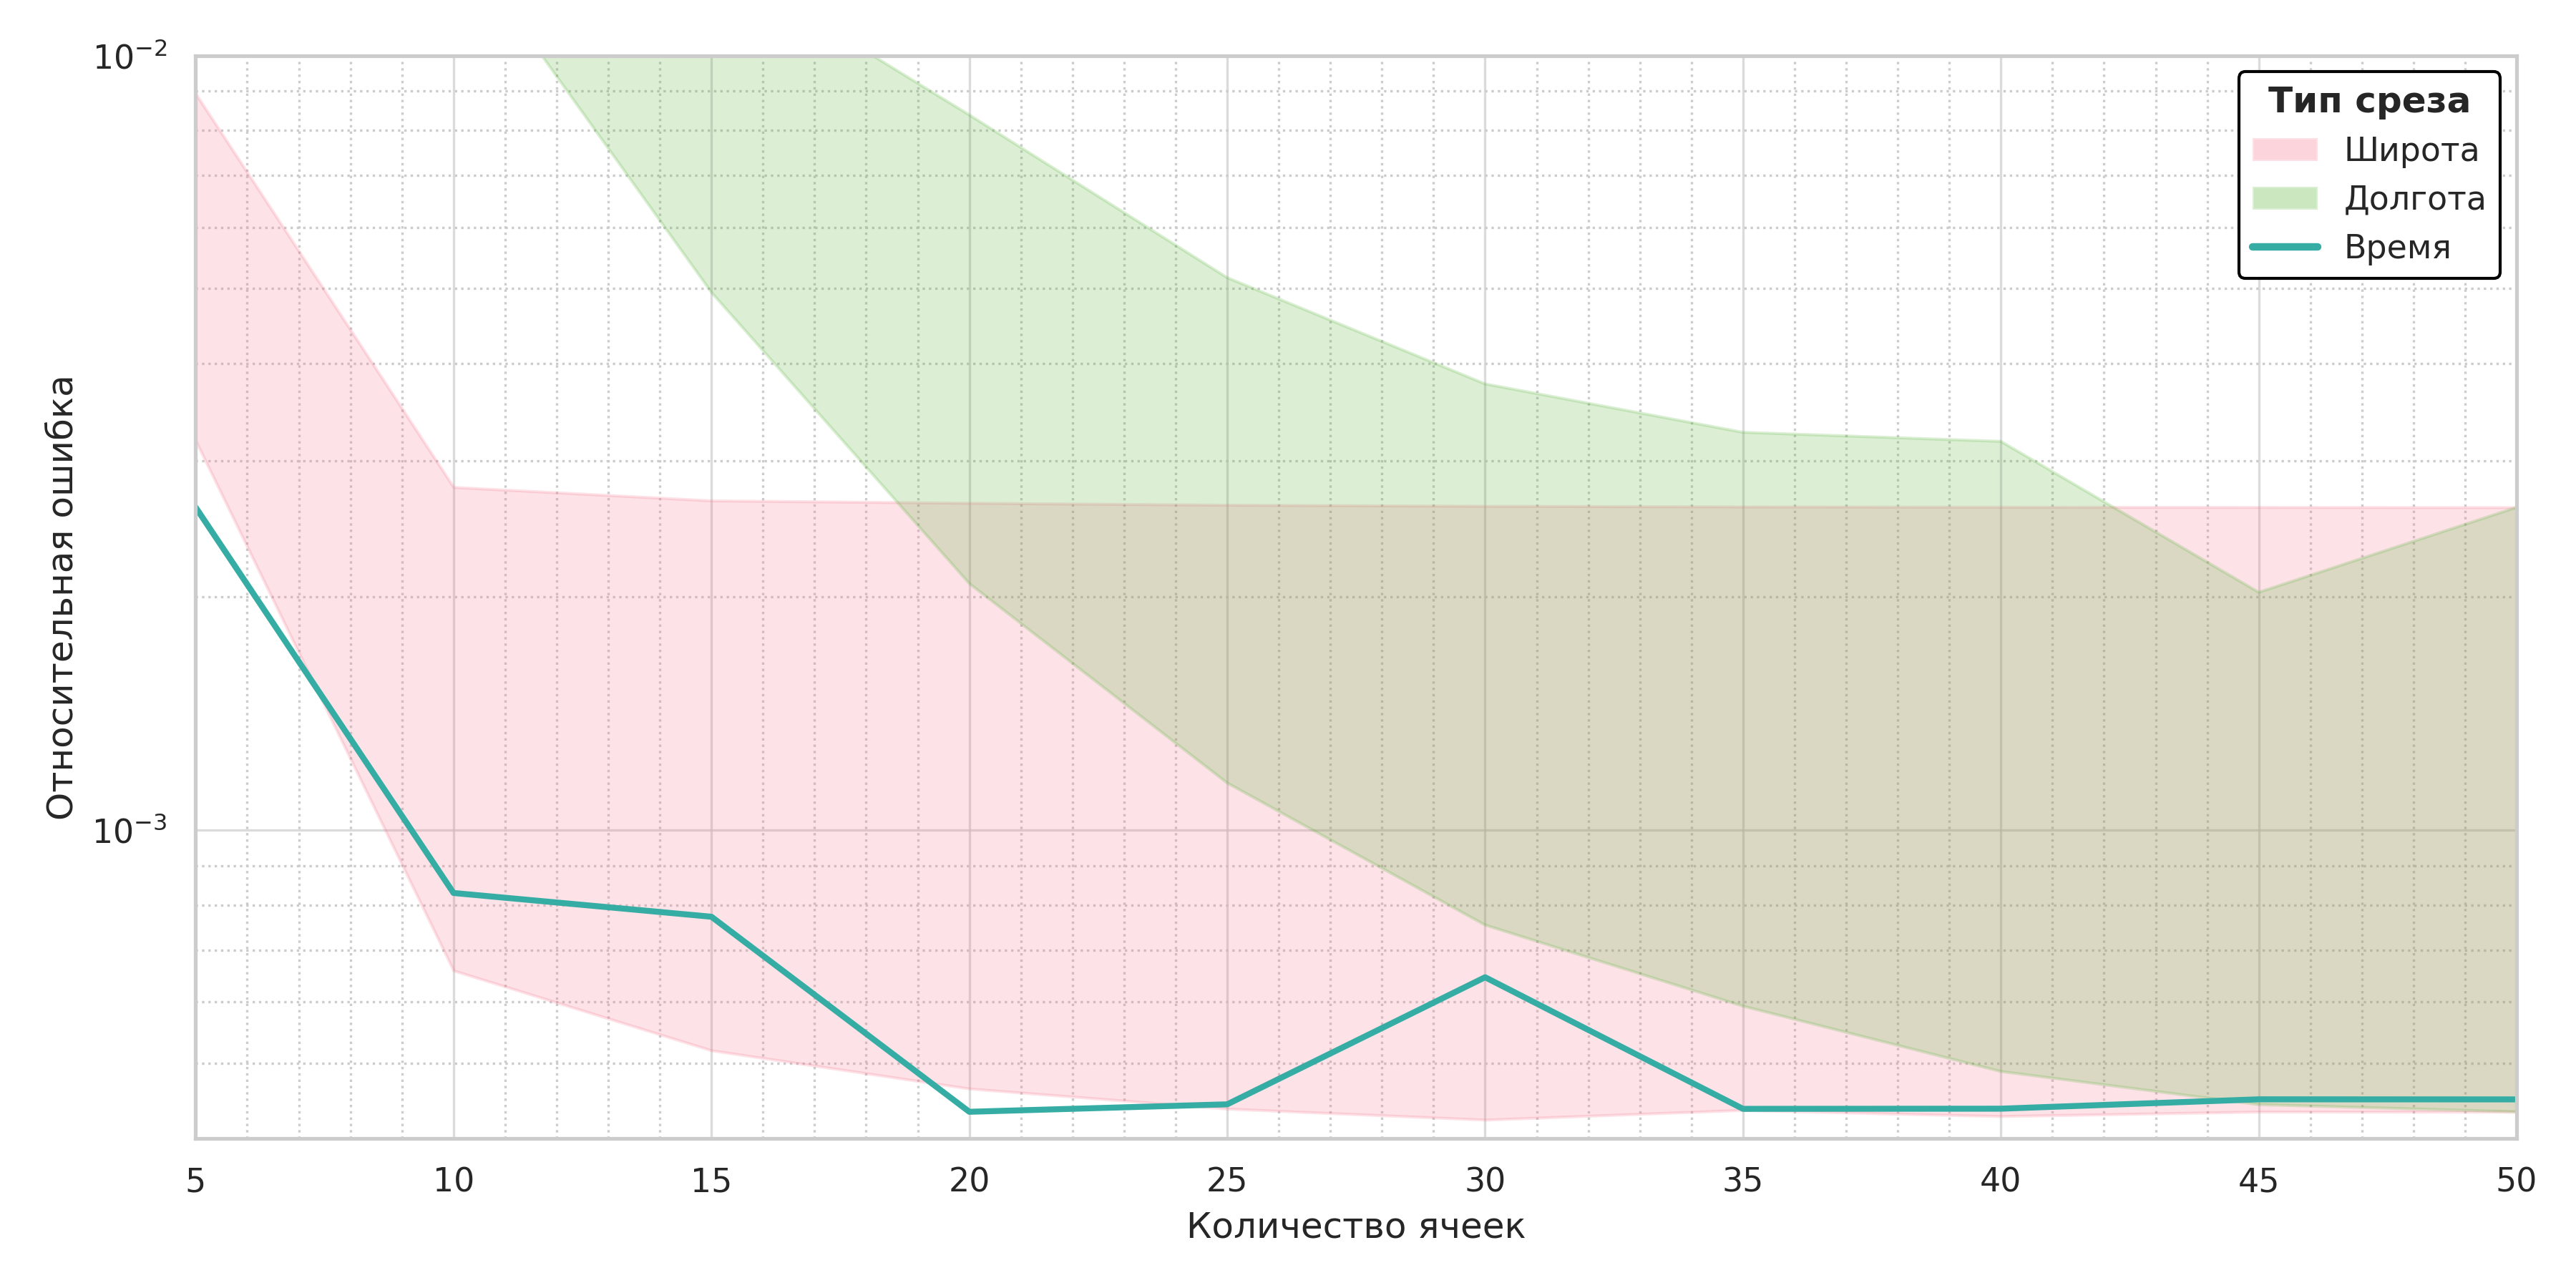
\includegraphics[width=\linewidth]{../images/solution/atmo/2537.png}
    \captionof{figure}{Зависимость ошибки от количества ячеек интерполянта для конфигурации (2, 5, 3, 7)}
    \label{fig:atmo:2537}
 \end{figure}

 \begin{figure}[h!]
    \centering
    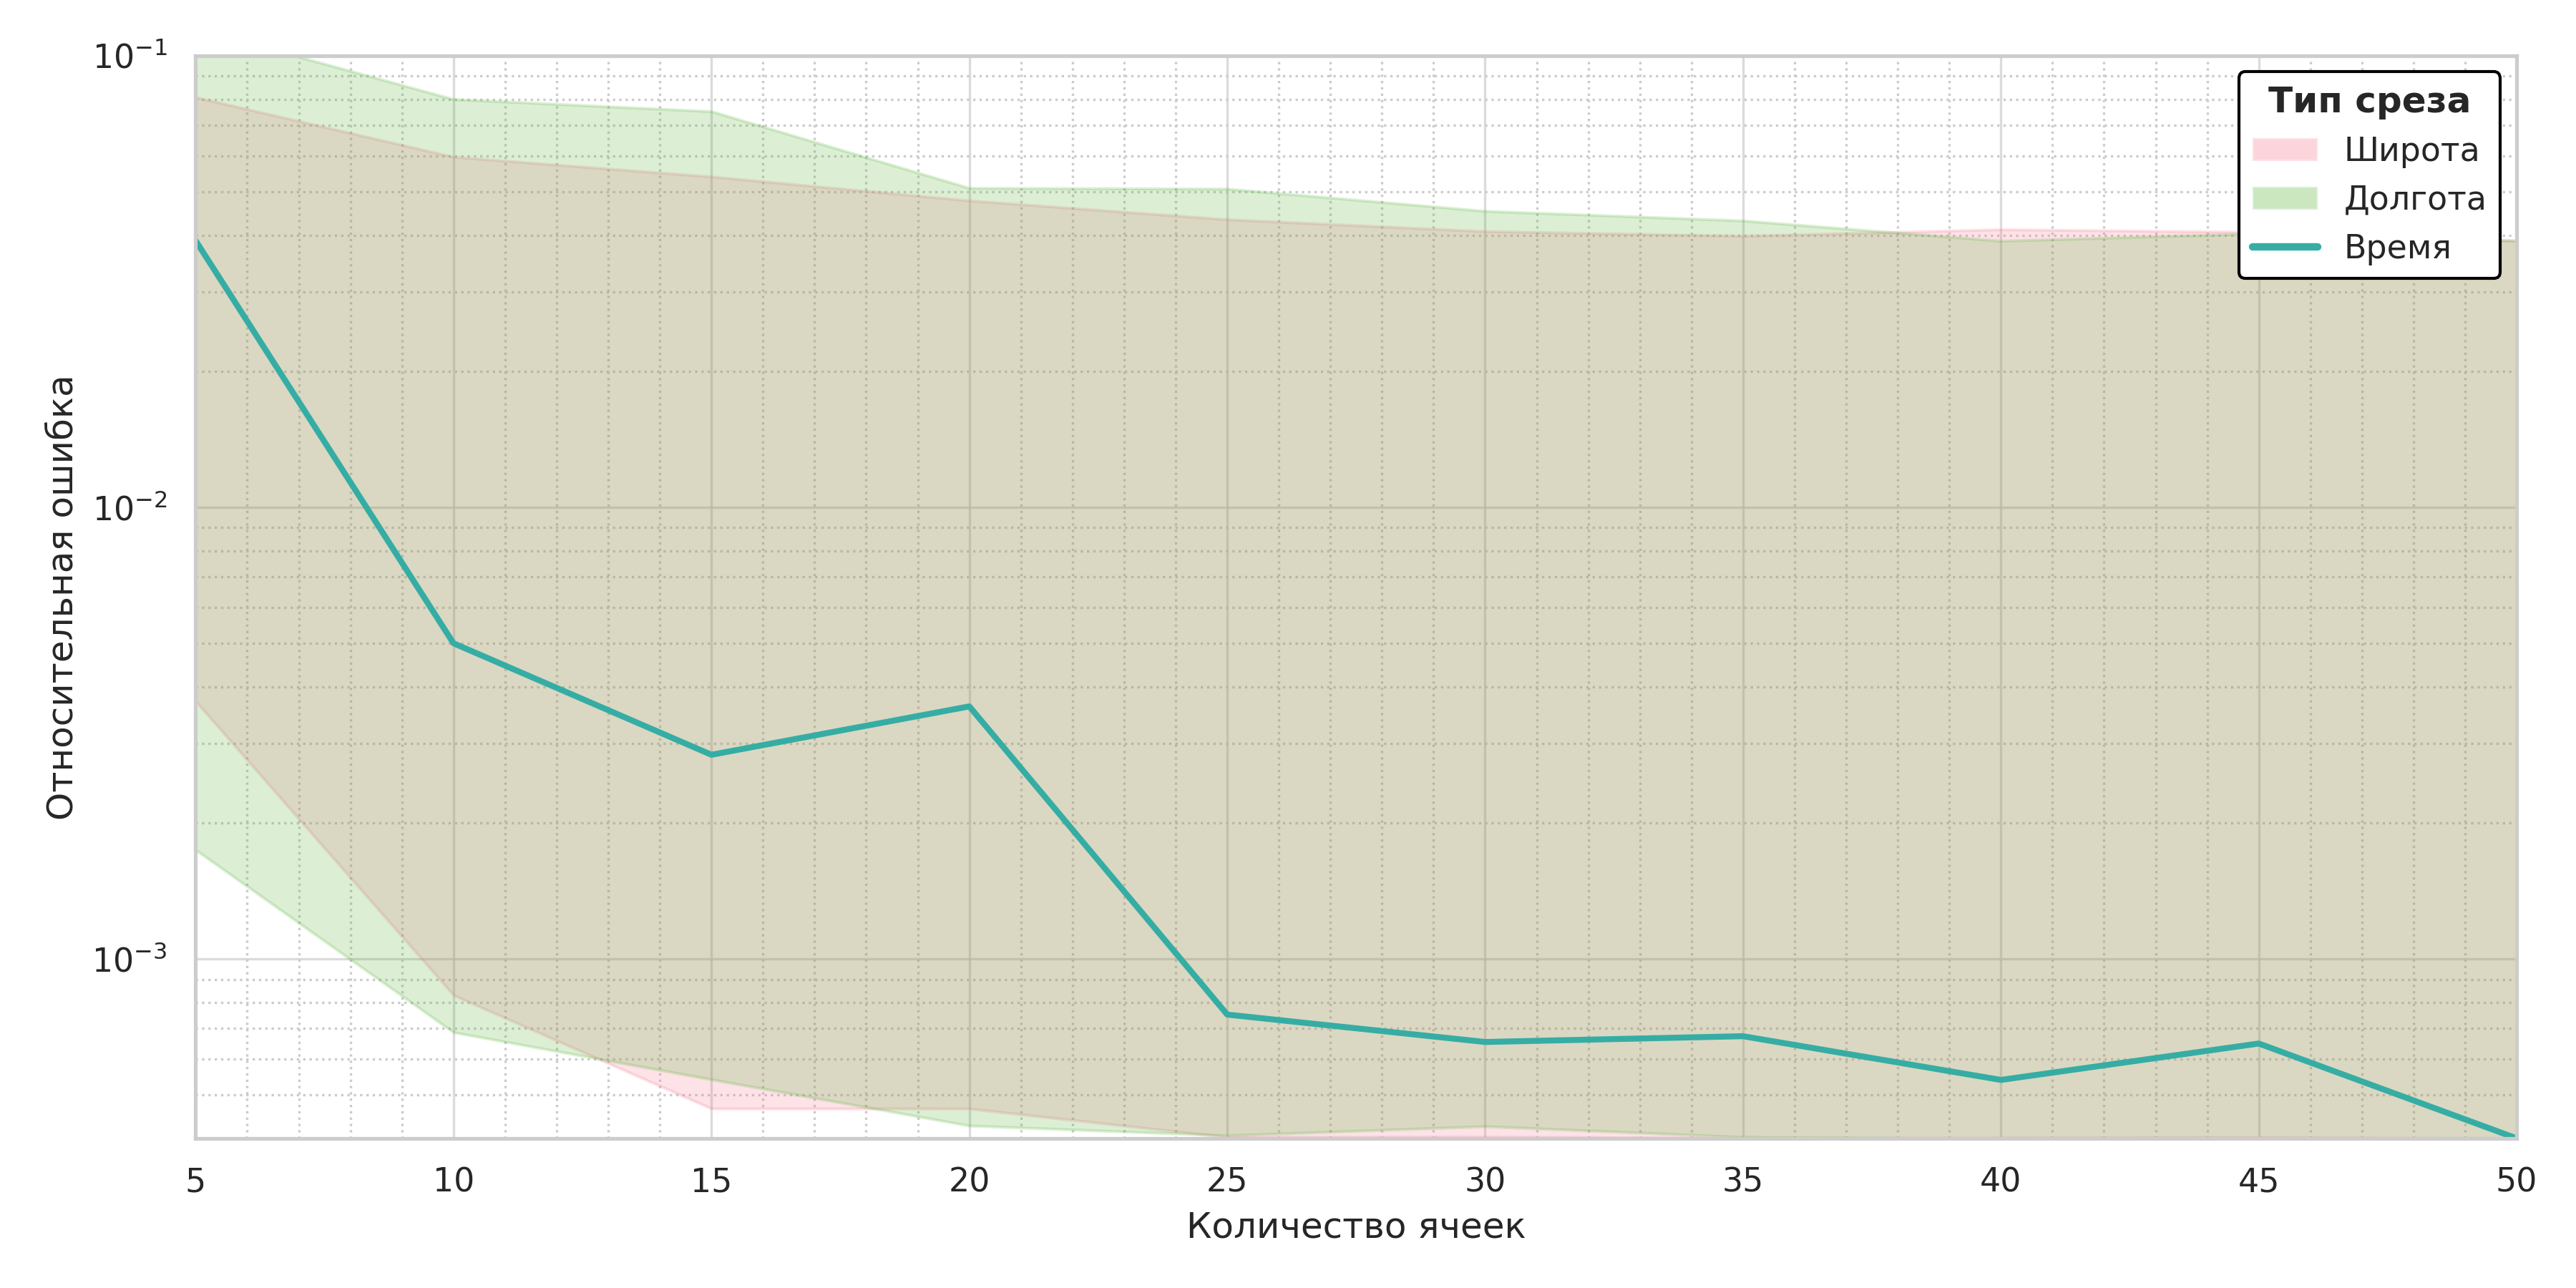
\includegraphics[width=\linewidth]{../images/solution/atmo/2573.png}
    \captionof{figure}{Зависимость ошибки от количества ячеек интерполянта для конфигурации (2, 5, 7, 3)}
    \label{fig:atmo:2573}
 \end{figure}

 \begin{figure}[h!]
    \centering
    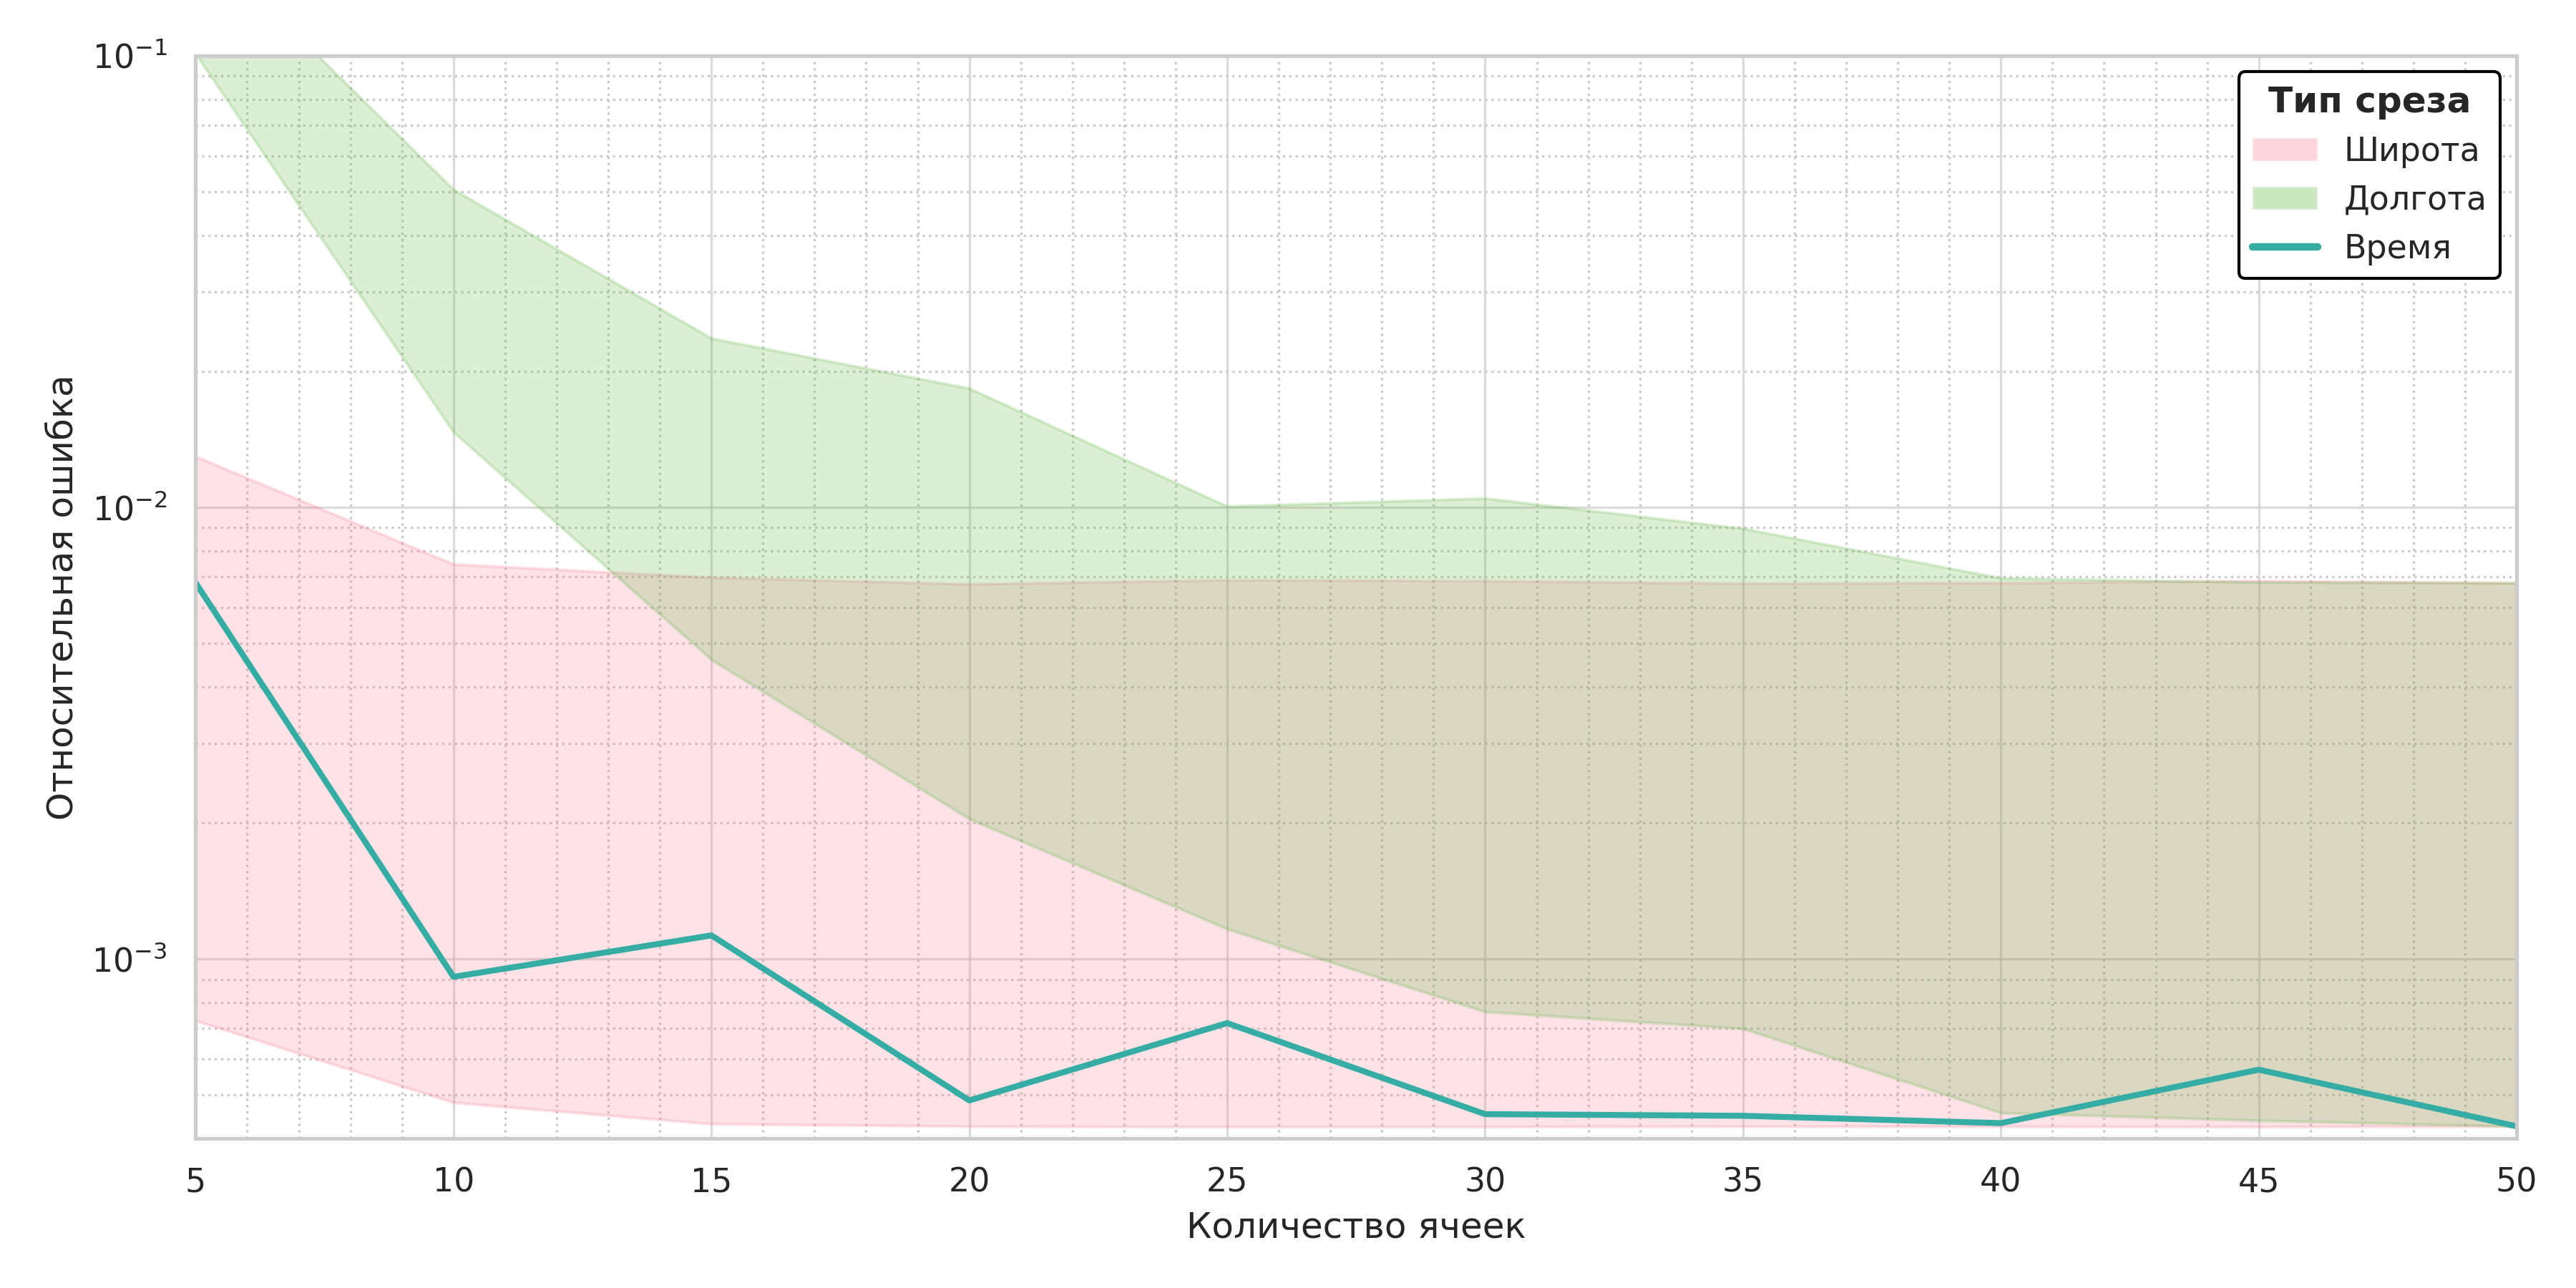
\includegraphics[width=\linewidth]{../images/solution/atmo/2735.png}
    \captionof{figure}{Зависимость ошибки от количества ячеек интерполянта для конфигурации (2, 7, 3, 5)}
    \label{fig:atmo:2735}
 \end{figure}

 \begin{figure}[h!]
    \centering
    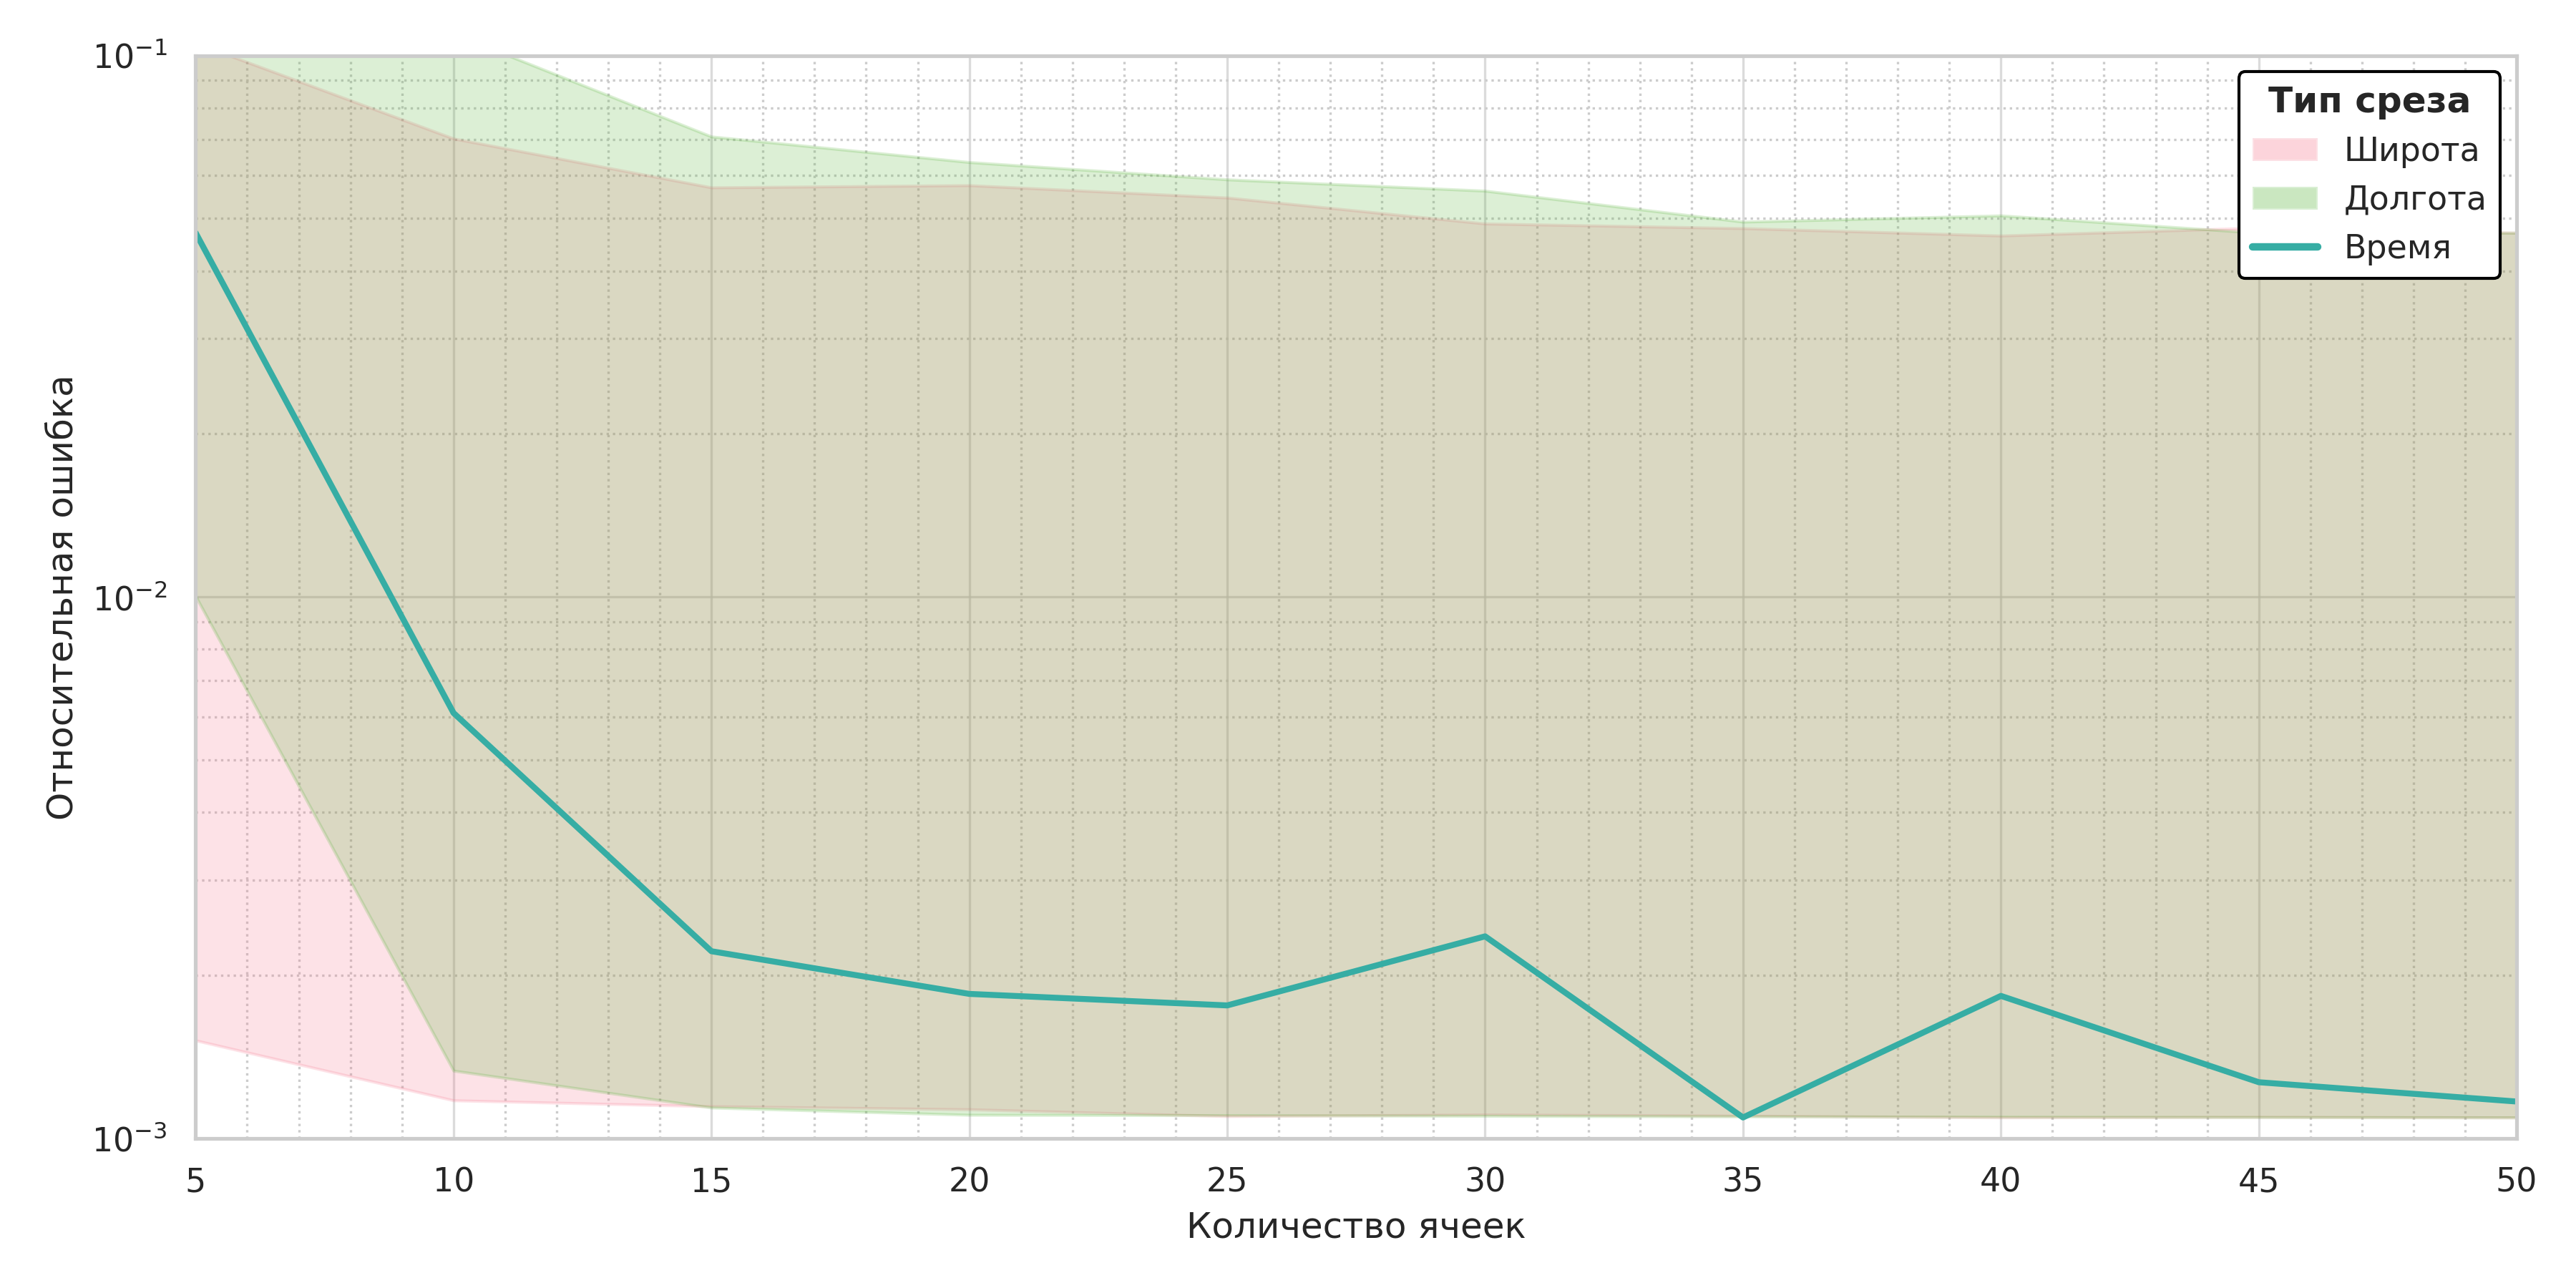
\includegraphics[width=\linewidth]{../images/solution/atmo/2753.png}
    \captionof{figure}{Зависимость ошибки от количества ячеек интерполянта для конфигурации (2, 7, 5, 3)}
    \label{fig:atmo:2753}
 \end{figure}

 Из графиков видно, что максимальная точность интерполянтов в тестах составила $4 \cdot 10^{-4}$.
 По срезам можно определить количество ячеек по каждой координате, которого достаточно для достижения
 предельной точности. Чем больше степень во времени, тем уже диапазон по широте и долготе. Это объясняется тем,
 что для достижения максимальной точности при заданном количестве ячеек по расстоянию
 требуется меньше ячеек по времени. На рис. \ref{fig:atmo:2357_heatmap} -- \ref{fig:atmo:2753_heatmap} изображены карты
 ошибок для разных конфигураций. Градиент на них направлен вдоль оси, соответствующей
 координате с наименьшей степенью в ячейке.

 Срез по количеству радиальных ячеек (рис. \ref{fig:atmo:2357_rho}) отражает тенденцию быстрого спада ошибки в области
 10 -- 30 и замедления спада далее. В окретсности 65 угол наклона графика мал, следовательно,
 выбор начального приближения количества ячеек был верным.

 \begin{figure}[h!]
    \centering
    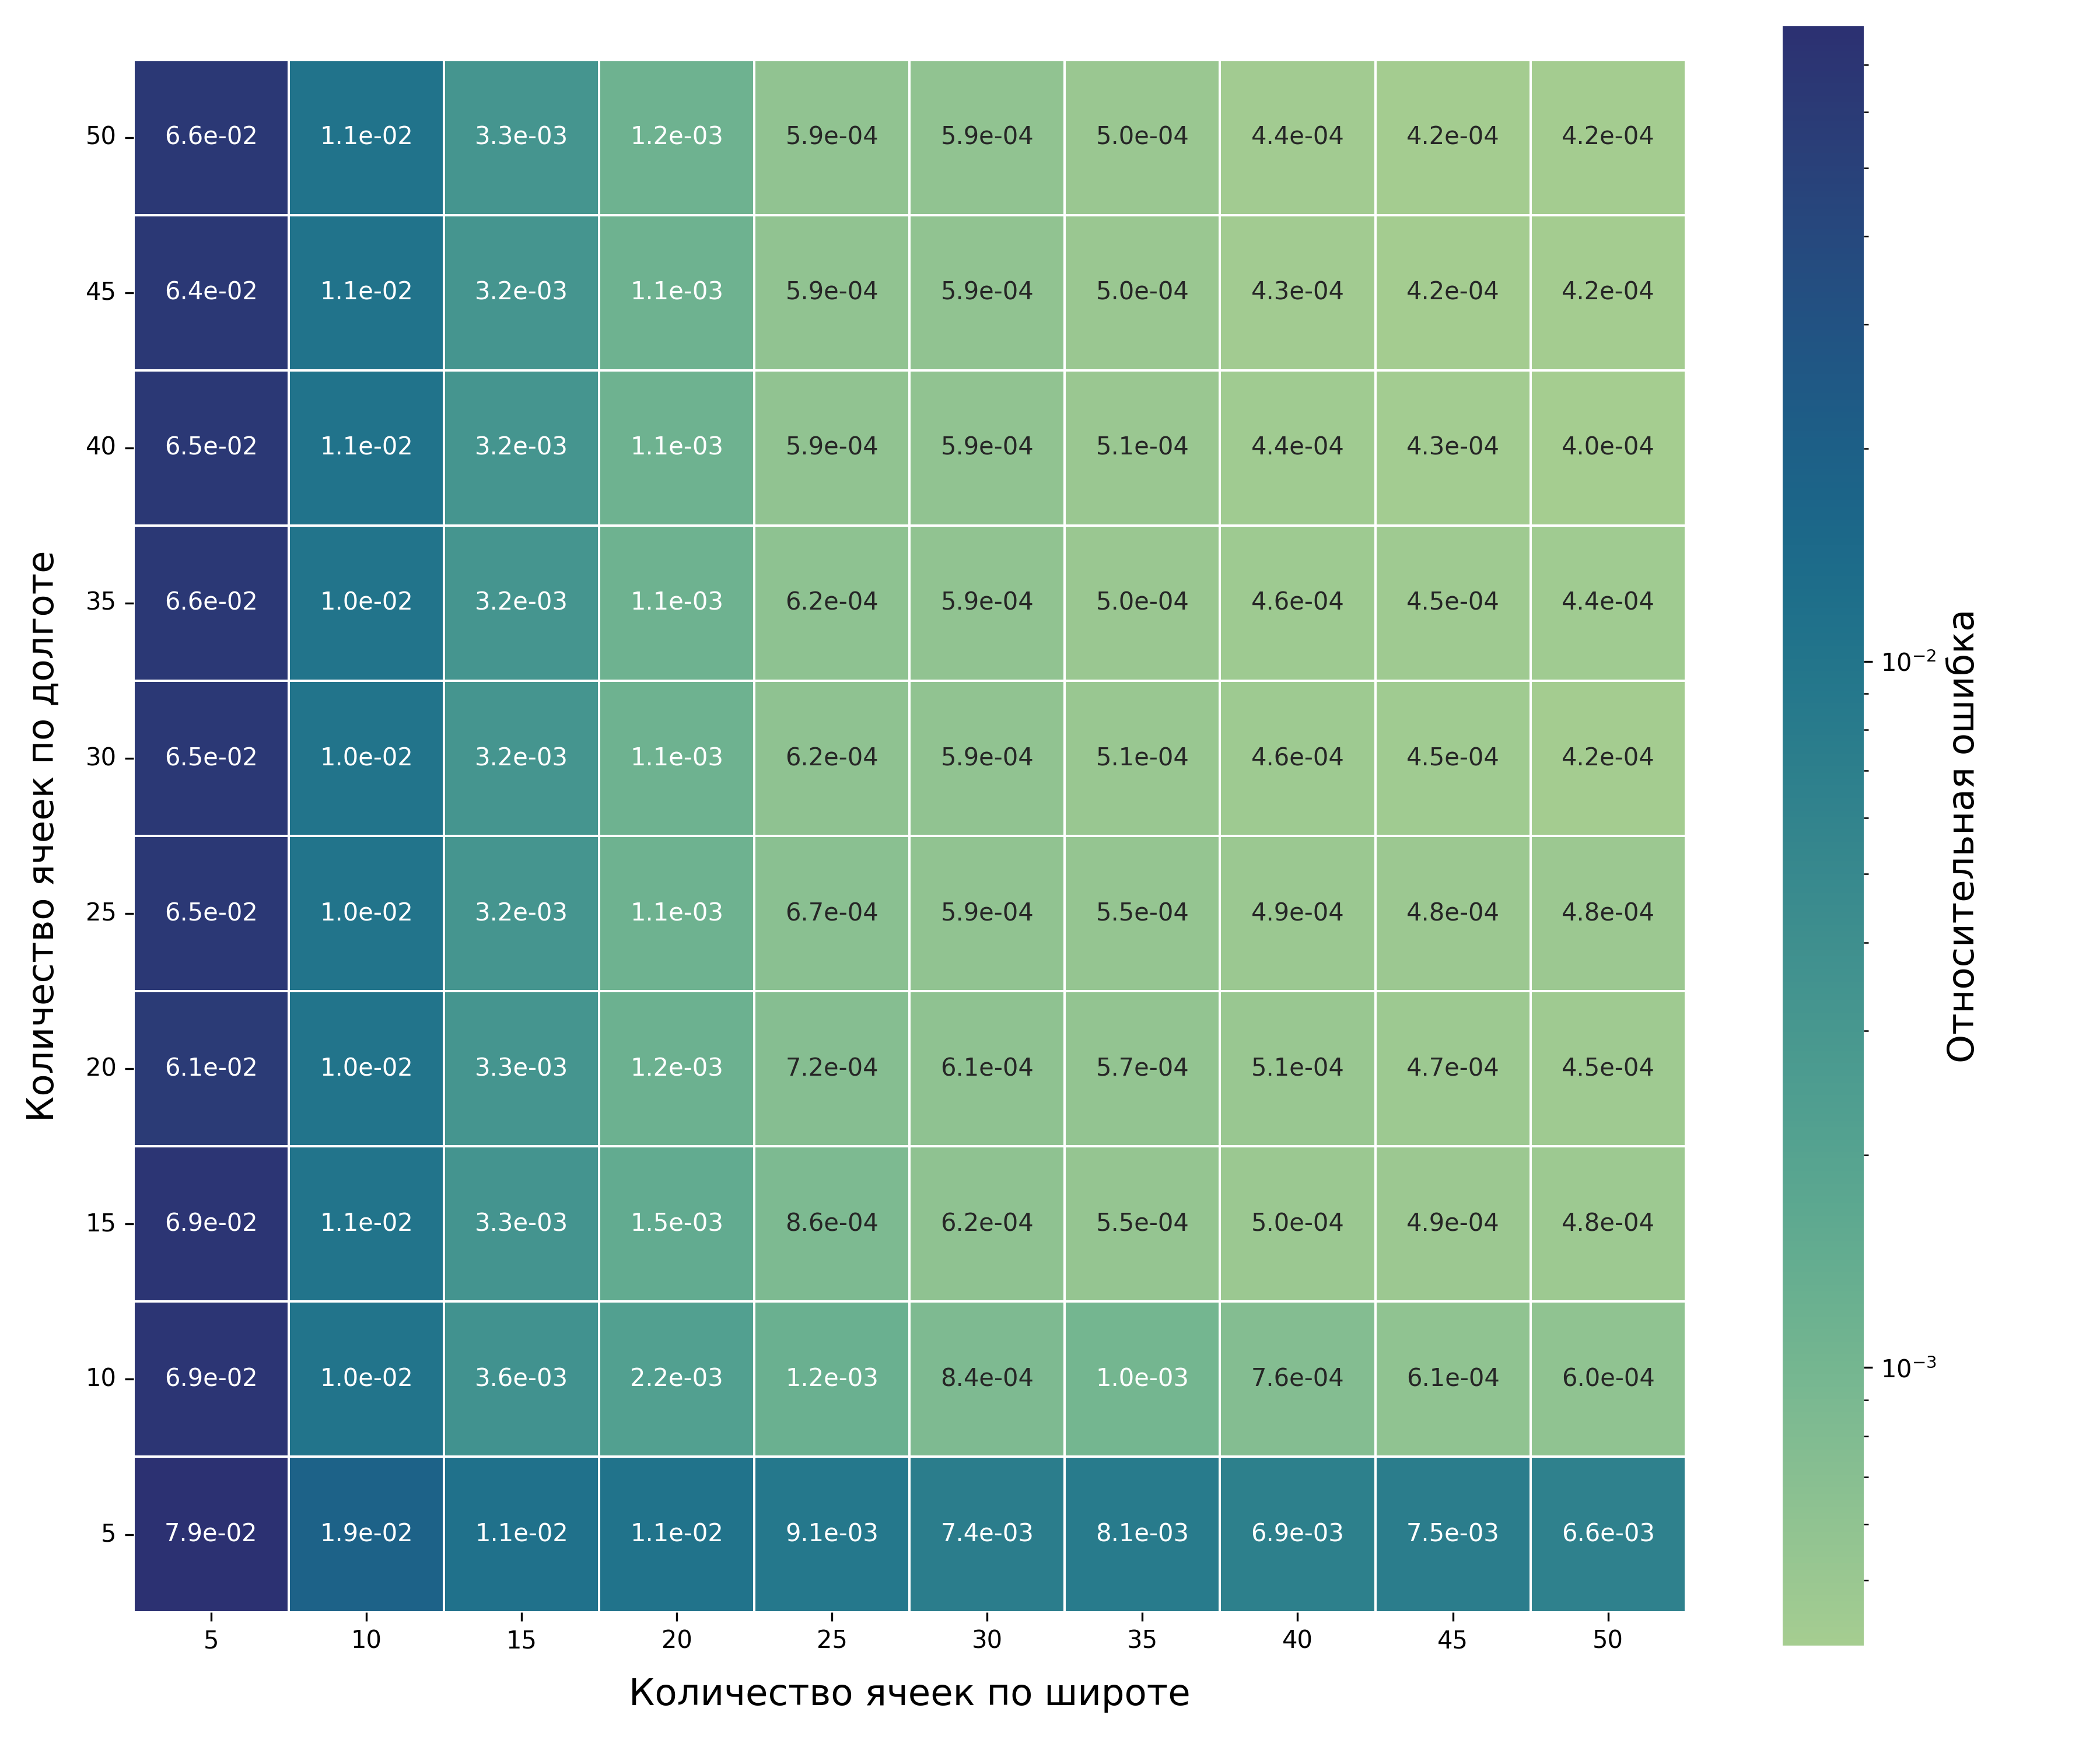
\includegraphics[width=0.85\linewidth]{../images/solution/atmo/2357_heatmap.png}
    \captionof{figure}{Карта ошибок для конфигурации (2, 3, 5, 7)}
    \label{fig:atmo:2357_heatmap}
 \end{figure}

 \begin{figure}[h!]
    \centering
    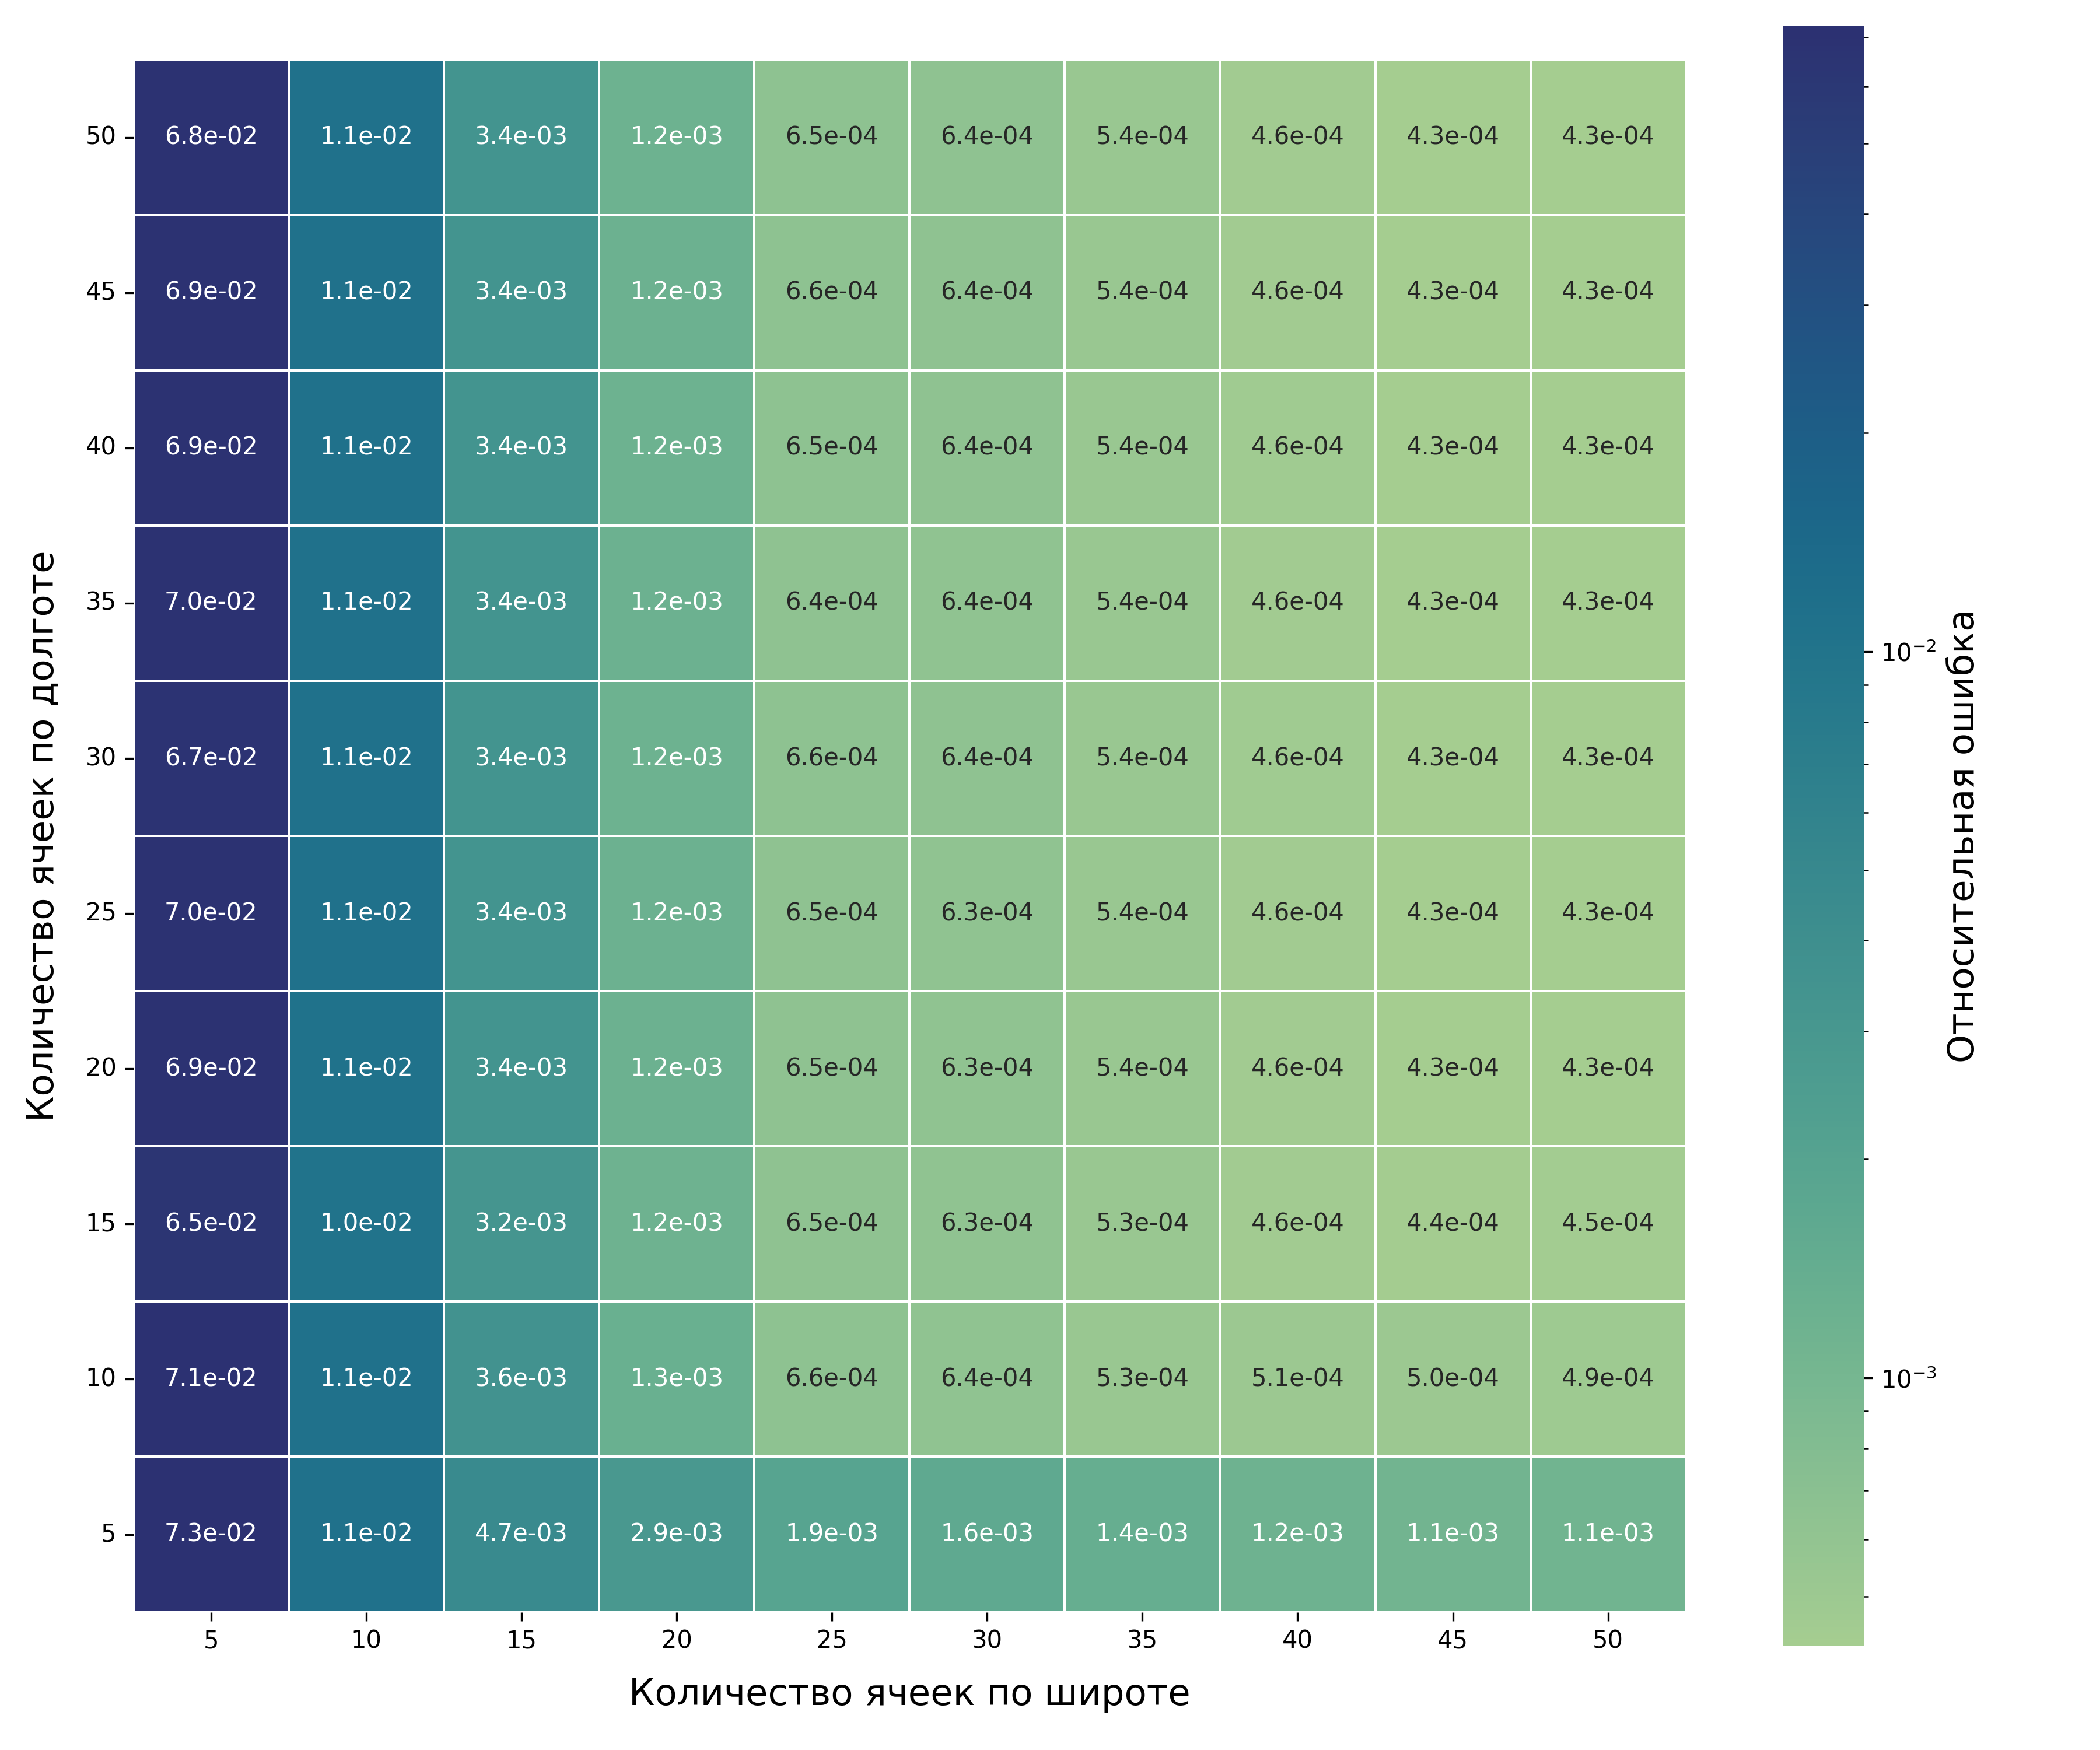
\includegraphics[width=0.85\linewidth]{../images/solution/atmo/2375_heatmap.png}
    \captionof{figure}{Карта ошибок для конфигурации (2, 3, 7, 5)}
    \label{fig:atmo:2375_heatmap}
 \end{figure}

 \begin{figure}[h!]
    \centering
    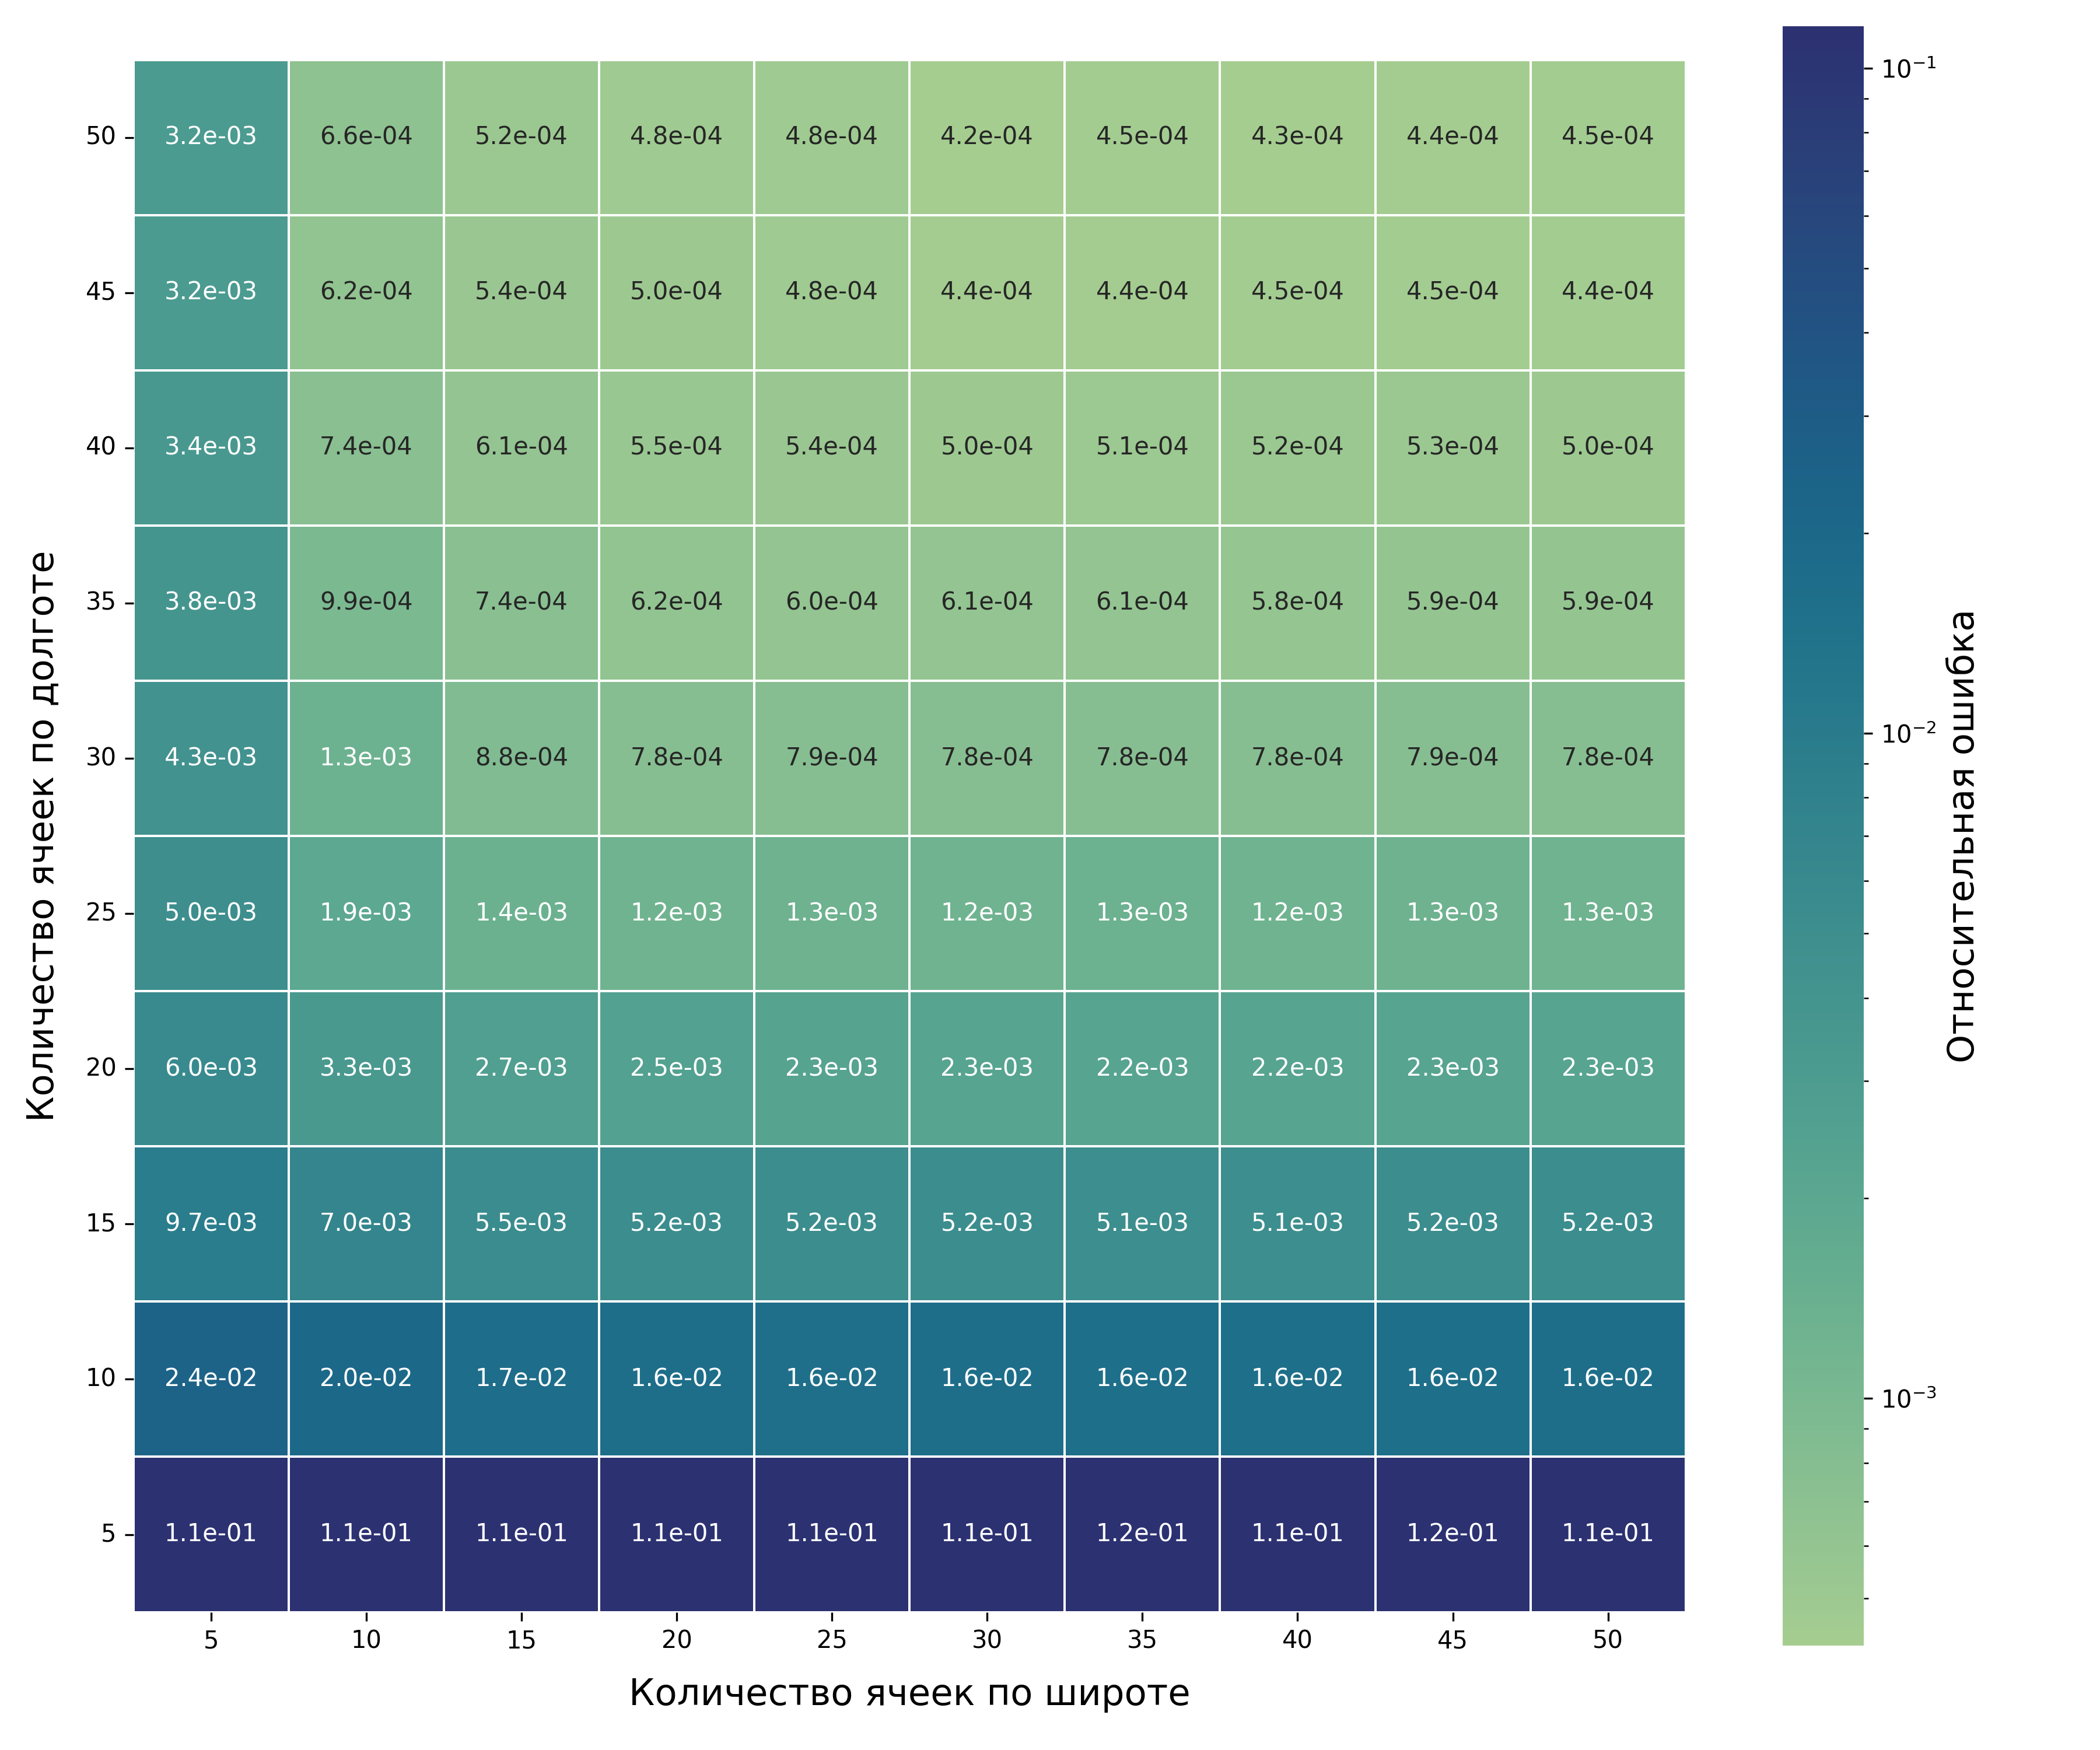
\includegraphics[width=0.85\linewidth]{../images/solution/atmo/2537_heatmap.png}
    \captionof{figure}{Карта ошибок для конфигурации (2, 5, 3, 7)}
    \label{fig:atmo:2537_heatmap}
 \end{figure}

 \begin{figure}[h!]
    \centering
    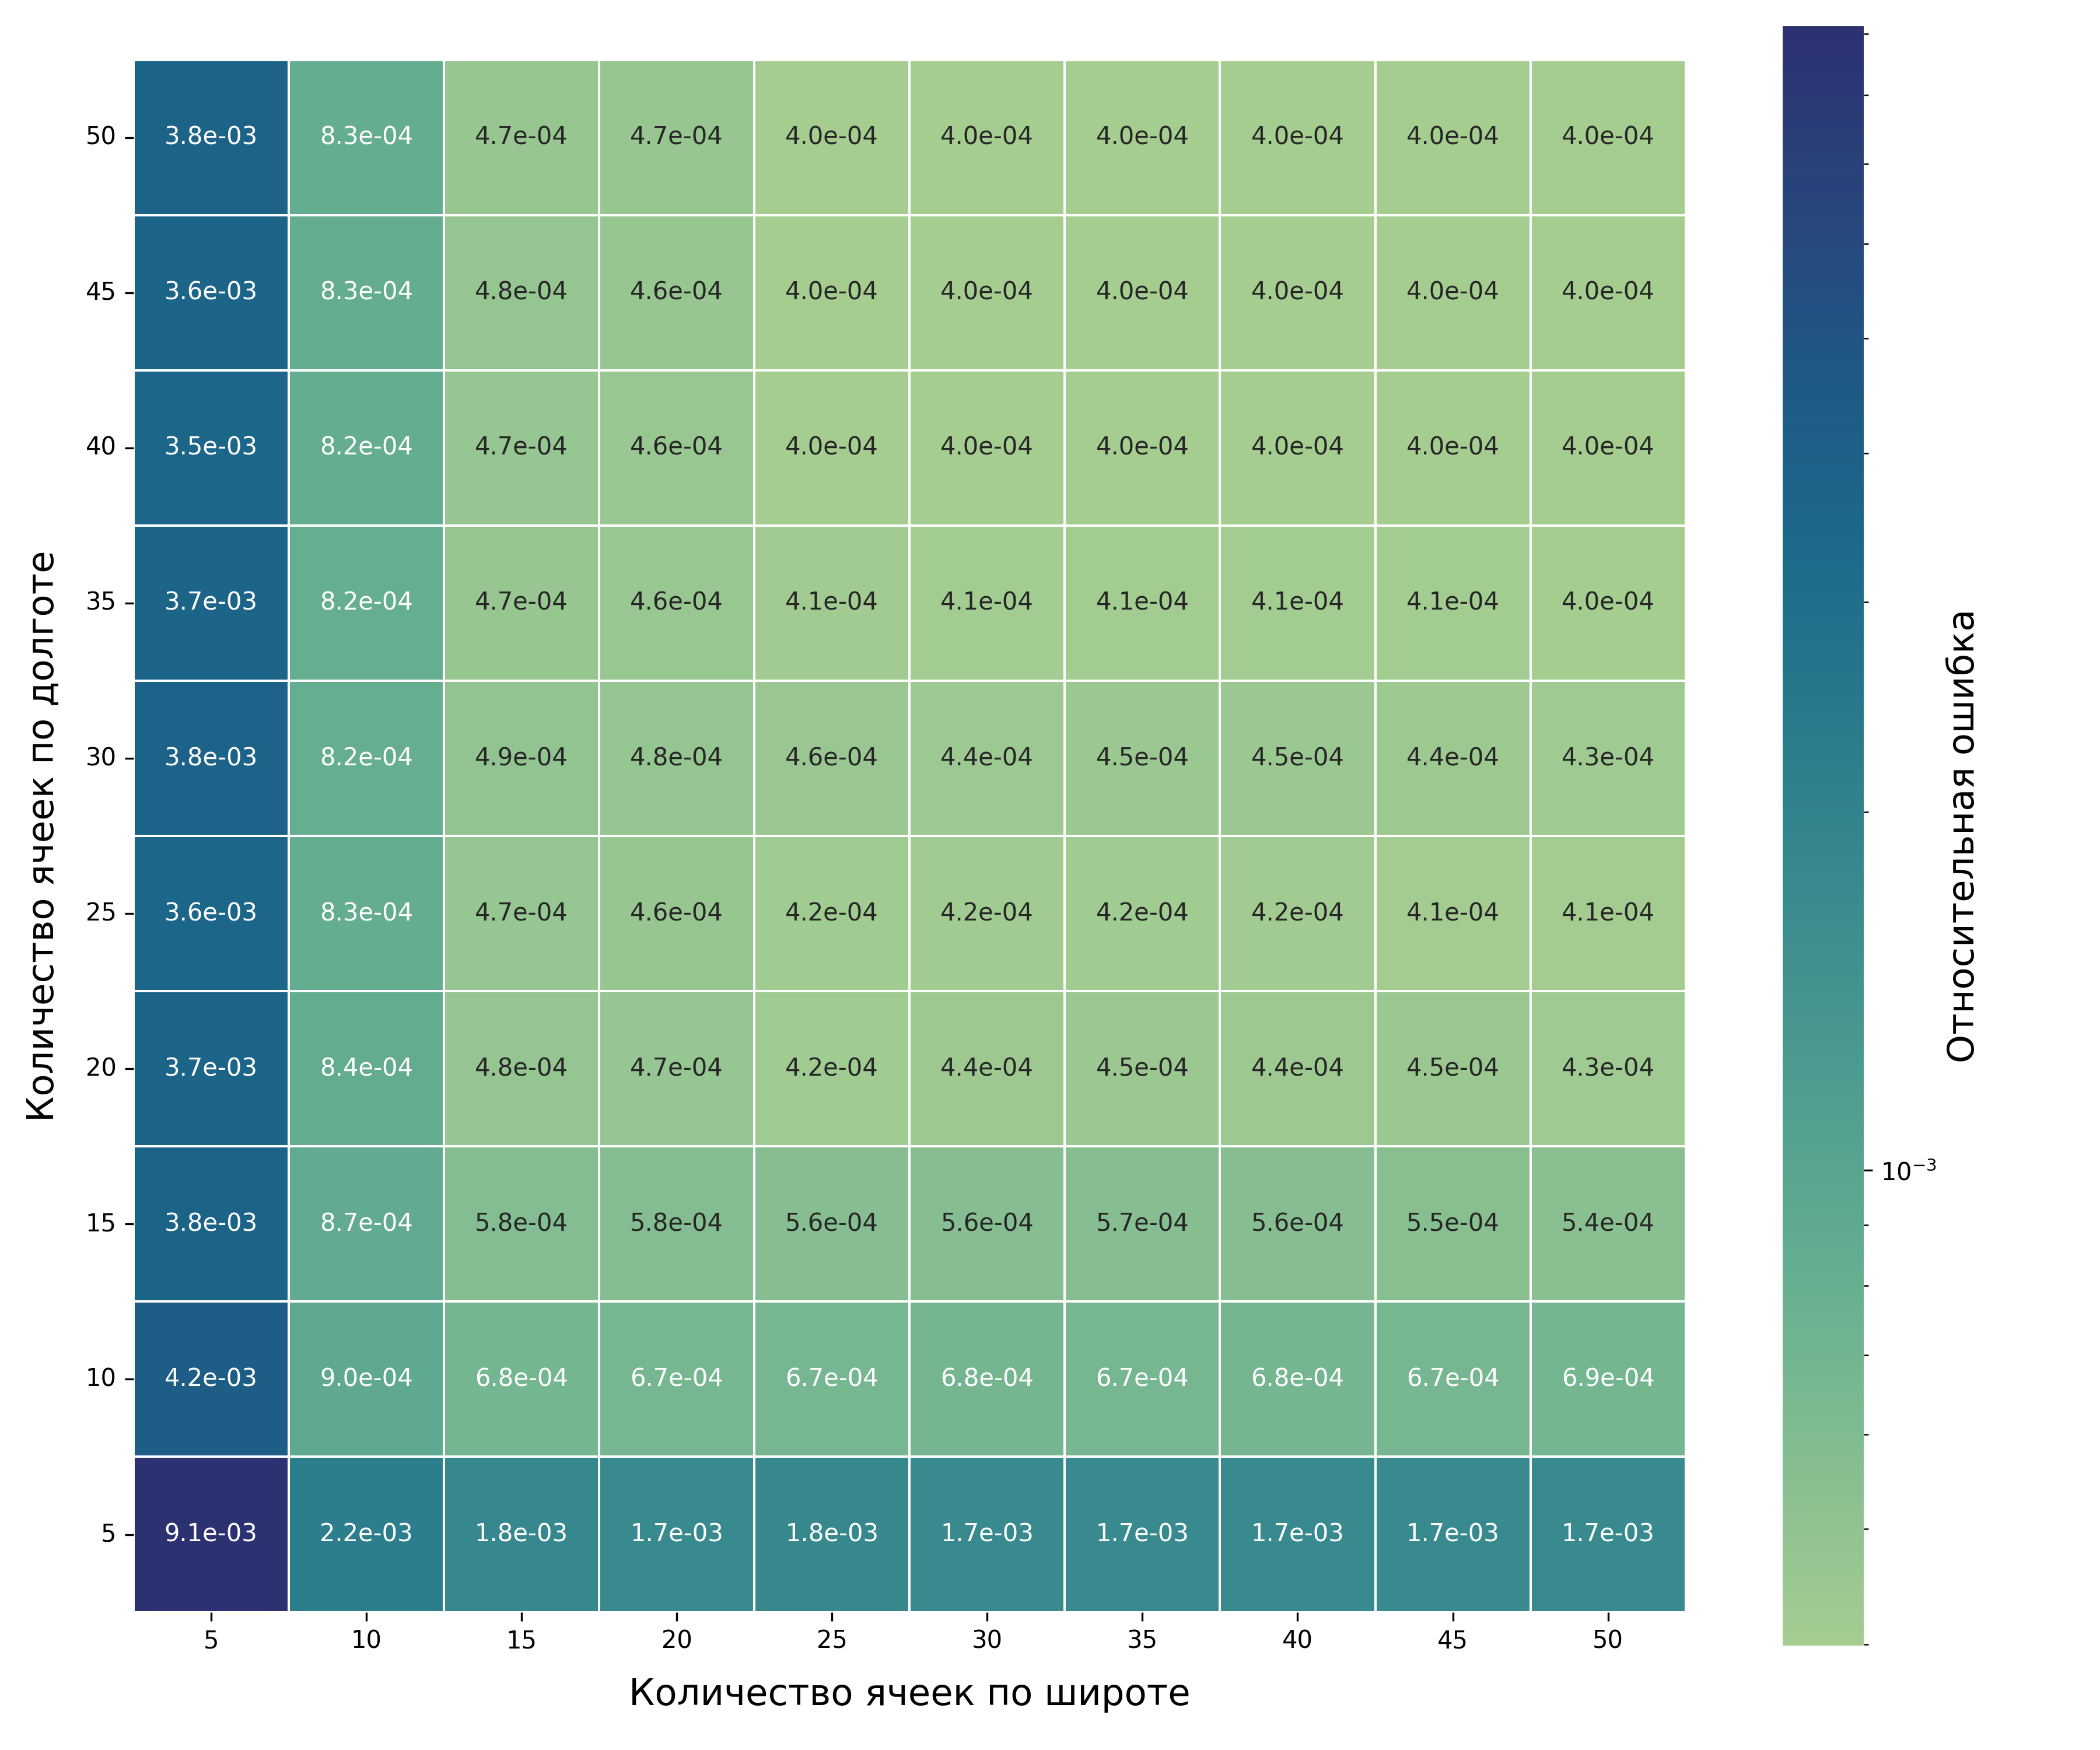
\includegraphics[width=0.85\linewidth]{../images/solution/atmo/2573_heatmap.png}
    \captionof{figure}{Карта ошибок для конфигурации (2, 5, 7, 3)}
    \label{fig:atmo:2573_heatmap}
 \end{figure}

 \begin{figure}[h!]
    \centering
    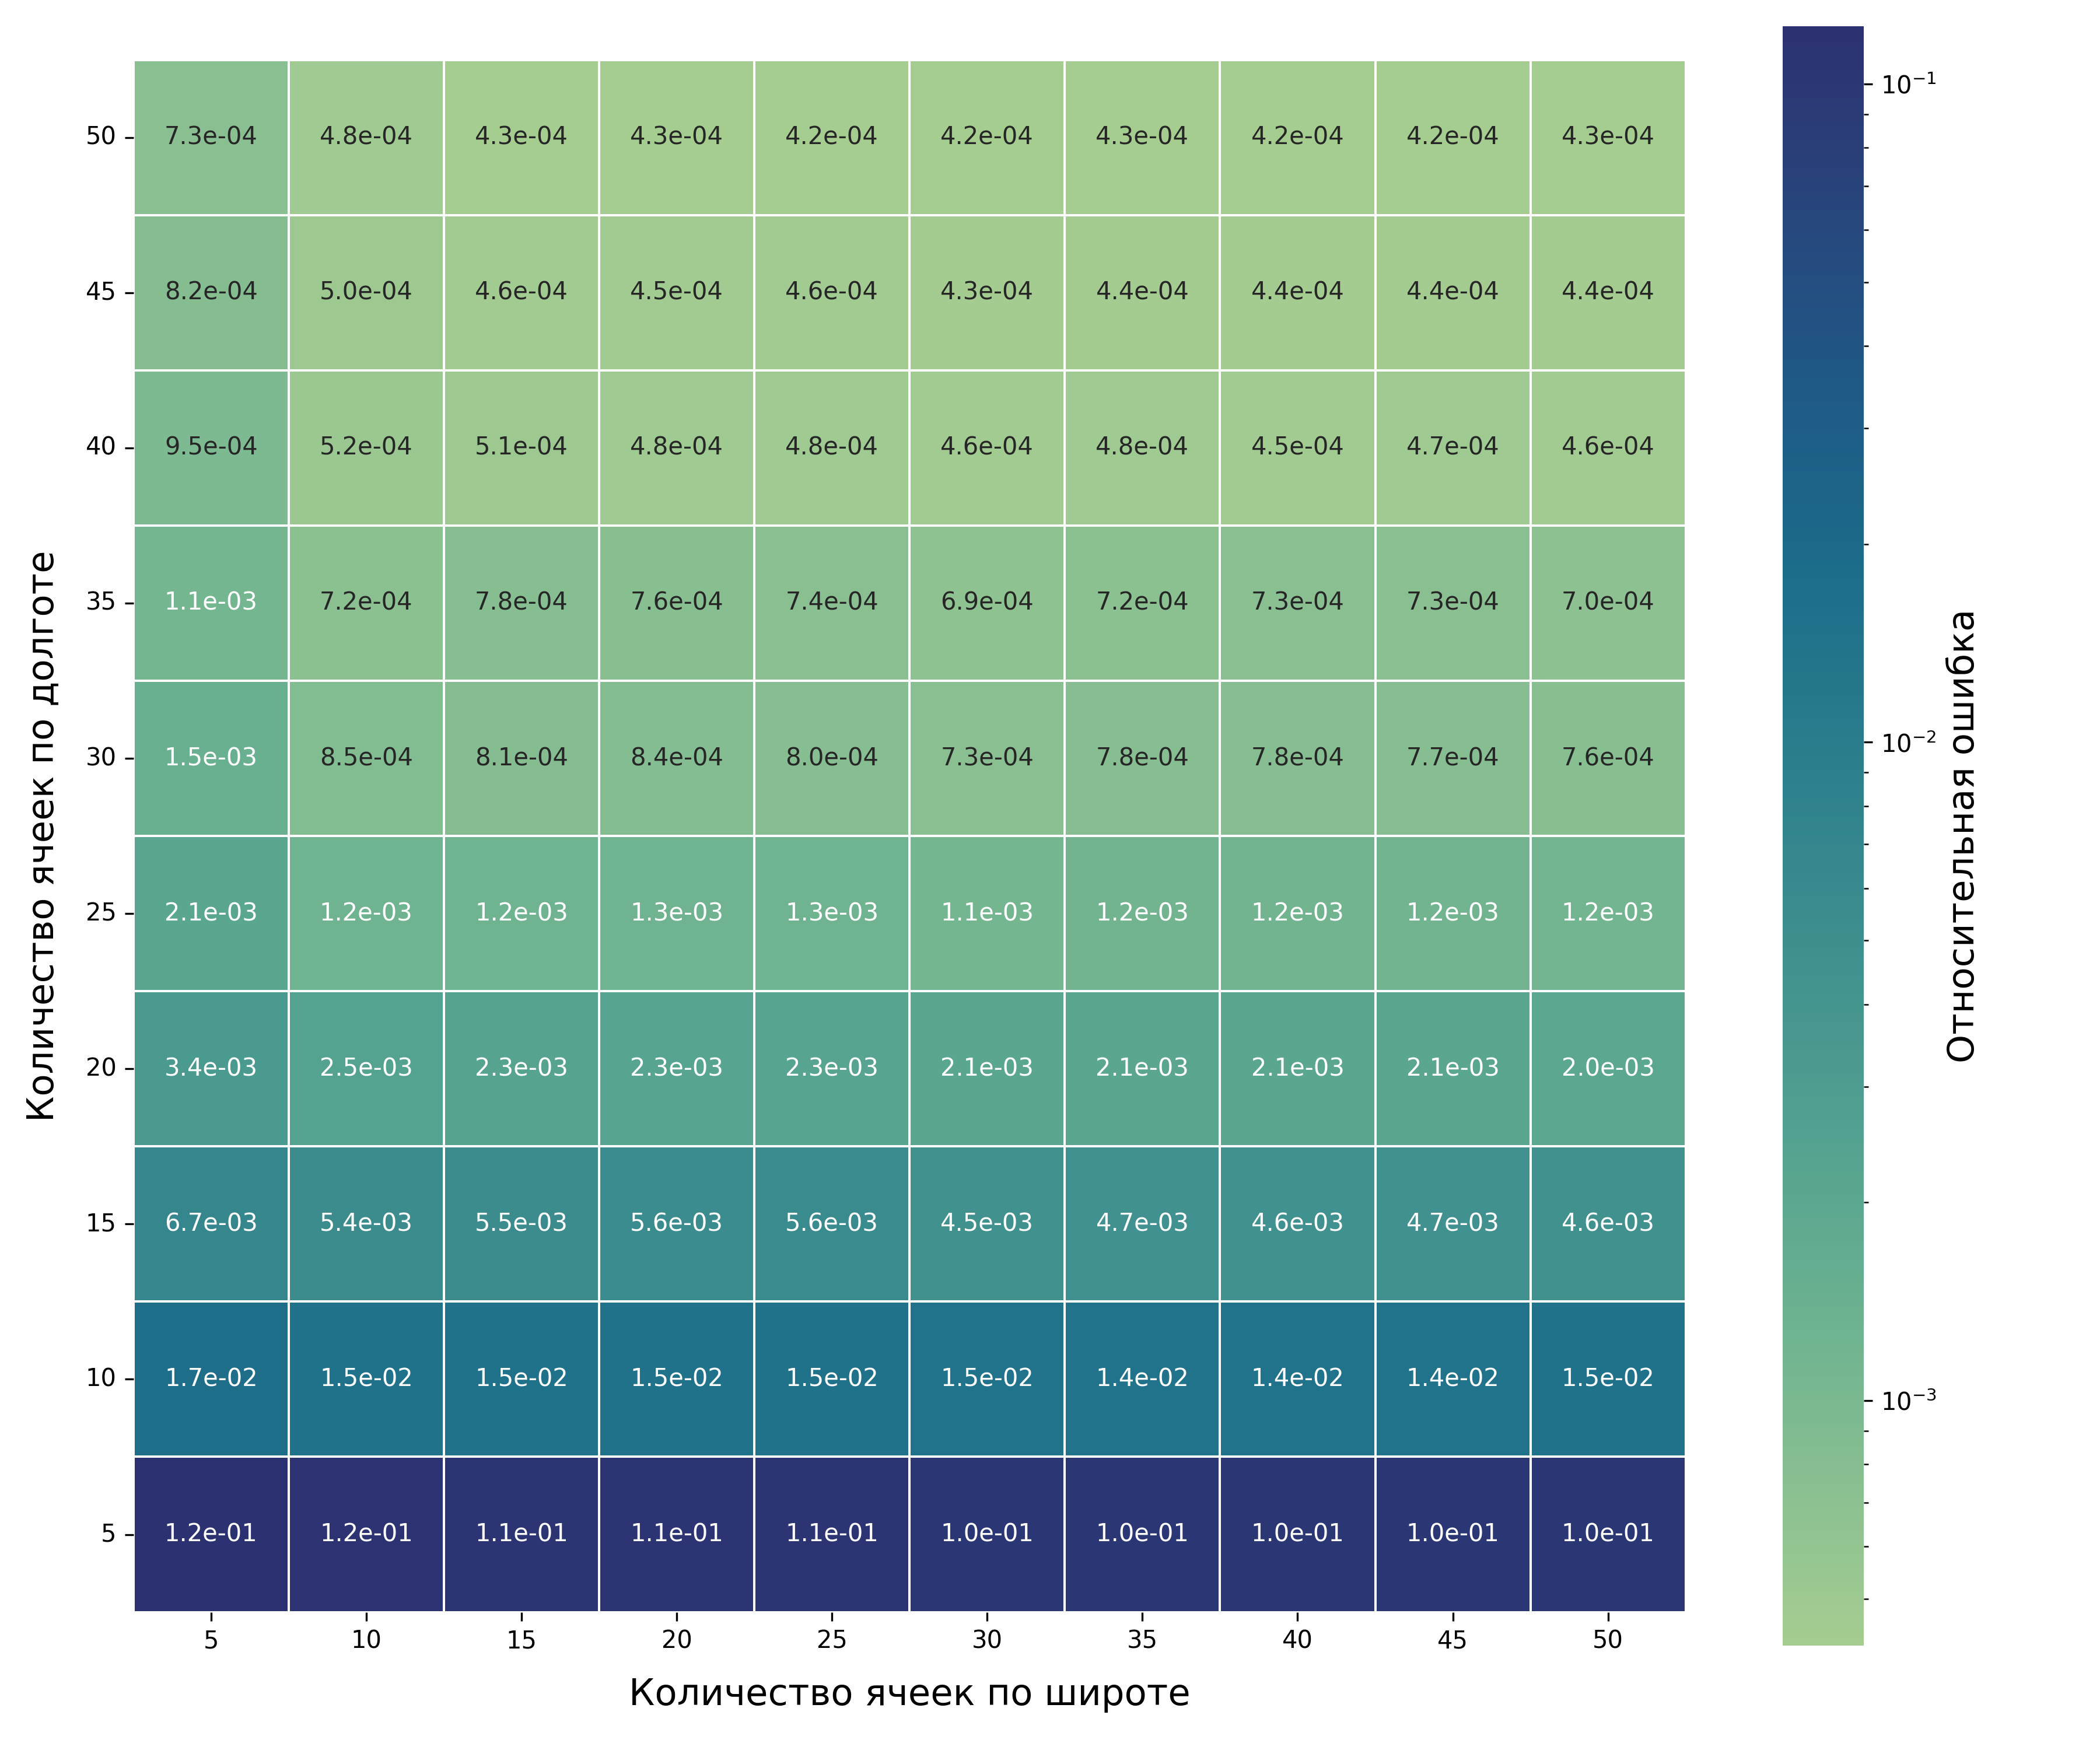
\includegraphics[width=0.85\linewidth]{../images/solution/atmo/2735_heatmap.png}
    \captionof{figure}{Карта ошибок для конфигурации (2, 7, 3, 5)}
    \label{fig:atmo:2735_heatmap}
 \end{figure}

 \begin{figure}[h!]
    \centering
    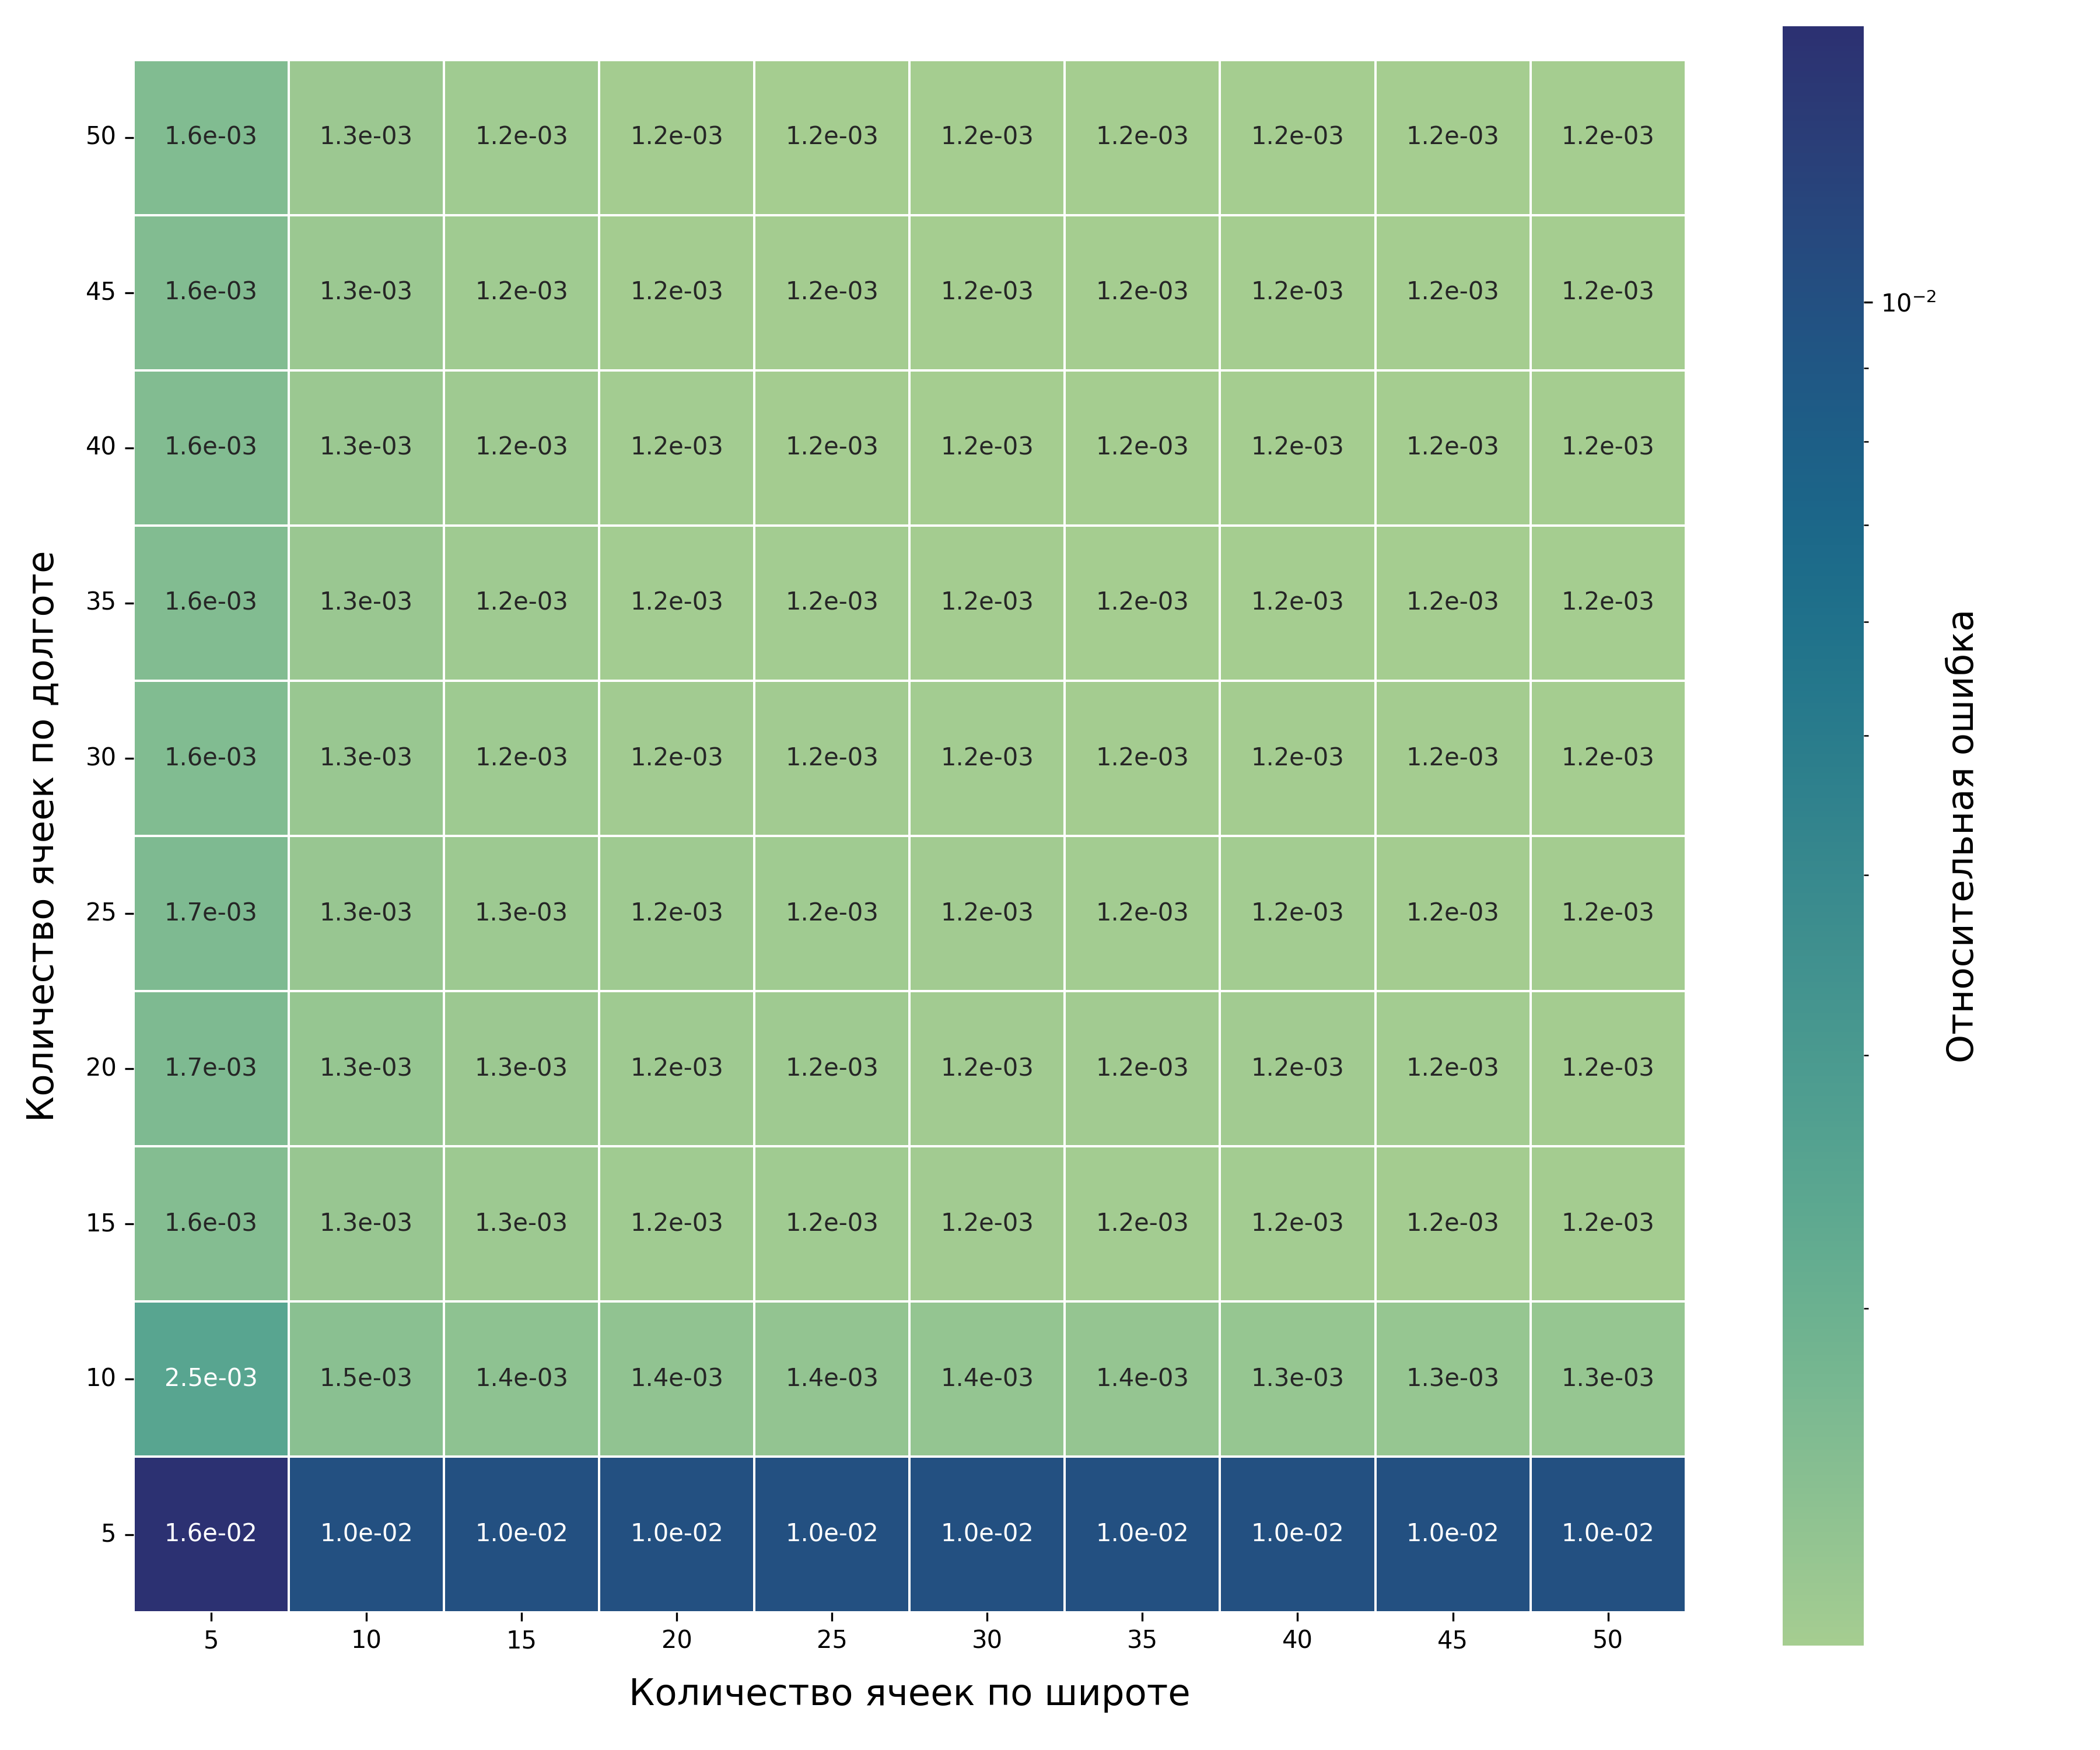
\includegraphics[width=0.85\linewidth]{../images/solution/atmo/2753_heatmap.png}
    \captionof{figure}{Карта ошибок для конфигурации (2, 7, 5, 3)}
    \label{fig:atmo:2753_heatmap}
 \end{figure}

 \begin{figure}[h!]
    \centering
    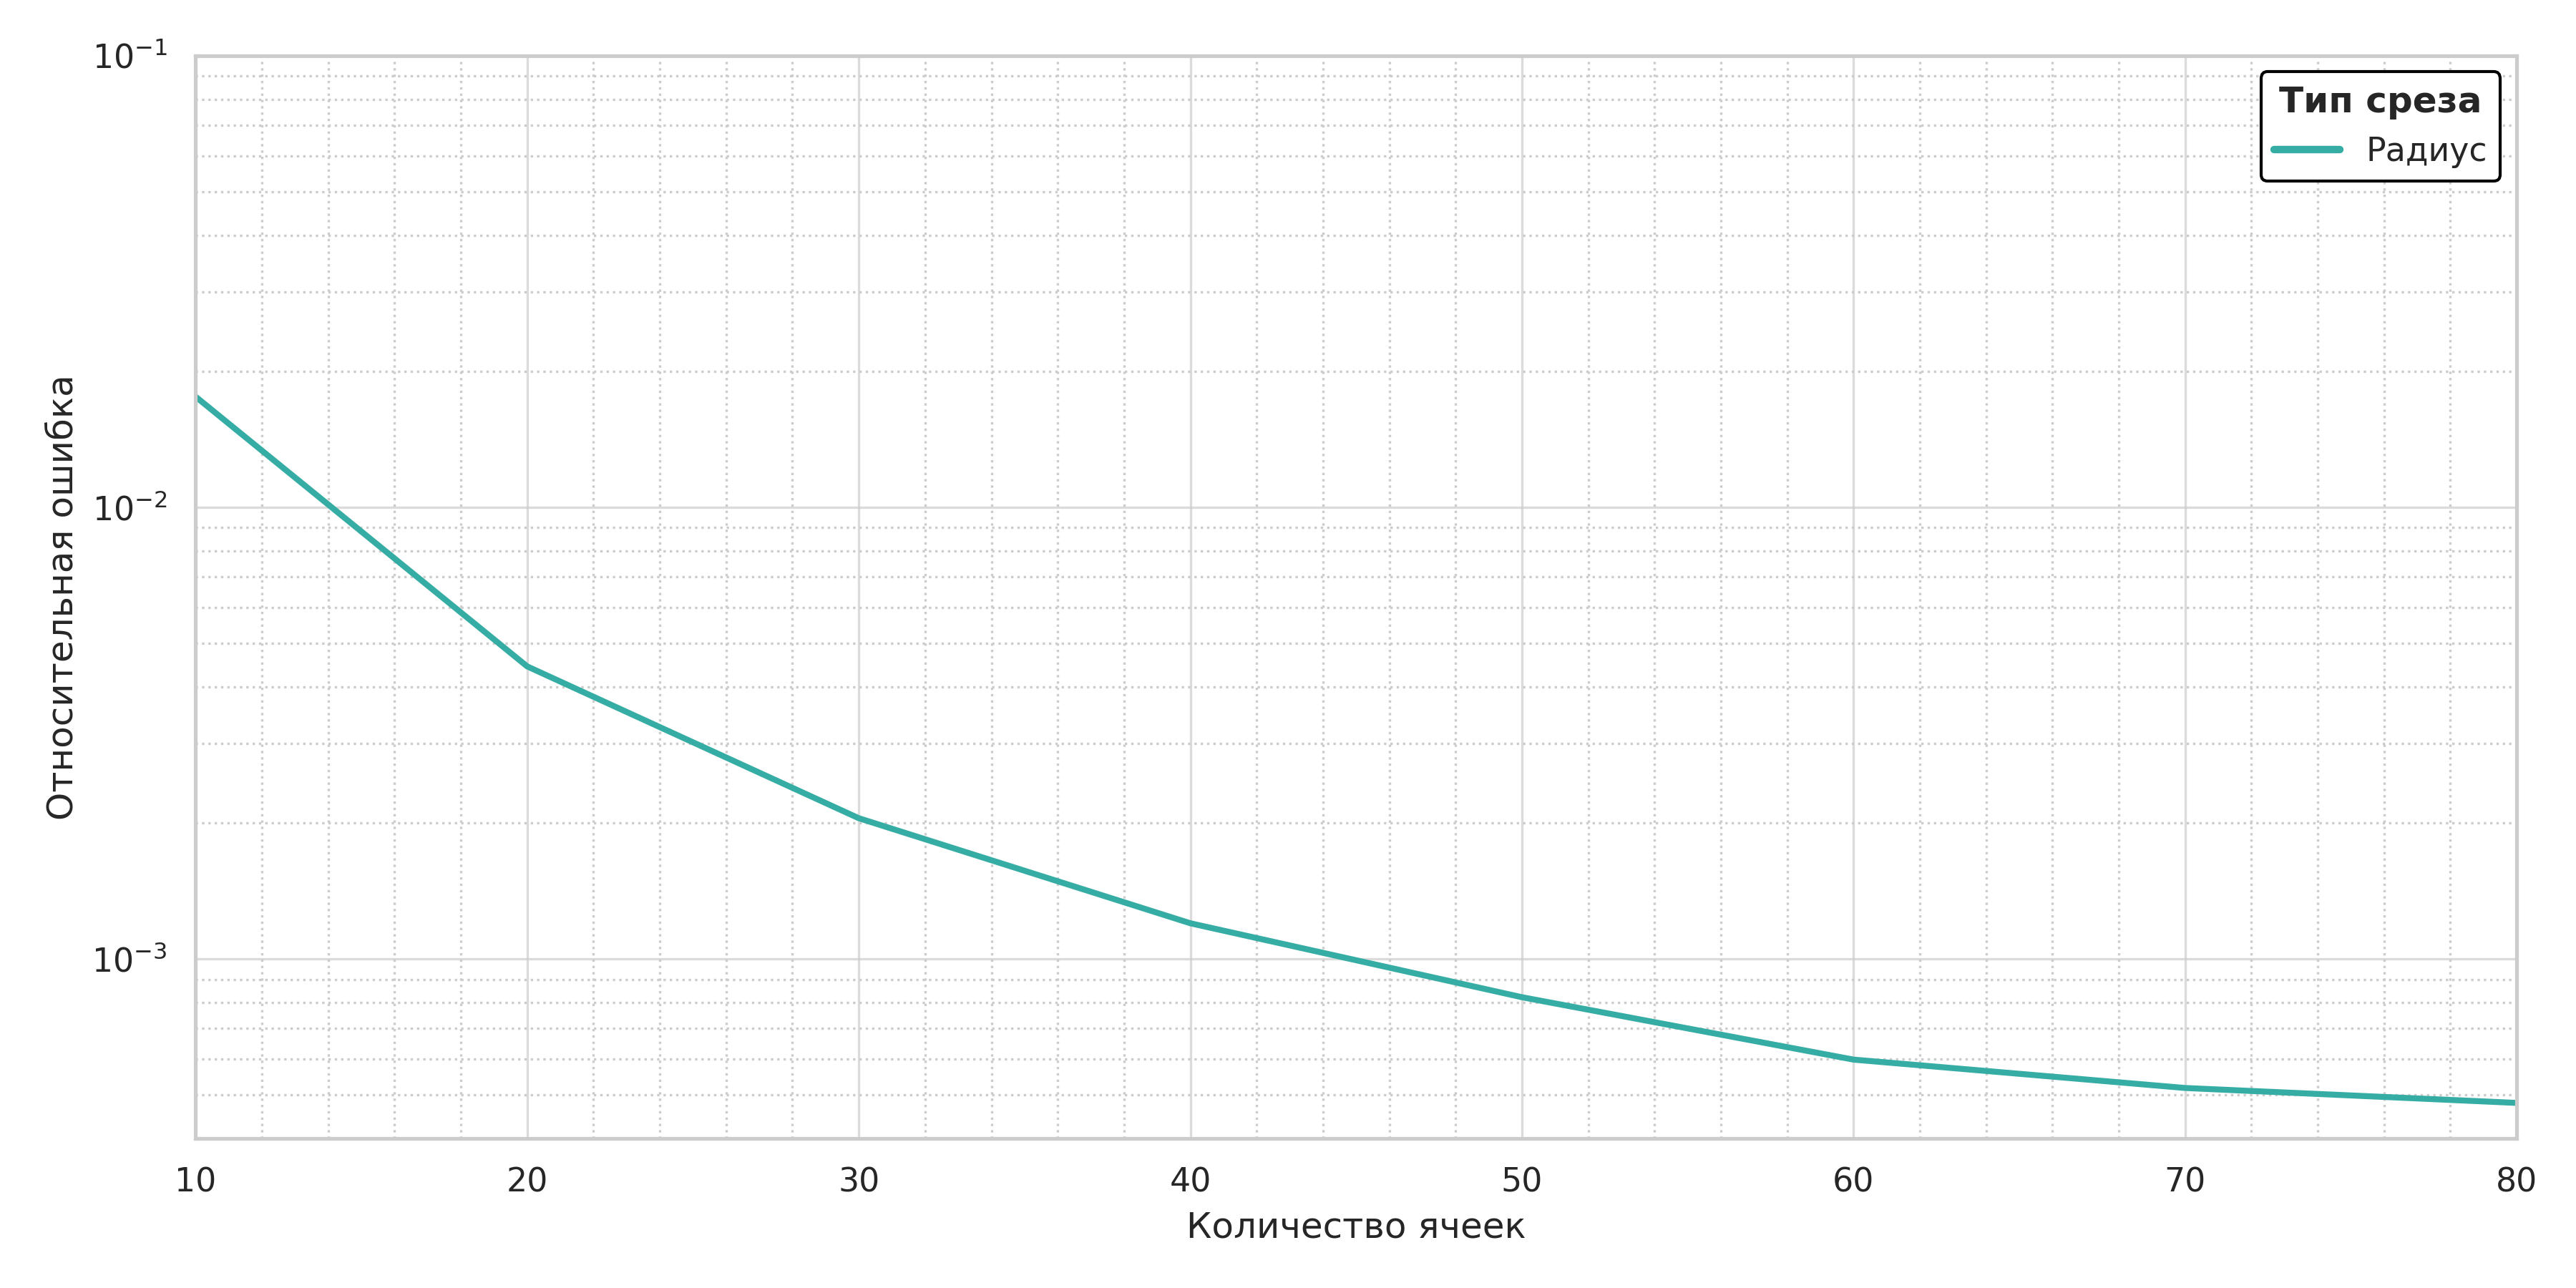
\includegraphics[width=\linewidth]{../images/solution/atmo/2357_rho.png}
    \captionof{figure}{Зависимость ошибки от количества ячеек интерполянта по радиусу для конфигурации (2, 3, 5, 7)}
    \label{fig:atmo:2357_rho}
 \end{figure}

 На картах \ref{fig:atmo:2753_latlon} и \ref{fig:atmo:2753_latlon_abs_err} приведено
 распределение плотности и абсолютной ошибки для интерполянта на высоте 350 километров.
 Использовалась конфигурация (2, 7, 5, 3) с количеством ячеек (65, 50, 50, 50). Темные участки, относящиеся к областям с
 повышенной плотностью, совпадают с участками, на которых интерполяция дает наибольшую абсолютную ошибку.
 В то же время относительная ошибка меняется по области не существенно. Темное пятно в левой
 части графика соответствуют положению, находящемуся под прямыми солнечными лучами.
 Темные полосы на рис. \ref{fig:atmo:2753_latlon_abs_err} возникают на границе ячеек
 по широте и долготе. 

 \begin{figure}[h!]
    \centering
    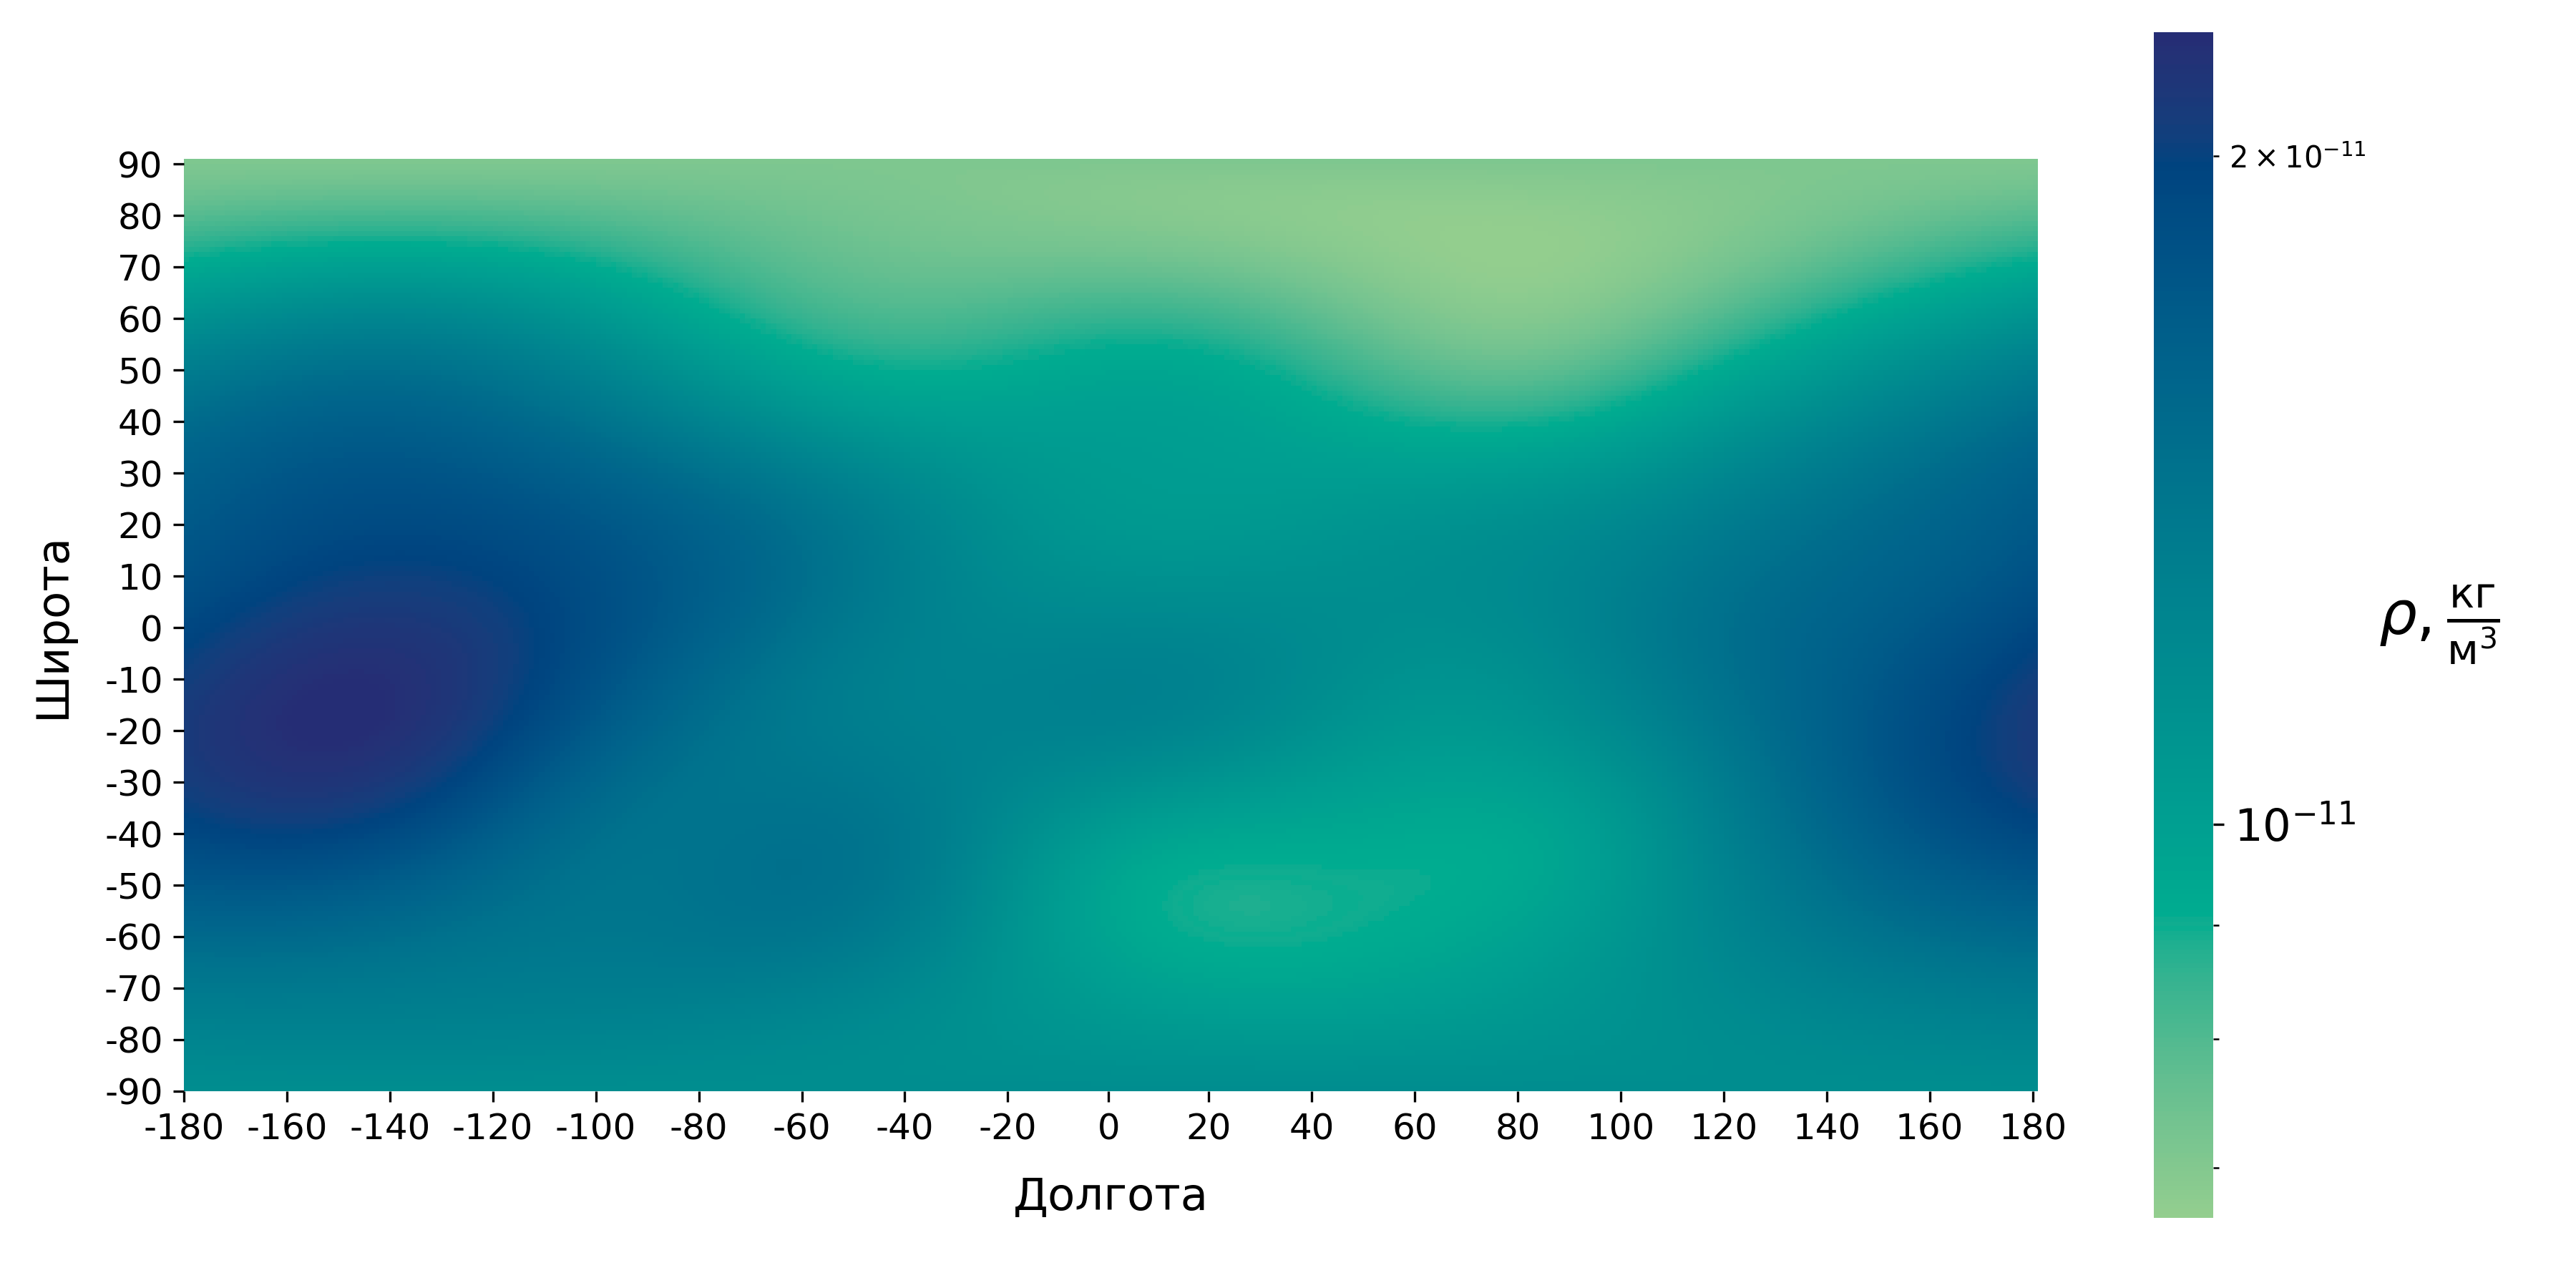
\includegraphics[width=\linewidth]{../images/solution/atmo/2753_latlon_direct_val_heatmap.png}
    \captionof{figure}{Распределение плотности $\rho(\phi, \lambda)$ для конфигурации (2, 7, 5, 3)}
    \label{fig:atmo:2753_latlon}
 \end{figure}

 \begin{figure}[h!]
    \centering
    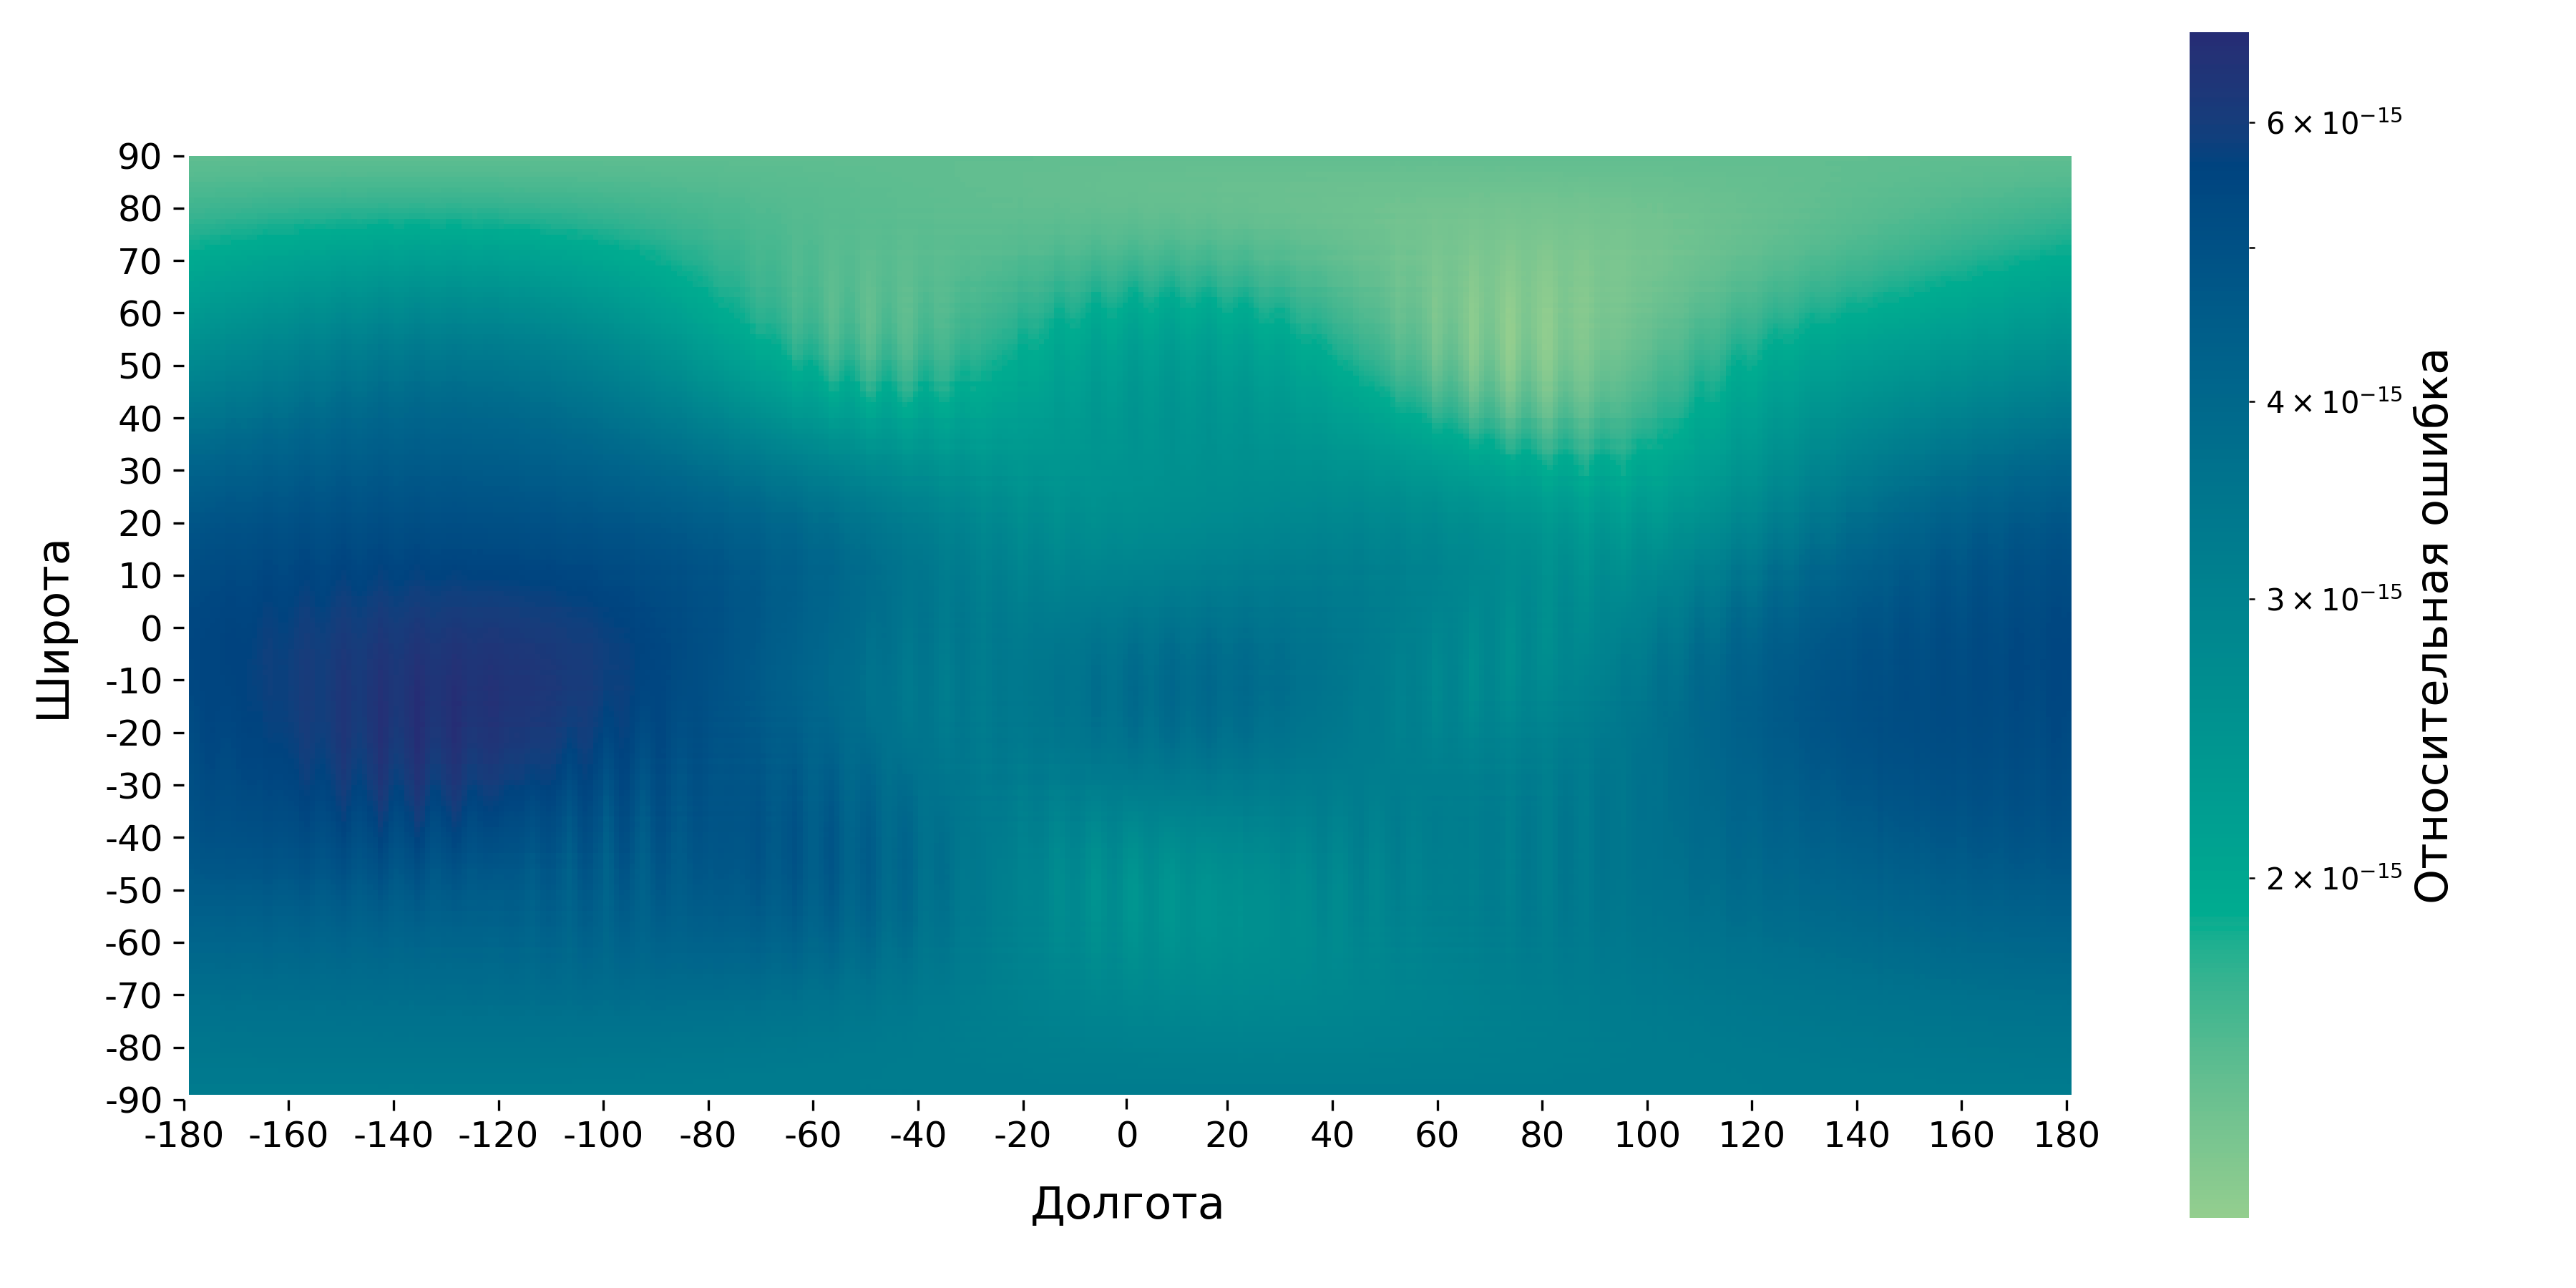
\includegraphics[width=\linewidth]{../images/solution/atmo/2753_latlon_abs_error_heatmap.png}
    \captionof{figure}{Распределение абсолютной ошибки вычисления плотности для конфигурации (2, 7, 5, 3)}
    \label{fig:atmo:2753_latlon_abs_err}
 \end{figure}

 На основе данных о поточечном сравнении для каждой конфигурации были подобраны интерполянты, 
 позволяющие достичь малой ошибки при минимальном размере. 
 Характеристики выбранных интерполянтов представлены в таблице \ref{tab:atmo_propag}.

 Тестирование прогноза с использованием интерполянтов проводилось следующим образом.
 Большая часть космических объектов имеет отношение площади к массе 0.001 -- 0.1,
 поэтому в тестах этот параметр был зафиксирован на величине 0.1. Исходя из дополнительных
 рассчетов, зависимость ошибки прогноза от данного параметра близка к линейной. Поэтому
 ошибку для объектов с большим соотношением площади к массе (например, у пленок) 
 можно легко получить.
 Рассмотрено более 5000 тысяч околоземных орбит с высотами от 350 до 800 километров. 
 Гравитация учитывалась по модели EGM2008 с 64 гармониками. Вычисления проводились
 с помощью явного метода Рунге--Кутты 7-го порядка, а период интегрирования составил 1 день.
 Сначала траектория вычислялась напрямую, затем с интерполяцией плотности атмосферы.
 За ошибку принята разность между двумя прогнозами. Для наглядности на рис. 
 \ref{fig:atmo:2357_propag_1} -- \ref{fig:atmo:2735_propag}
 приведена максимальная ошибка по высотам орбит с интервалом 50--100 км.

 На исследованных интерполянтах ошибки в пределах 10 метра удается достичь на высотах
 от 400 километров. Такую точность можно считать достаточной при построении НОО.

 Как отмечалось ранее, ускорение интерполянта главным образом зависит от скорости
 вычисления линейной комбинации произведений полиномов Чебышева в ячейке. 
 Эта скорость определяется максимальным порядком каждого полинома. Поэтому каждая
 рассмотренная конфигурация дает примерно одно и то же ускорение. Небольшие различия
 могут быть вызваны объемом интерполянта. Коэффициенты интерполяции во время исполнения
 программы хранятся в оперативной памяти. Эффективность работы памяти, 
 т. е. скорость доступа к ее участку, уменьшается на больших данных. В то же время
 такое замедление не критично, так как качественно не меняет степень ускорения.

 Скорость вычисления плотности атмосферы с интерполянтом выросла в среднем в 17 раз.
 Минимальное ускорение достигалось на больших интерполянтах и равнялось 9. Для избранных
 интерполянтов ускорение варьировалось от 13 до 14. Таким образом, был достигнут
 уровень ресурсоемкости вычисления гравитационного потенциала с интерполяцией.

 \begin{table}[h!]
    \caption{Результаты тестирования выбранных интерполянтов}
    \centering
    \renewcommand{\arraystretch}{1.5}
    \begin{tabular}{|l|l|l|l|l|}
    \hline
    Конфигурация & Количество ячеек & \begin{tabular}[c]{@{}c@{}}Относительная \\ ошибка, \%\end{tabular} & \begin{tabular}[c]{@{}c@{}}Максимальная \\ ошибка прогноза, м\end{tabular} & Размер, ГБ \\ \hline
    (2, 3, 5, 7) & (65, 50, 25, 20) & 0.045                                                               & 12.2                                                                       & 0.97       \\ \hline
    (2, 3, 5, 7) & (65, 45, 35, 20) & 0.041                                                               & 12.3                                                                       & 1.22       \\ \hline
    (2, 3, 7, 5) & (65, 45, 15, 35) & 0.044                                                               & 11.8                                                                       & 0.91       \\ \hline
    (2, 5, 3, 7) & (65, 25, 50, 20) & 0.044                                                               & 12.3                                                                       & 0.97       \\ \hline
    (2, 5, 7, 3) & (65, 25, 20, 50) & 0.042                                                               & 12.6                                                                       & 0.97       \\ \hline
    (2, 7, 3, 5) & (65, 15, 45, 40) & 0.044                                                            & 12.2                                                                       & 1.05       \\ \hline
    \end{tabular}
    \label{tab:atmo_propag}   
\end{table}

\begin{figure}[htbp]
    \centering
    
    % Первая строка
    \begin{subfigure}[b]{0.48\textwidth}
        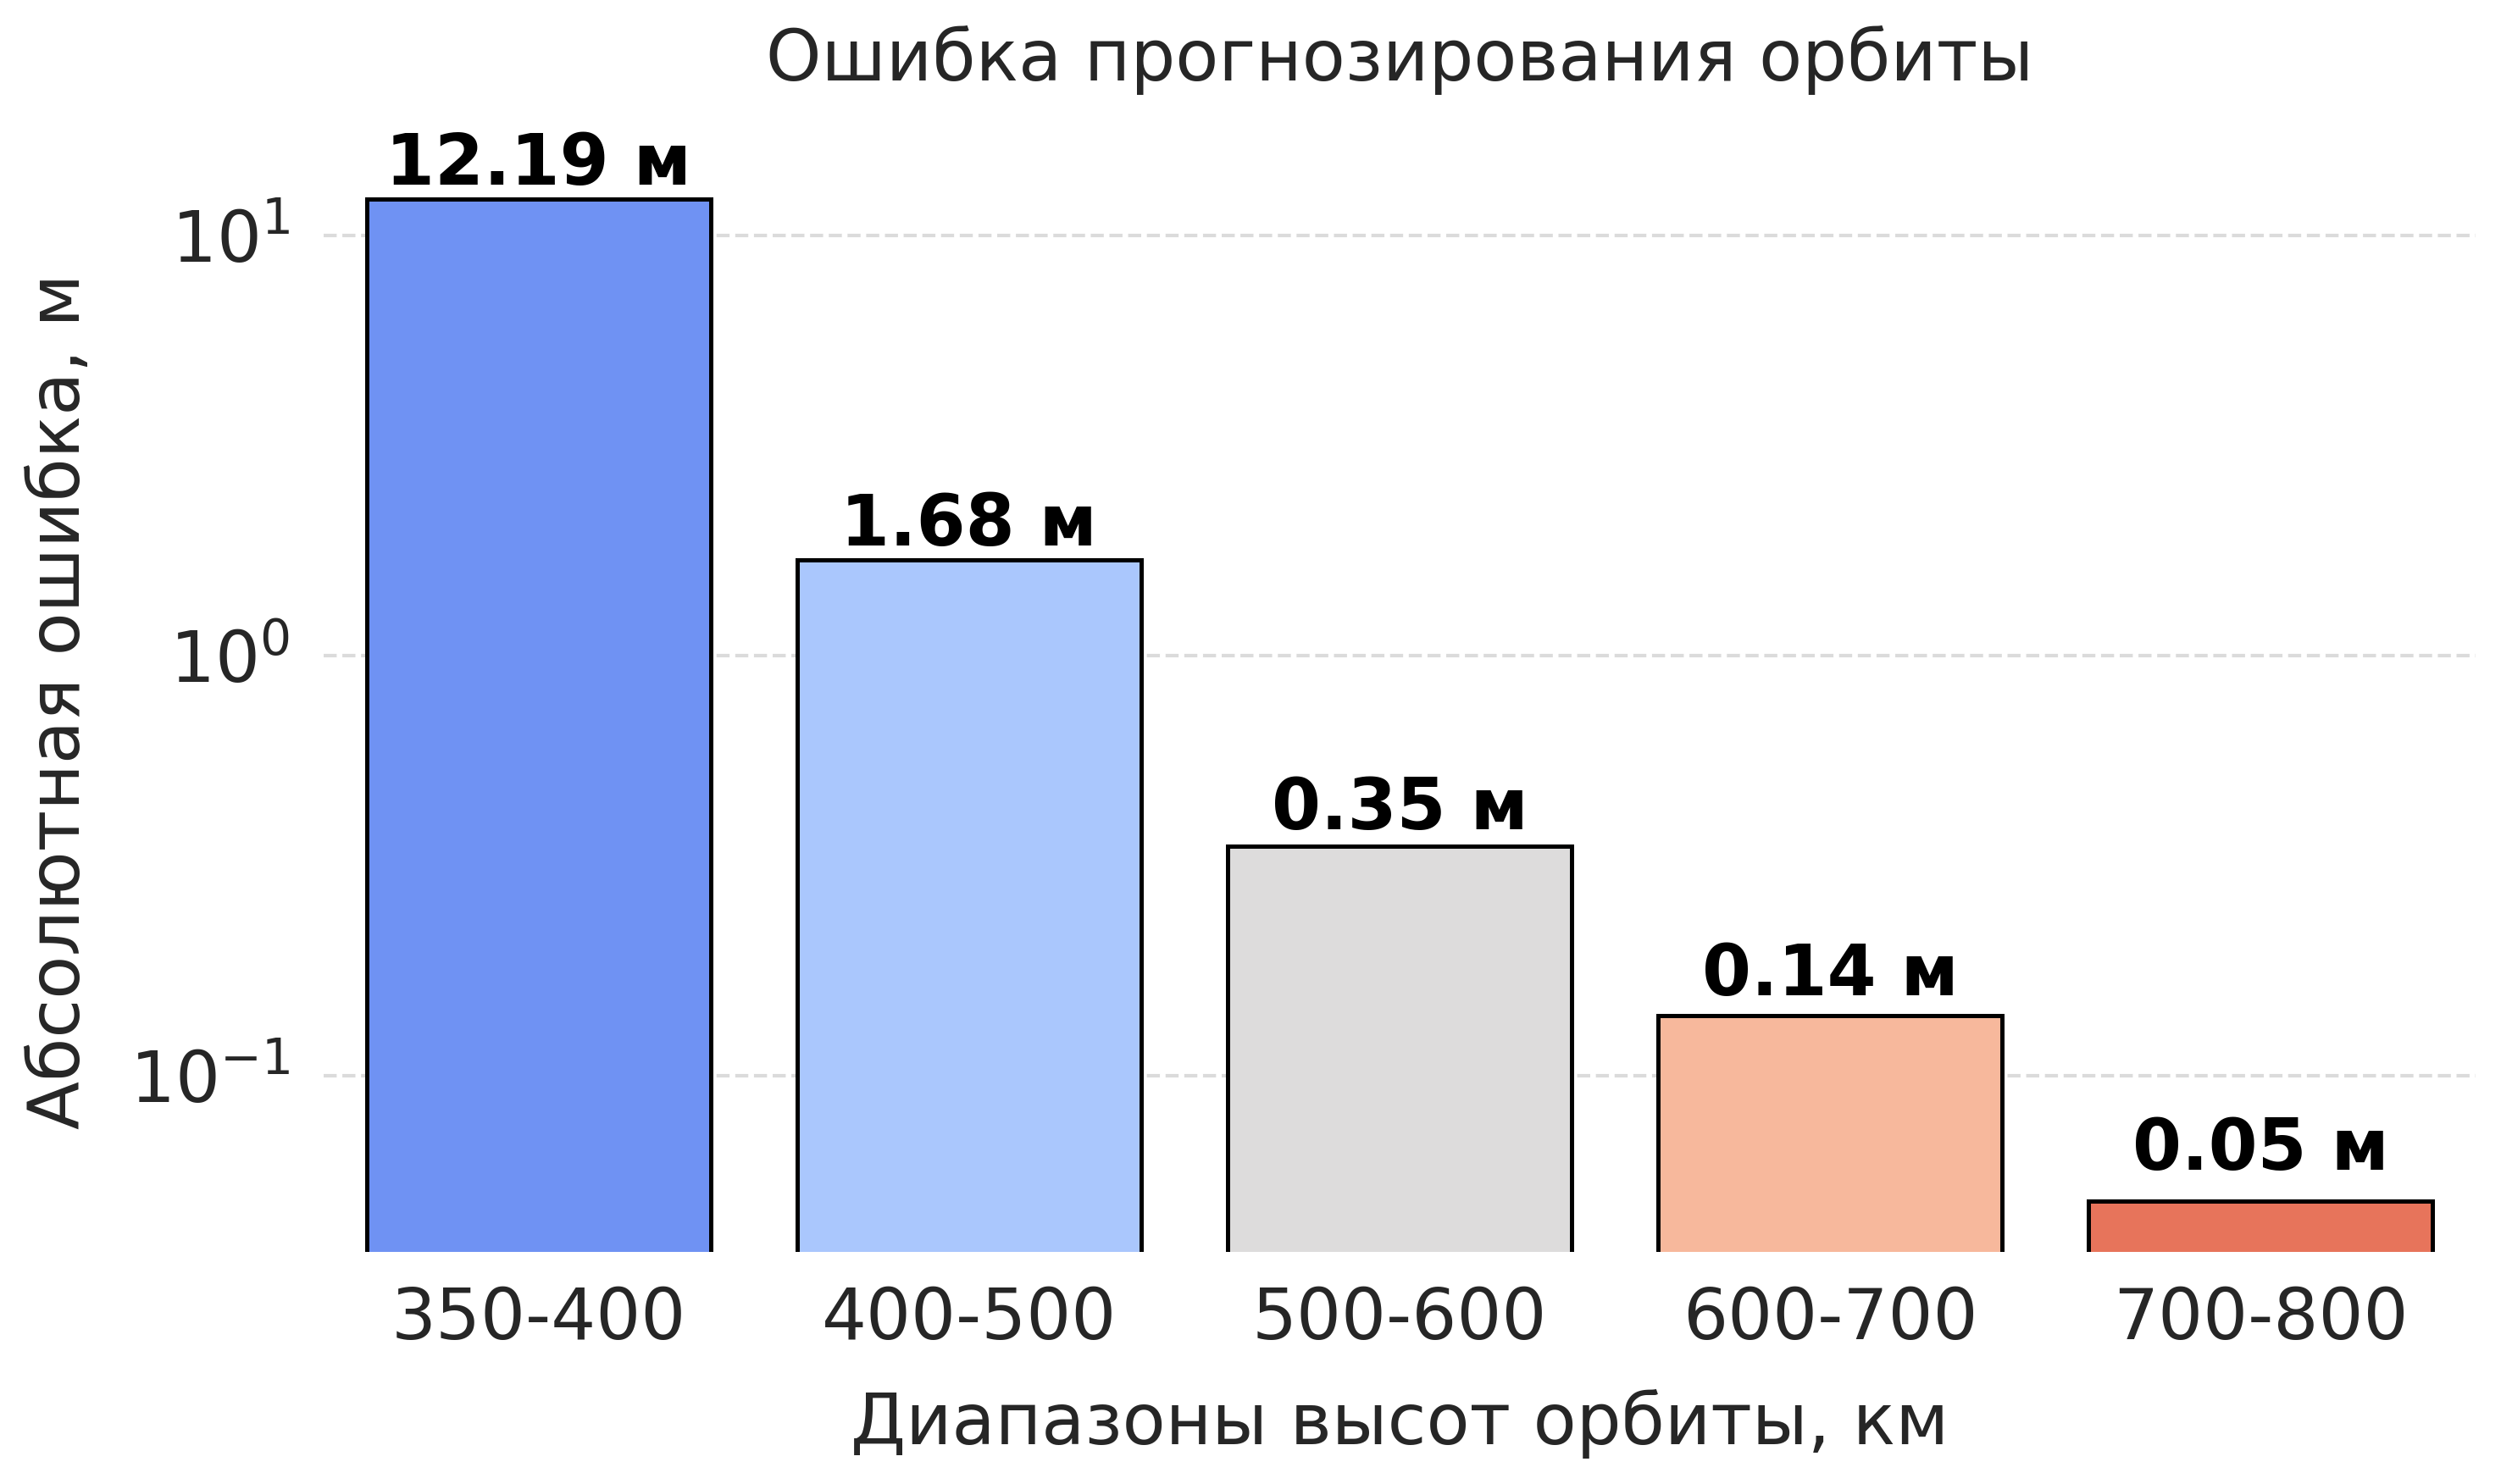
\includegraphics[width=\linewidth]{../images/solution/atmo/propagation/2357_1.png}
        \caption{Конфигурация (2, 3, 5, 7),
        количество ячеек (65, 50, 25, 20)}
        \label{fig:atmo:2357_propag_1}
    \end{subfigure}
    \hfill
    \begin{subfigure}[b]{0.48\textwidth}
        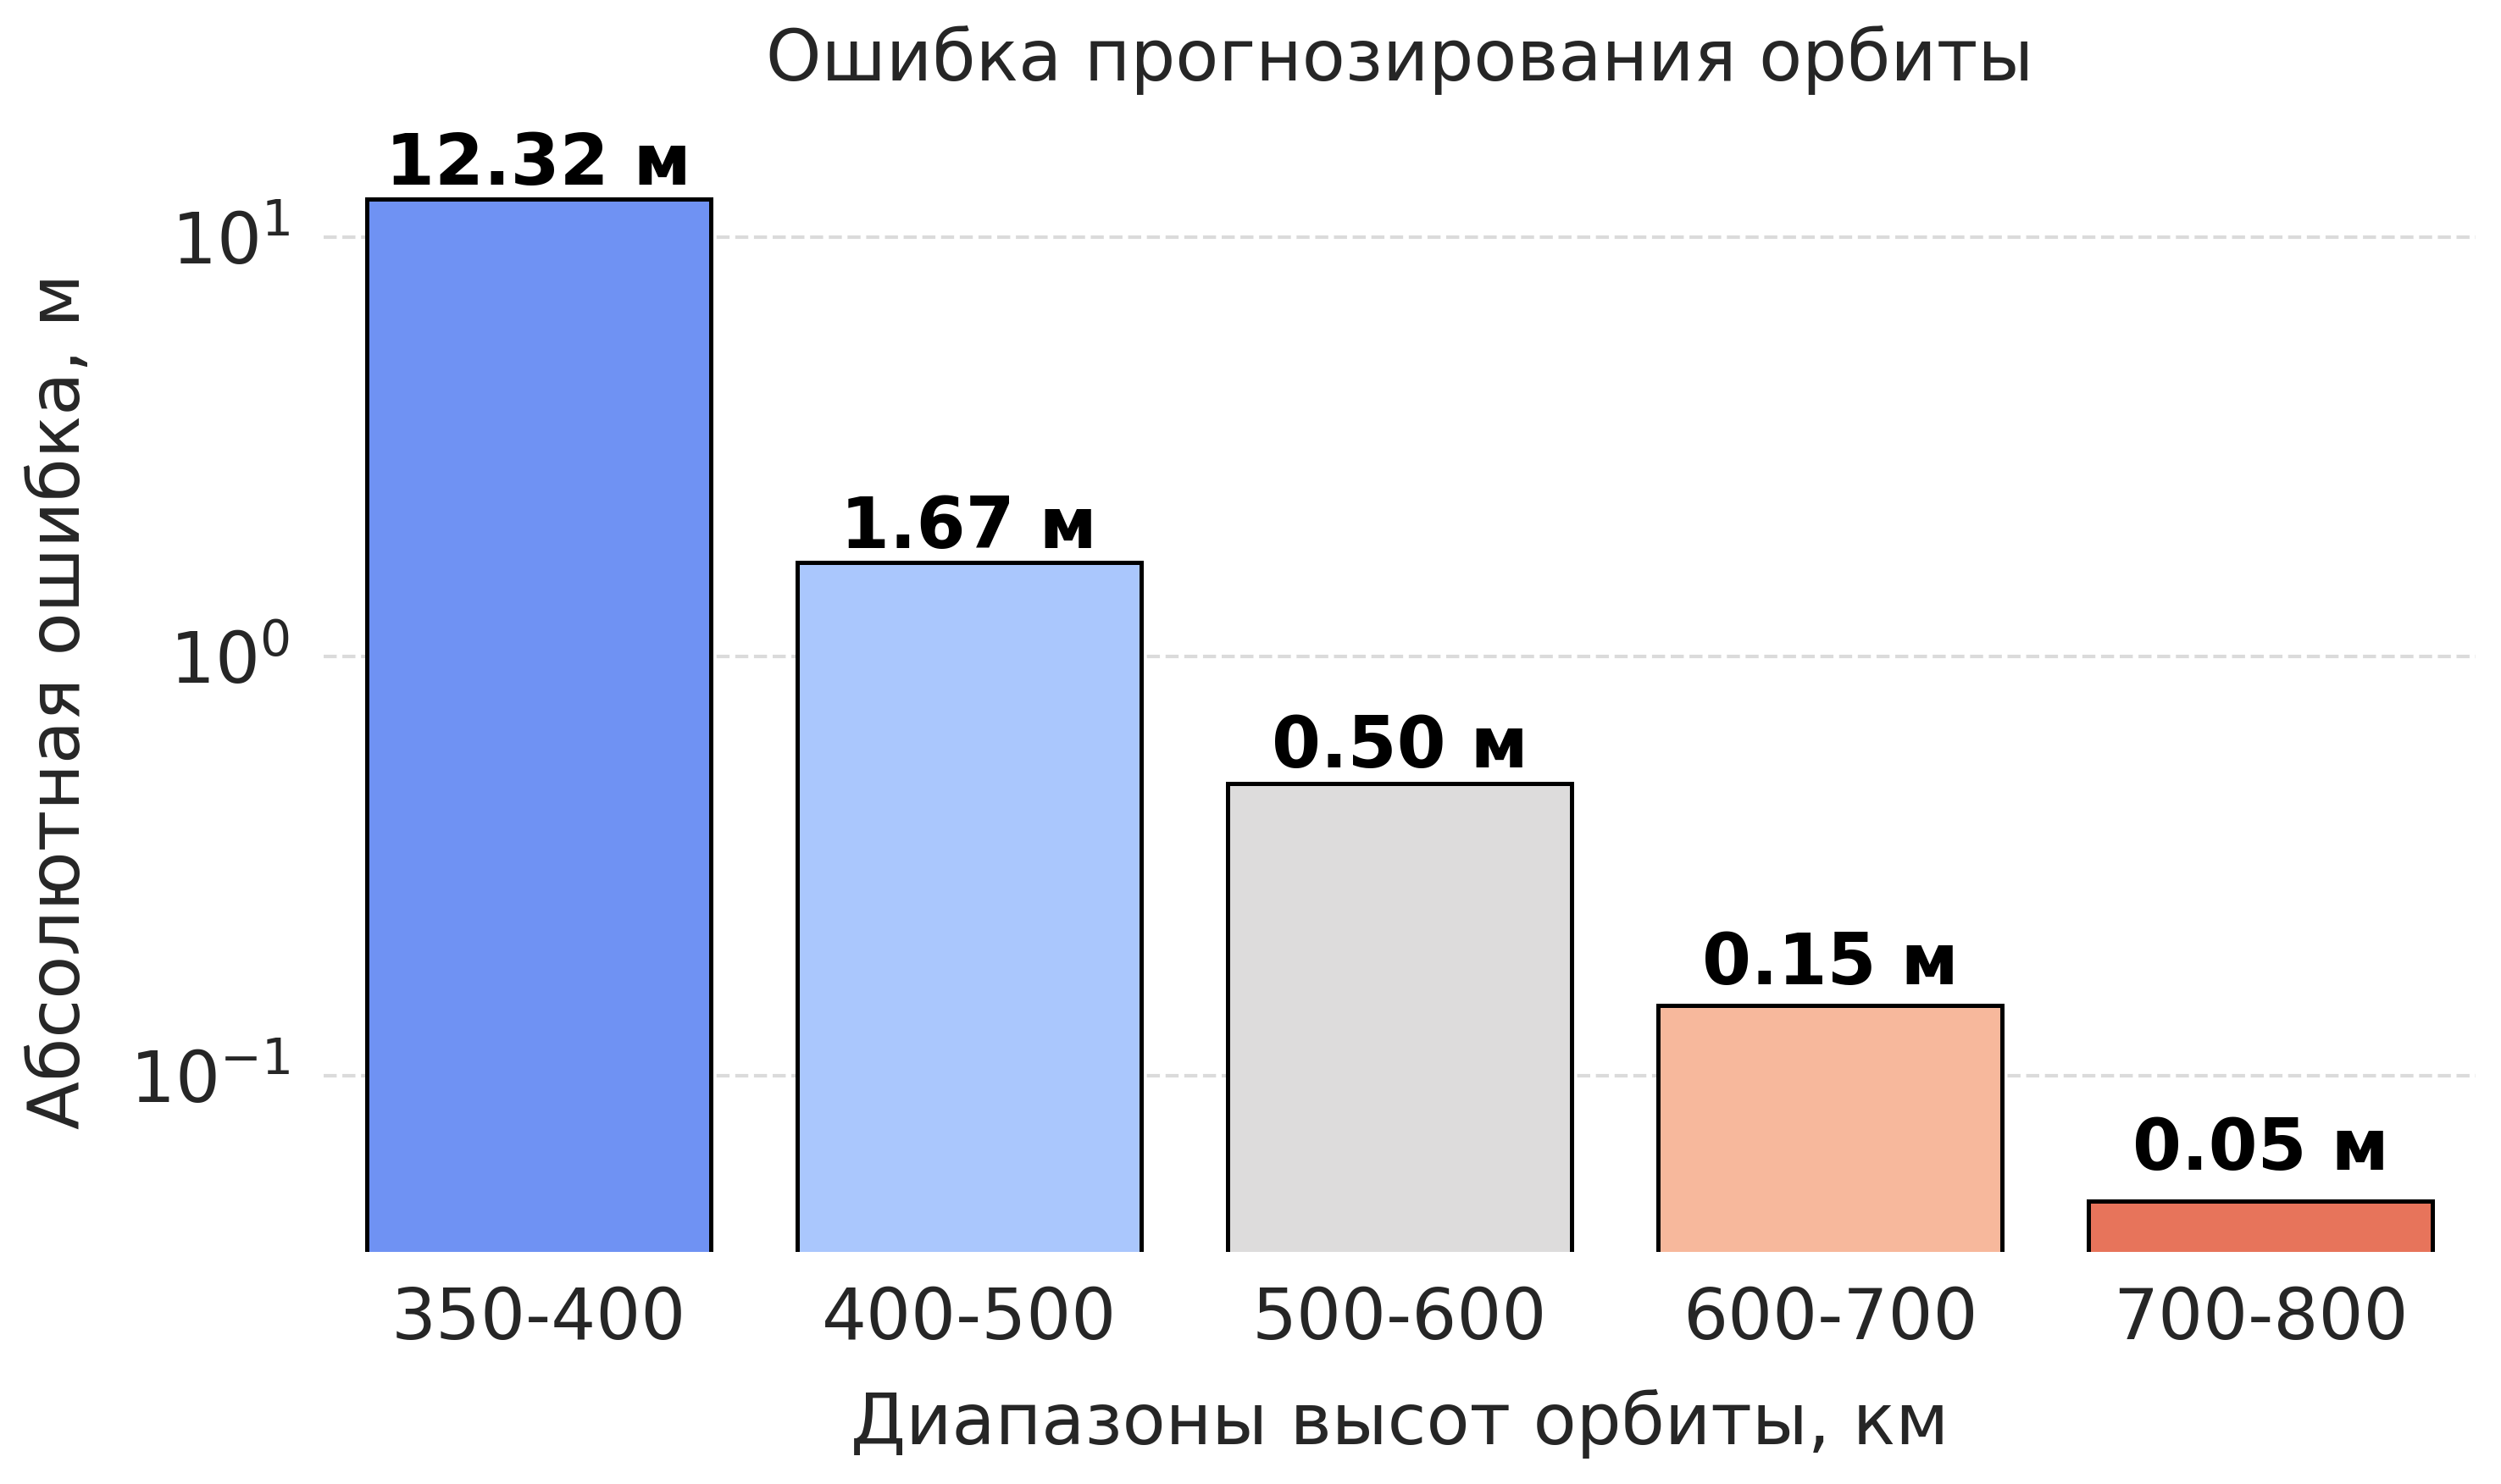
\includegraphics[width=\linewidth]{../images/solution/atmo/propagation/2357_2.png}
        \caption{Конфигурация (2, 3, 5, 7),
        количество ячеек (65, 45, 35, 20)}
        \label{fig:atmo:2357_propag_2}
    \end{subfigure}
    
    \vspace{0.5cm} % Вертикальный отступ между строками
    
    % Вторая строка
    \begin{subfigure}[b]{0.48\textwidth}
        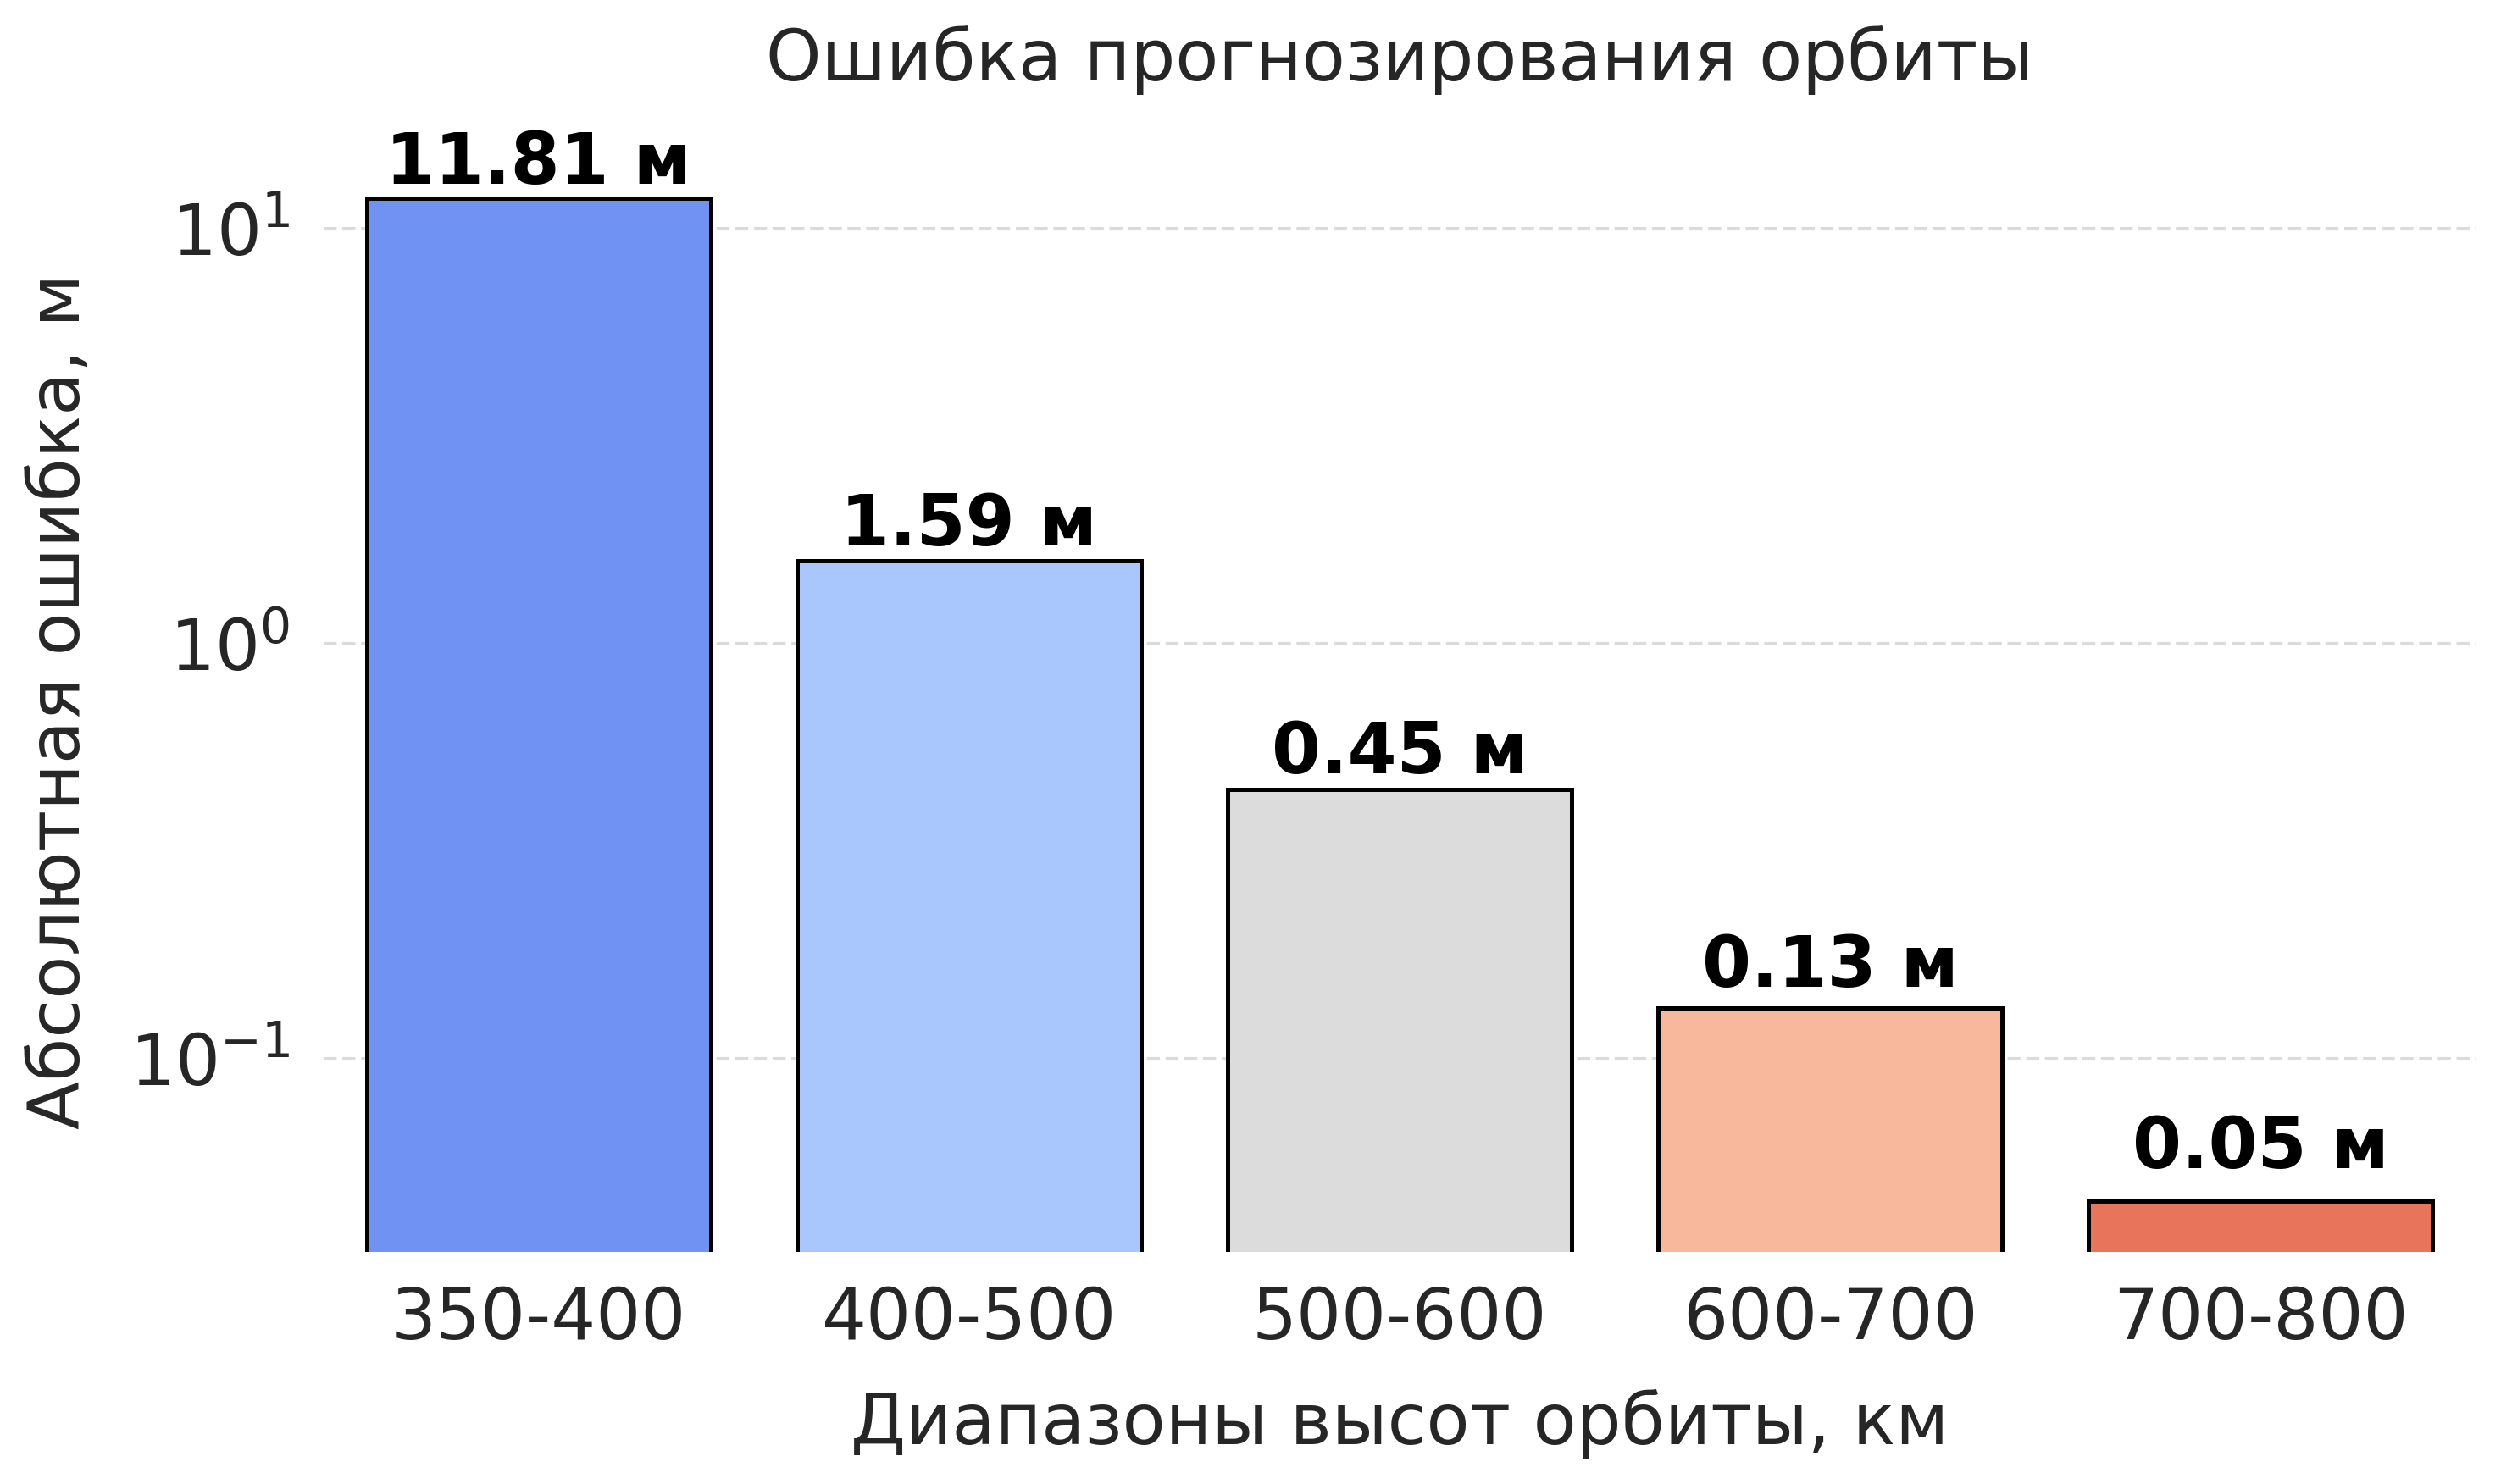
\includegraphics[width=\linewidth]{../images/solution/atmo/propagation/2375.png}
        \caption{Конфигурация (2, 3, 7, 5),
        количество ячеек (65, 45, 15, 35)}
        \label{fig:atmo:2375_propag}
    \end{subfigure}
    \hfill
    \begin{subfigure}[b]{0.48\textwidth}
        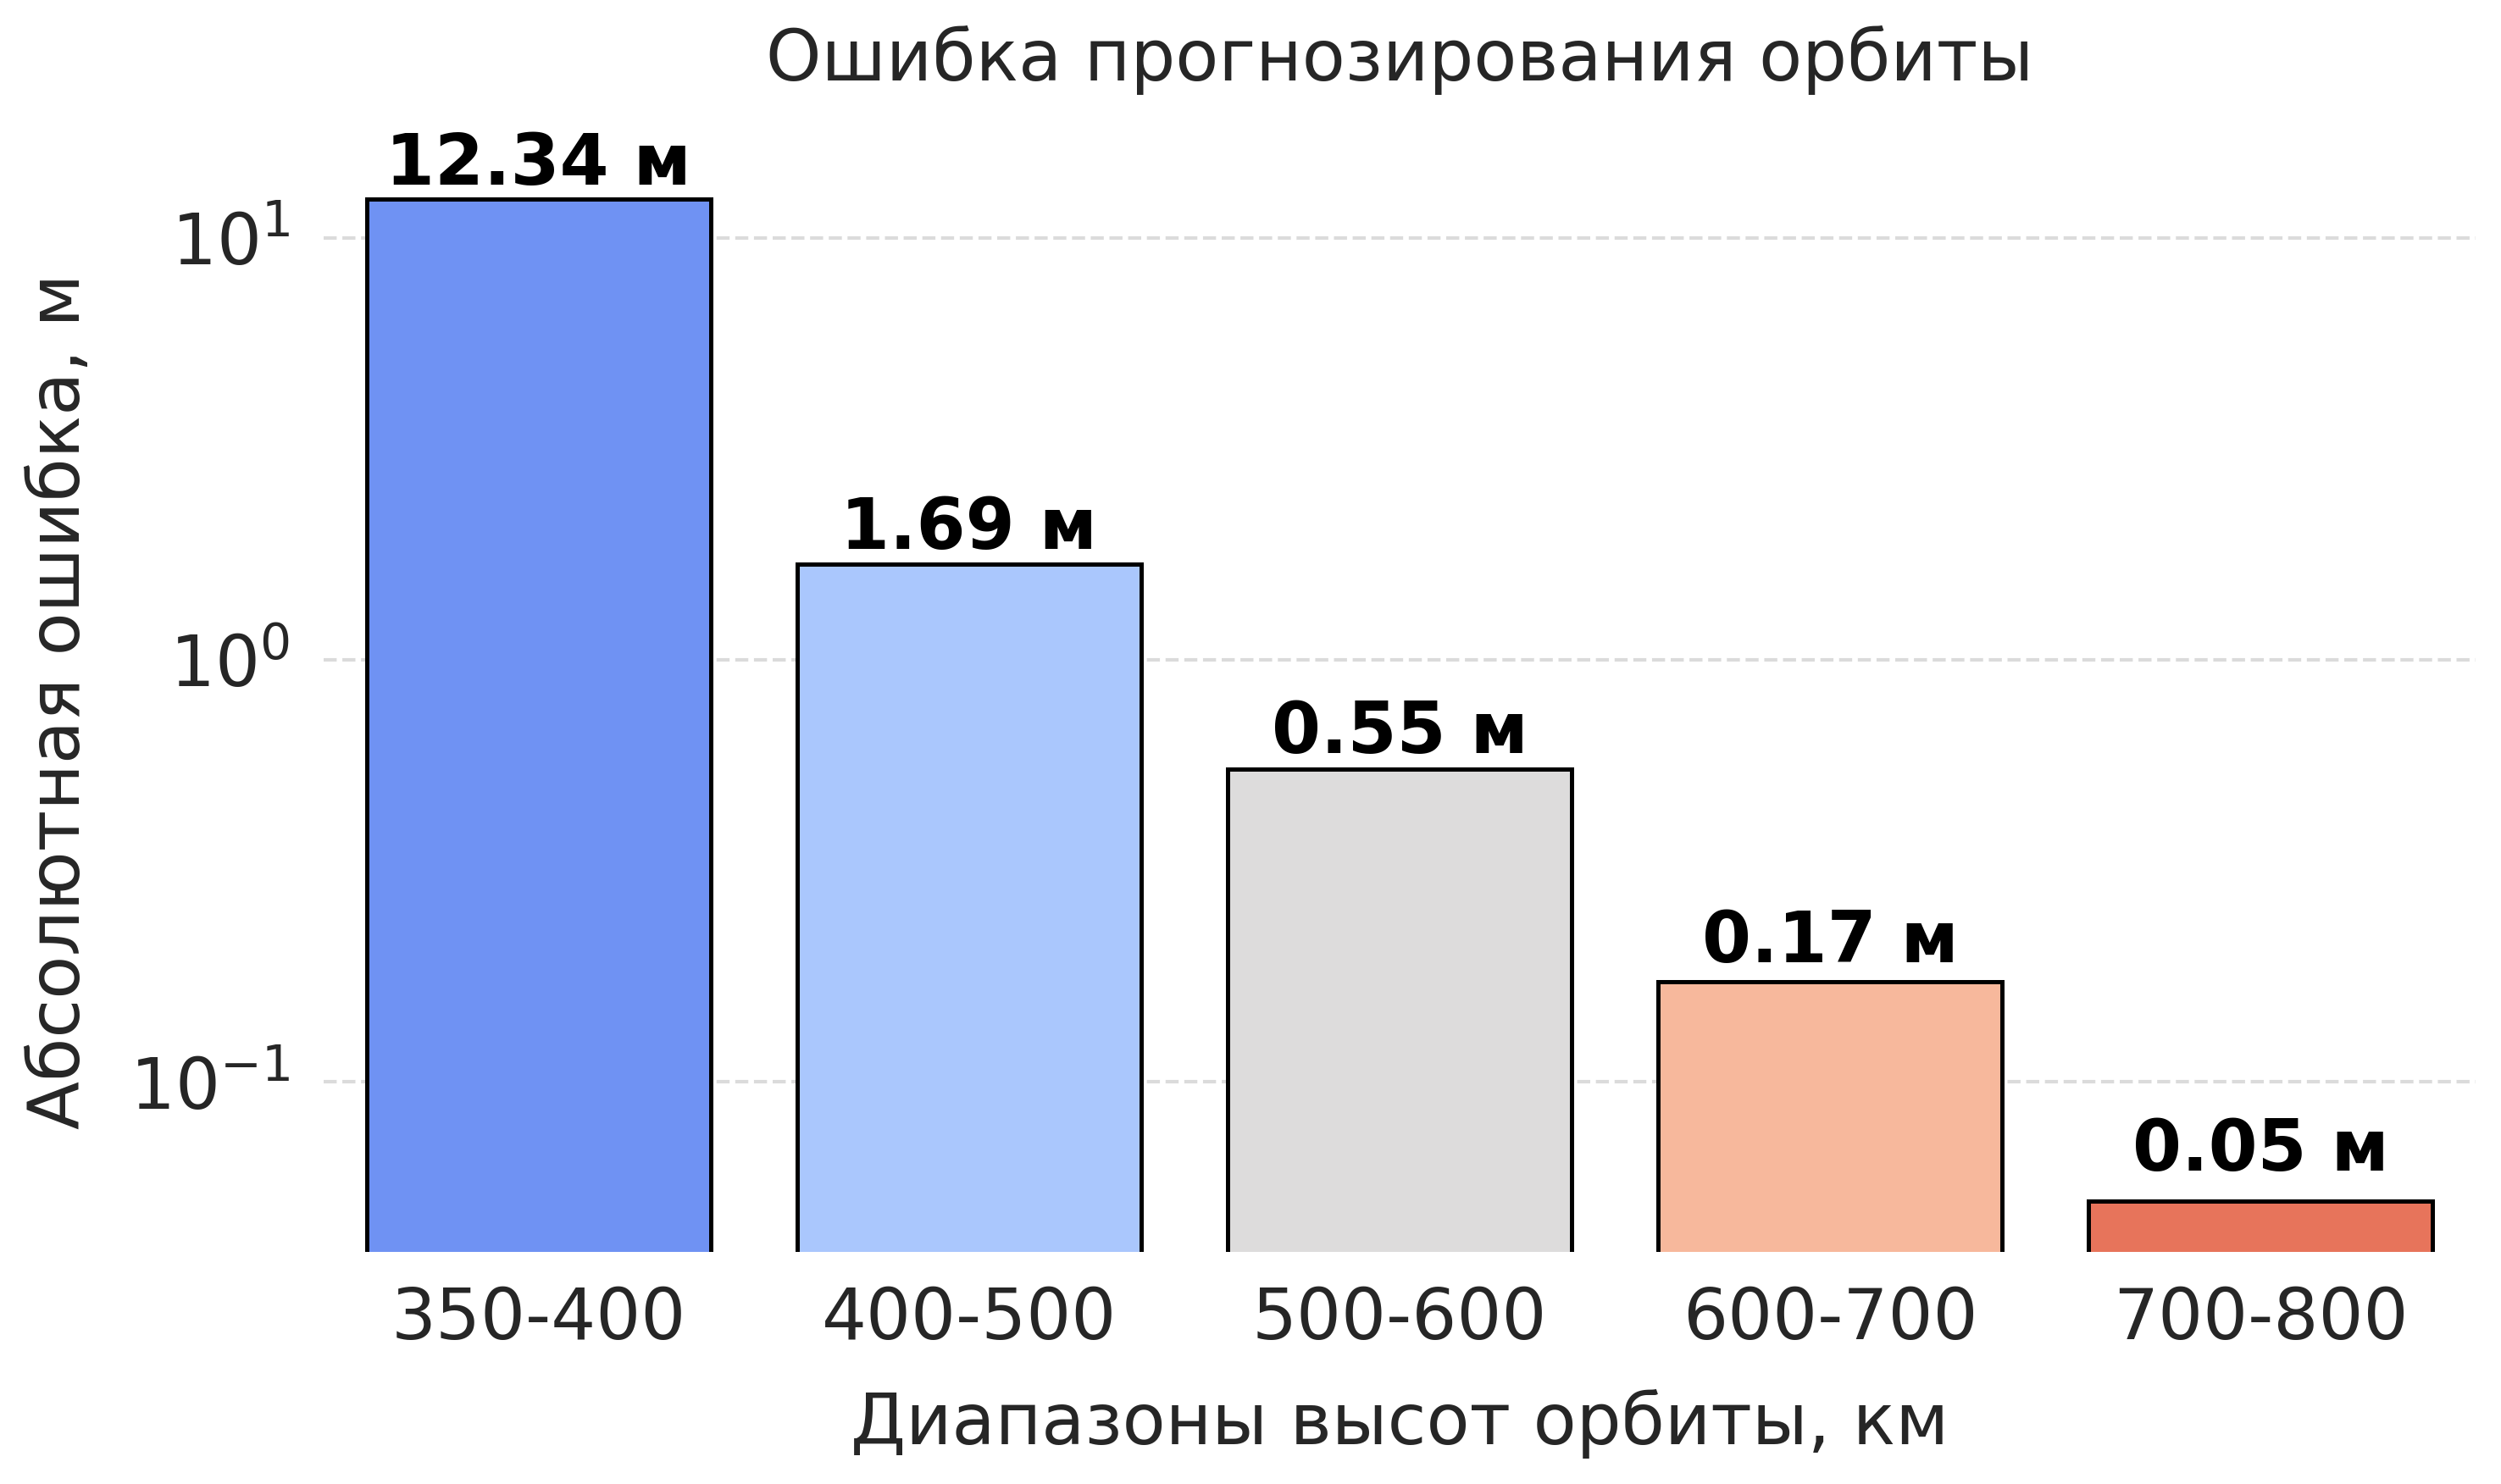
\includegraphics[width=\linewidth]{../images/solution/atmo/propagation/2537.png}
        \caption{Конфигурация (2, 5, 3, 7),
        количество ячеек (65, 25, 50, 20)}
        \label{fig:atmo:2537_propag}
    \end{subfigure}
    
    \vspace{0.5cm} % Вертикальный отступ между строками
    
    % Третья строка
    \begin{subfigure}[b]{0.48\textwidth}
        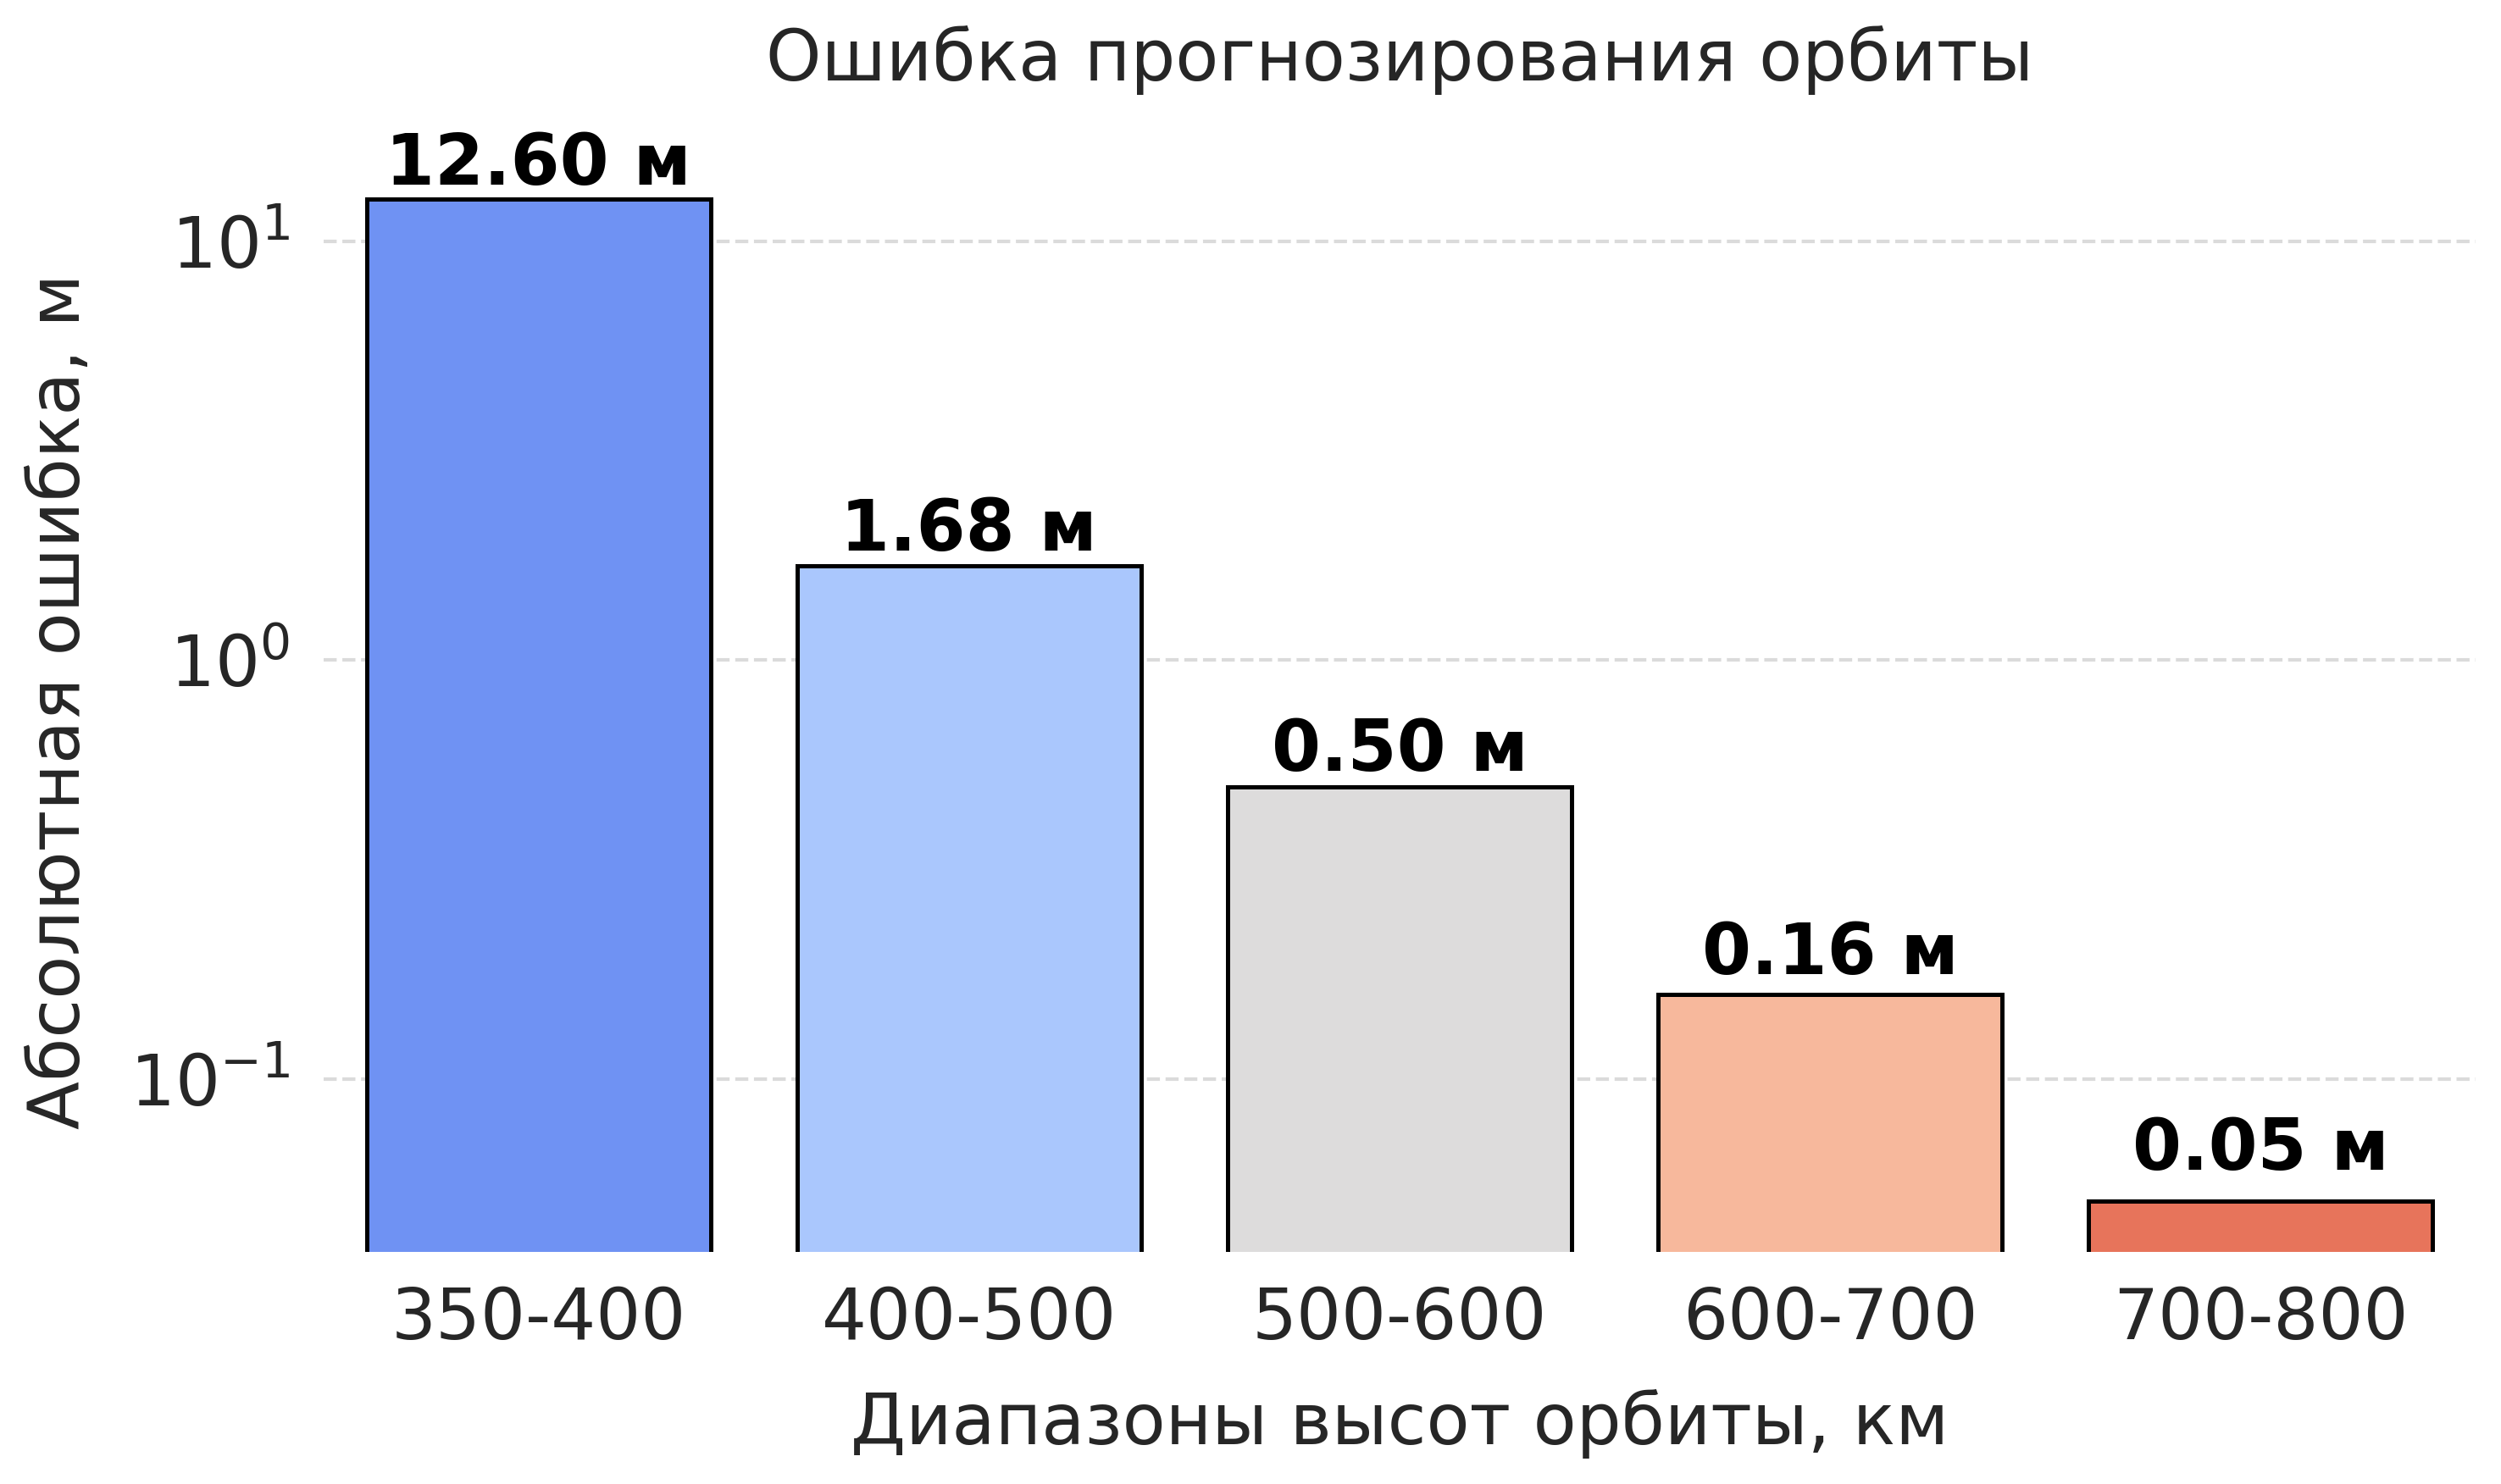
\includegraphics[width=\linewidth]{../images/solution/atmo/propagation/2573.png}
        \caption{Конфигурация (2, 5, 7, 3),
        количество ячеек (65, 25, 20, 50)}
        \label{fig:atmo:2573_propag}
    \end{subfigure}
    \hfill
    \begin{subfigure}[b]{0.48\textwidth}
        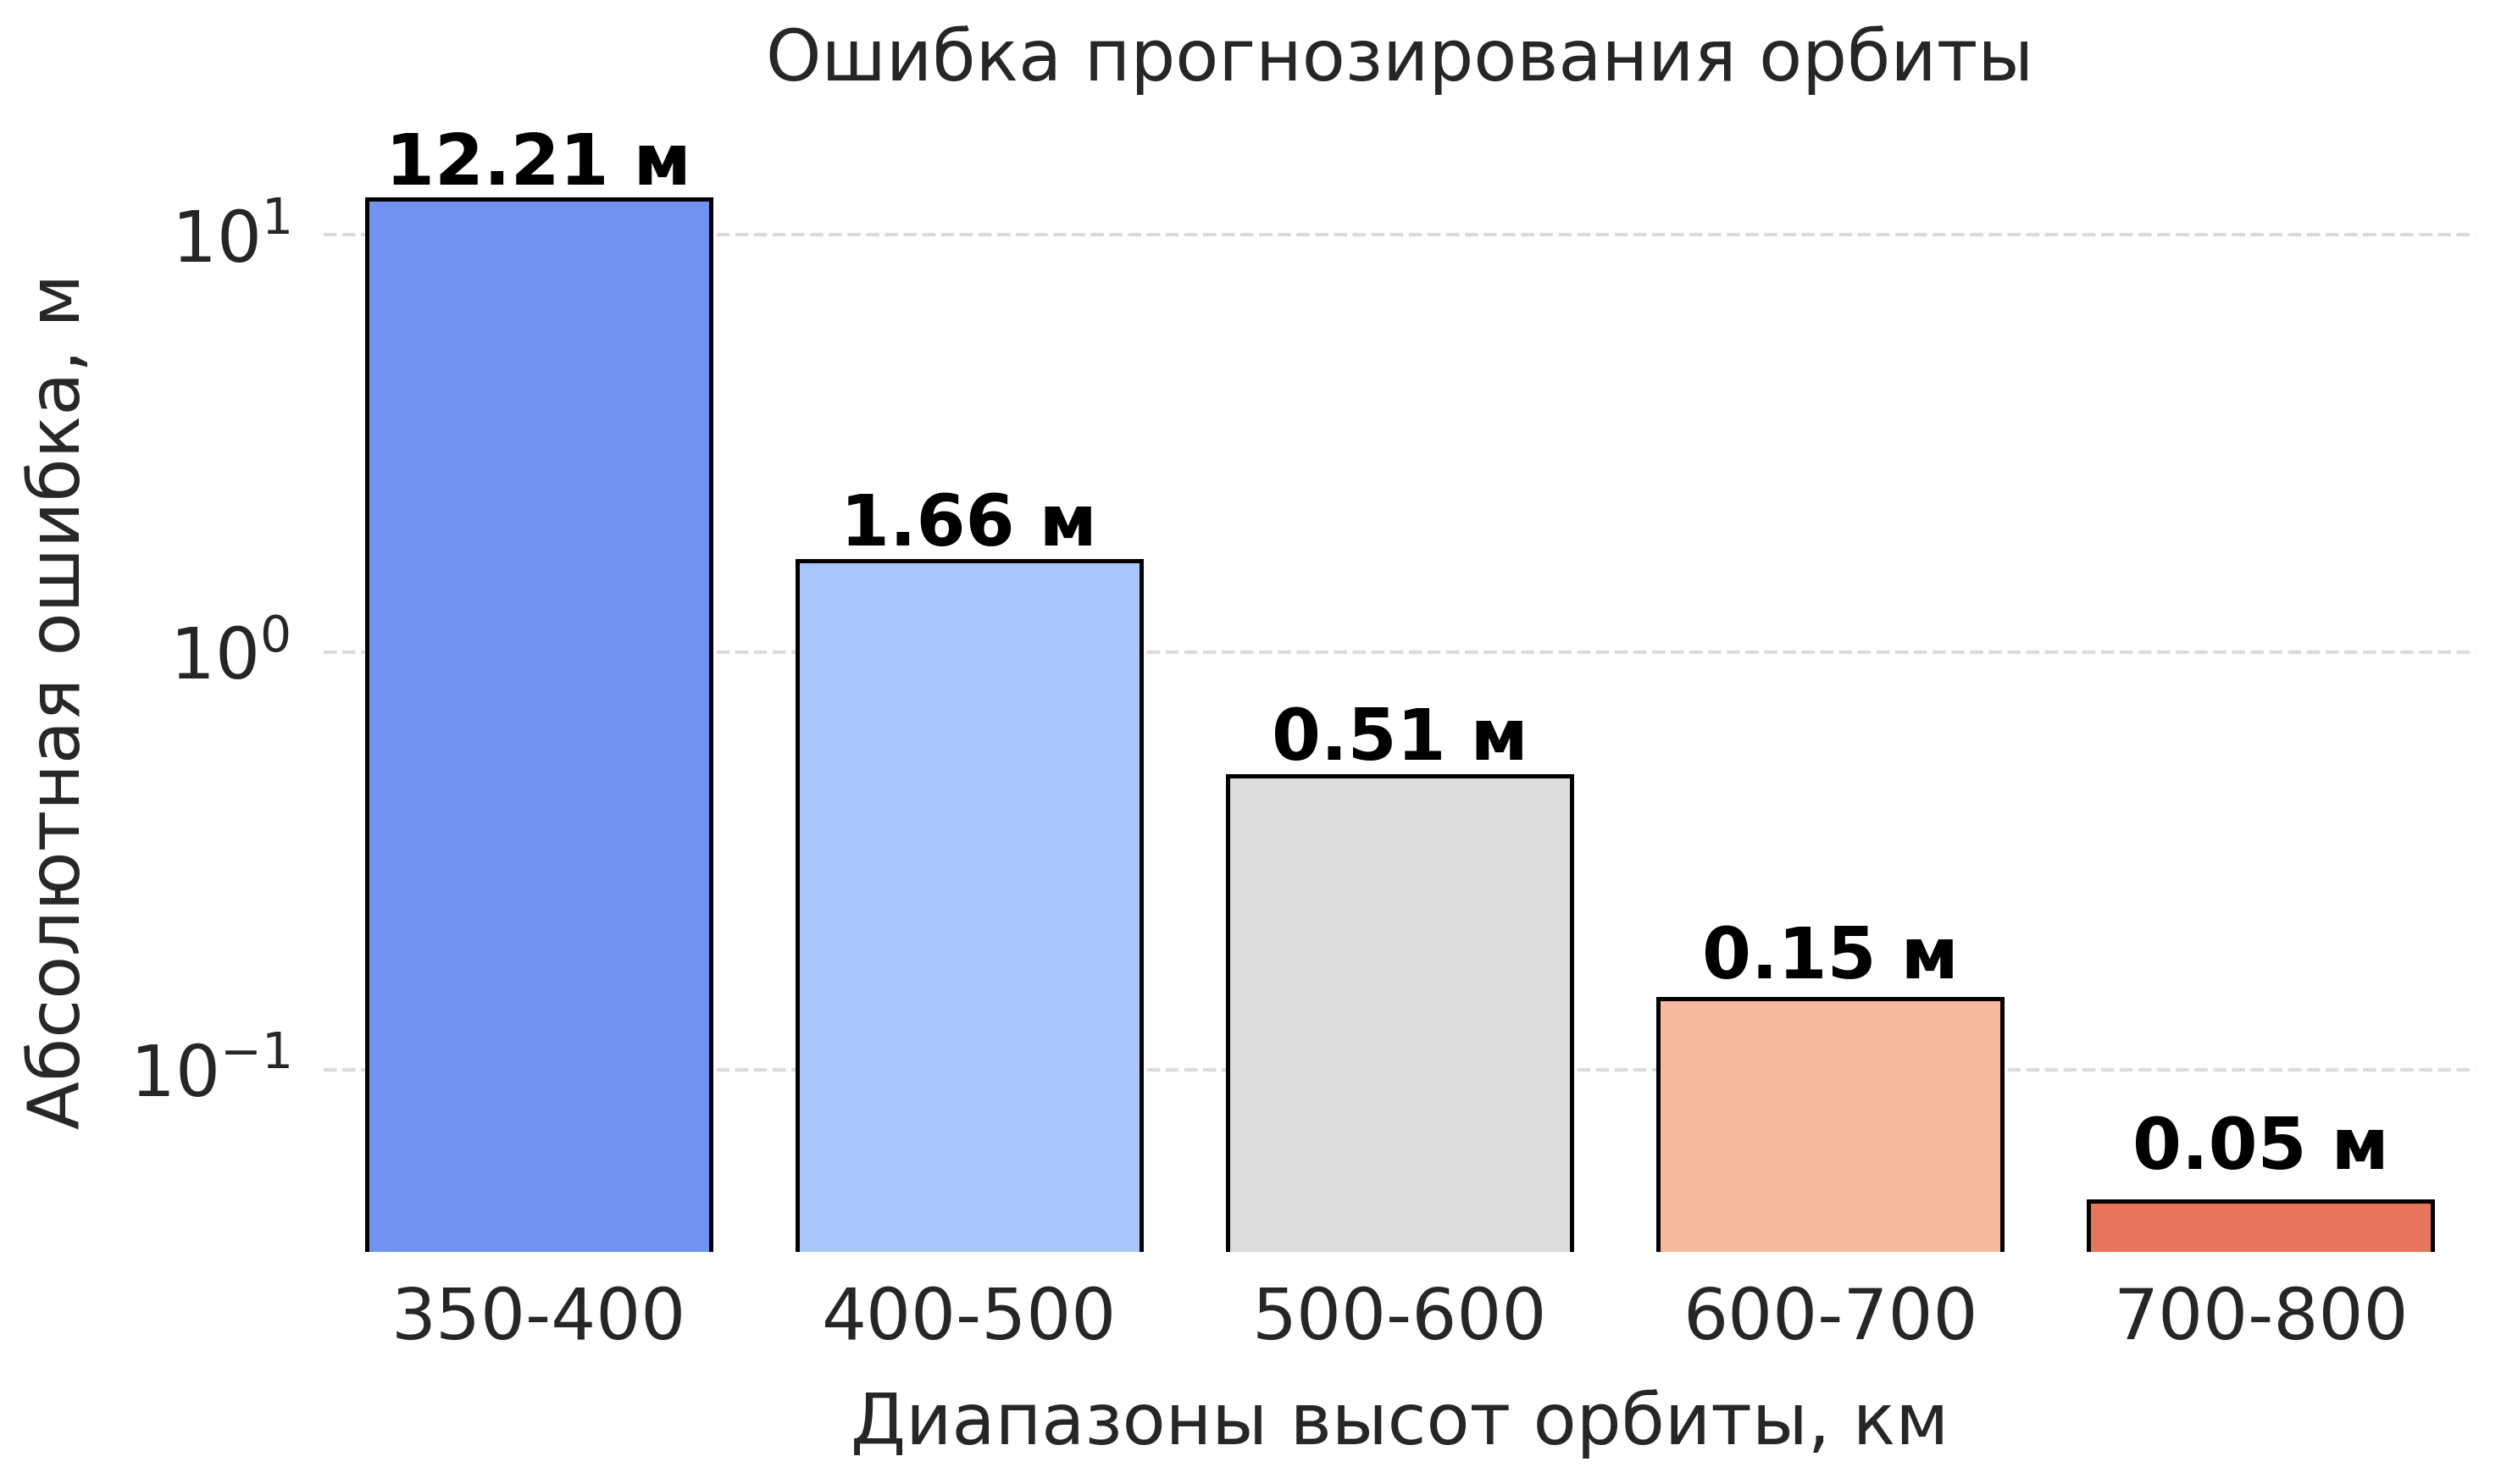
\includegraphics[width=\linewidth]{../images/solution/atmo/propagation/2735.png}
        \caption{Конфигурация (2, 7, 3, 5),
        количество ячеек (65, 15, 45, 40)}
        \label{fig:atmo:2735_propag}
    \end{subfigure}
    \caption{Зависимость ошибки прогнозирования от высоты}
    \label{fig:all_images}
\end{figure}

На заключительной стадии оценивалась возможность совместного применения интерполянтов
плотности и атмосферы. Рассмотрены орбиты с предыдущего этапа тестирования. 
Интерполянт гравитации строился по конфигурации (13, 14, 15) с числом ячеек (10, 35, 70)
на основе модели EGM2008 с 64 гармониками.
Прогноз был выполнен на 1 день. 

Сводные результаты приведены в таблице \ref{tab:atmo_propag_acc}. Из результатов следует, что интерполировать атмосферу
при прямом вычислении силы гравитационного притяжения нецелесообразно, так как ускорение
получается незначительным, в то время как появляется существенная ошибка. Интерполяция
как гравитации, так и атмосферы позволяет рассчитывать траекторию с шестикратным ускорением и
ошибкой не более 12 метров (для низких орбит).

Дальнейший анализ интерполяции атмосферы может быть связан с совершенствованием методики
поиска рациональных конфигураций и разбиений. В частности, рекомендуется
построить интерполянты с б\`{о}льшим количеством ячеек по разным координатам. Для ускорения
перебора следует использовать эмпирические зависимости, полученные из представленных в работе
результатов.

\begin{table}[h!]
    \caption{Сводная таблица скорости прогноза}
    \centering
    \renewcommand{\arraystretch}{1.5}
    \begin{tabular}{|ll|ll|}
    \hline
    \multicolumn{2}{|l|}{\multirow{2}{*}{Относительная скорость прогноза}} & \multicolumn{2}{c|}{Гравитация}                         \\ \cline{3-4} 
    \multicolumn{2}{|l|}{}                                                 & \multicolumn{1}{c|}{Без интерполяции} & С интерполяцией \\ \hline
    \multicolumn{1}{|l|}{\multirow{2}{*}{Атмосфера}}   & Без интерполяции  & \multicolumn{1}{l|}{1}                & 2.8             \\ \cline{2-4} 
    \multicolumn{1}{|l|}{}                             & С интерполяцией   & \multicolumn{1}{l|}{1.2}              & 5.7             \\ \hline
    \end{tabular}
    \label{tab:atmo_propag_acc}
\end{table}
\clearpage